% \section{Detailed results Oct-Dec 2023}\label{app:results}

% \includepdf[pages=-, scale=0.8]{content/December 22 recap.pdf}

% \includepdf[pages=1,scale=.8,pagecommand={\section{Detailed results Oct-Dec 2023}\label{app:results}},linktodoc=true]{content/December 22 recap.pdf}
% \includepdf[pages=2-,scale=.8,pagecommand={},linktodoc=true]{content/December 22 recap.pdf}

% \begin{figure*}[tb]
%     \centering
%     \includegraphics[width=1\linewidth]{app_content/misc/Poster_architecture_diagram.pdf}
%     \caption{Architecture diagram for DRED.}
%     \label{fig:DRED-diagram}
% \end{figure*}

\section{Theoretical results}\label{app:proofs}

\begin{lemma}
    Given a set of training levels $L$ and an agent model $\pi = f \circ b$, where $b(H^o_t) = h_t \in \sB$ is an intermediate representation function and $f : \sB \rightarrow \Delta^\sA$ maps to the agent's action distribution, we have
    \begin{align}
        \mut{L}{\pi} \leq \entropy(\ri) + \sum_{i\in L} \int_{\sB} p(h, i) \log p(i|h)dh,
    \end{align}
    where the right-hand side is equivalent to $\mut{L}{b}$.

    proof:
    
    Since the information chain of our model follows $H_t^o \rightarrow b \rightarrow f$, we have $\mut{L}{f \circ b} \leq \mut{L}{b}$, from the data processing inequality. $\mut{L}{b}$ can then be manipulated as follows
    \begin{align}\label{eq:proof_mi_kld}
    % \begin{split}
        \mut{L}{b} &= \sum_{i \in L} \int_{\sB} p(h,i) \log \frac{p(h,i)}{p(h)p(i)}dh \\
        &= - \sum_{i \in L} \int_{\sB} p(h,i) \log p(i) dh + \sum_{i \in L} \int_{\sB} p(h, i) \log p(i|h) dh \\
        &= \entropy(\ri) + \sum_{i\in L} \int_{\sB} p(h, i) \log p(i|h)dh.
    % \end{split}
    \end{align}

\end{lemma}


% To main text:
    % &\approx \mathcal{H}(p(\ri)) + \frac{1}{|B|} \sum^{|B|}_{n} \log p(i^{(n)}|\vh^{(n)}) \label{eq:proof_empirical_approx}

    % where in \cref{eq:proof_empirical_approx} we approximate $p(\vh,i)$ as the empirical distribution

    % \begin{equation} \label{eq:empirical_approx}
    %     \tilde{p}(\vh,i) = 
    %     \begin{cases}
    %         \frac{1}{|B|} &\text{ if } (H_t^o, i) \in B, \text{ with } \vh = b(H_t^o) \\
    %         0 &\text{ otherwise.}
    %     \end{cases}
    % \end{equation}
    
\section{Procgen additional experimental results}\label{app:results_procgen}

\subsection{Measuring the relationship between $\mut{L}{b}$ and the $\text{GenGap}$ across sampling methods and procgen games}\label{app:mi_gengap}

\begin{table}[!htb]
\caption{$\mut{L}{b}$ measured under different adaptive sampling strategies. We report aggregated $\mut{L}{b}$ across 5 training runs, each initialised with a different seed. To compute $\mut{L}{b}$ for each run and environment, we first fit a linear classifier $p_\vtheta$ to predict level identities from the agent's penultimate layer outputs, using rollouts from levels sampled uniformly from $L$. We then estimate $\mut{L}{b}$ using \Cref{eq:mi_empirical_approx}, using a different set of rollouts also sampled uniformly from $L$. In the last row we compute the mean $\mut{L}{b}$  across environments for each run, and we report the mean and standard deviation of that quantity across all runs. Bolded methods are not significantly different from the method with lowest mean ($p<0.05$), unless all are, in which case none are bolded.}
\label{tb:procgen_mi}
\vskip 0.15in
\begin{center}
\begin{small}
\begin{sc}
\begin{tabular}{lrrrrr}
\toprule
               Environment &                  $S=S^V$ &        $P_S=\mathcal{U}$ &      $S=S^{\mathrm{MI}}$ & $S=S^V, P_{S^\prime}=\mathcal{U}$ & $S=S^V, S^\prime=S^{\mathrm{MI}}$ \\
\midrule
                   Bigfish & \textbf{1.74 $\pm$ 0.36} &          4.33 $\pm$ 0.48 & \textbf{1.45 $\pm$ 0.36} &                   2.43 $\pm$ 0.53 &          \textbf{1.77 $\pm$ 0.70} \\
                     Heist &          4.67 $\pm$ 0.31 & \textbf{3.68 $\pm$ 0.36} & \textbf{4.08 $\pm$ 0.50} &                   4.54 $\pm$ 0.37 &                   4.76 $\pm$ 0.19 \\
                   Climber &          4.03 $\pm$ 0.23 &          4.40 $\pm$ 0.18 & \textbf{2.44 $\pm$ 0.44} &                   4.48 $\pm$ 0.15 &                   4.09 $\pm$ 0.17 \\
                 Caveflyer &          3.01 $\pm$ 0.17 &          3.94 $\pm$ 0.21 & \textbf{1.72 $\pm$ 0.20} &                   3.38 $\pm$ 0.14 &                   3.00 $\pm$ 0.18 \\
                    Jumper &          4.49 $\pm$ 0.13 & \textbf{3.87 $\pm$ 0.40} & \textbf{3.38 $\pm$ 0.38} &                   4.37 $\pm$ 0.19 &                   4.39 $\pm$ 0.07 \\
                  Fruitbot & \textbf{0.15 $\pm$ 0.09} &          2.76 $\pm$ 0.11 &          0.40 $\pm$ 0.17 &                   0.24 $\pm$ 0.09 &          \textbf{0.09 $\pm$ 0.07} \\
                   Plunder &          1.46 $\pm$ 0.22 &          2.95 $\pm$ 0.74 & \textbf{1.09 $\pm$ 0.20} &                   1.80 $\pm$ 0.41 &                   1.76 $\pm$ 0.22 \\
                   Coinrun & \textbf{1.38 $\pm$ 0.07} &          2.29 $\pm$ 0.19 & \textbf{1.30 $\pm$ 0.14} &                   1.59 $\pm$ 0.05 &          \textbf{1.36 $\pm$ 0.15} \\
                     Ninja &          2.36 $\pm$ 0.30 &          2.62 $\pm$ 0.24 & \textbf{1.42 $\pm$ 0.44} &                   3.00 $\pm$ 0.17 &                   2.45 $\pm$ 0.19 \\
                    Leaper &          1.72 $\pm$ 0.08 &          1.06 $\pm$ 0.08 & \textbf{0.79 $\pm$ 0.13} &                   1.79 $\pm$ 0.22 &                   1.65 $\pm$ 0.18 \\
                      Maze &          4.76 $\pm$ 0.09 & \textbf{4.27 $\pm$ 0.22} &          4.79 $\pm$ 0.15 &                   4.73 $\pm$ 0.09 &                   4.72 $\pm$ 0.04 \\
                     Miner & \textbf{4.36 $\pm$ 0.13} &          4.81 $\pm$ 0.02 & \textbf{4.42 $\pm$ 0.27} &          \textbf{4.53 $\pm$ 0.22} &          \textbf{4.29 $\pm$ 0.17} \\
                 Dodgeball &          3.88 $\pm$ 0.37 &          2.51 $\pm$ 0.32 & \textbf{0.89 $\pm$ 0.34} &                   4.05 $\pm$ 0.19 &                   3.54 $\pm$ 0.41 \\
                 Starpilot & \textbf{1.10 $\pm$ 0.06} &          2.07 $\pm$ 0.14 &          1.38 $\pm$ 0.11 &                   1.44 $\pm$ 0.13 &          \textbf{1.20 $\pm$ 0.08} \\
                    Chaser & \textbf{1.37 $\pm$ 0.12} &          3.18 $\pm$ 0.26 & \textbf{1.36 $\pm$ 0.14} &                   1.98 $\pm$ 0.34 &          \textbf{1.43 $\pm$ 0.25} \\
                 Bossfight & \textbf{1.33 $\pm$ 0.12} &          4.19 $\pm$ 0.35 & \textbf{1.17 $\pm$ 0.12} &          \textbf{1.15 $\pm$ 0.17} &          \textbf{1.16 $\pm$ 0.33} \\
\midrule
Average Mutual Information &          2.61 $\pm$ 0.05 &          3.31 $\pm$ 0.03 & \textbf{2.00 $\pm$ 0.07} &                   2.84 $\pm$ 0.08 &                   2.60 $\pm$ 0.02 \\
\bottomrule
\end{tabular}
\end{sc}
\end{small}
\end{center}
\vskip -0.1in
\end{table}

\begin{table}[!htb]
\caption{Level classifier accuracies measured under different adaptive sampling strategies. We report aggregated accuracies across 5 training runs, each initialised with a different seed. To compute this quantity for each run and environment, we first fit a linear classifier $p_\vtheta$ to predict level identities from the agent's penultimate layer outputs, using rollouts from levels sampled uniformly from $L$. We then measure the classifier accuracy, using a different set of rollouts also sampled uniformly from $L$. In the last row we compute the mean accuracy across environments for each run, and we report the mean and standard deviation of that quantity across all runs. Bolded methods are not significantly different from the method with lowest mean ($p<0.05$), unless all are, in which case none are bolded.}
\label{tb:procgen_accuracy}
\vskip 0.15in
\begin{center}
\begin{small}
\begin{sc}
\begin{tabular}{lrrrrr}
\toprule
                Environment &                  $S=S^V$ &       $P_S=\mathcal{U}$ &      $S=S^{\mathrm{MI}}$ & $S=S^V, P_{S^\prime}=\mathcal{U}$ & $S=S^V, S^\prime=S^{\mathrm{MI}}$ \\
\midrule
                    Bigfish & \textbf{17.2 $\pm$ 10.1} &          66.5 $\pm$ 5.5 &  \textbf{12.8 $\pm$ 4.5} &          \textbf{24.7 $\pm$ 10.3} &           \textbf{14.3 $\pm$ 9.9} \\
                      Heist &           83.1 $\pm$ 9.5 &          77.8 $\pm$ 3.8 & \textbf{38.1 $\pm$ 20.7} &                    77.5 $\pm$ 5.6 &                    72.5 $\pm$ 9.1 \\
                    Climber &          53.4 $\pm$ 15.0 &          82.9 $\pm$ 3.3 & \textbf{17.4 $\pm$ 10.5} &                    73.2 $\pm$ 3.6 &                    64.0 $\pm$ 5.6 \\
                  Caveflyer &           34.9 $\pm$ 5.4 &          62.5 $\pm$ 3.9 &  \textbf{21.4 $\pm$ 1.5} &                    48.5 $\pm$ 6.0 &          \textbf{33.1 $\pm$ 11.5} \\
                     Jumper &          62.0 $\pm$ 10.4 &          64.4 $\pm$ 6.3 & \textbf{28.0 $\pm$ 17.8} &                    64.1 $\pm$ 5.6 &                   59.4 $\pm$ 10.0 \\
                   Fruitbot &   \textbf{2.7 $\pm$ 4.1} &          18.0 $\pm$ 1.3 &   \textbf{5.3 $\pm$ 6.9} &            \textbf{2.6 $\pm$ 2.0} &            \textbf{2.3 $\pm$ 2.8} \\
                    Plunder &  \textbf{13.5 $\pm$ 9.8} &          25.3 $\pm$ 8.8 &   \textbf{2.6 $\pm$ 3.4} &                    16.1 $\pm$ 6.8 &           \textbf{15.5 $\pm$ 9.9} \\
                    Coinrun &  \textbf{14.1 $\pm$ 0.8} &          22.3 $\pm$ 1.9 &  \textbf{10.5 $\pm$ 4.7} &           \textbf{11.6 $\pm$ 4.0} &           \textbf{13.4 $\pm$ 4.2} \\
                      Ninja &           22.8 $\pm$ 7.5 &          33.9 $\pm$ 2.4 &   \textbf{5.6 $\pm$ 7.2} &                    27.8 $\pm$ 2.9 &                    18.4 $\pm$ 4.9 \\
                     Leaper &           10.2 $\pm$ 5.6 &          11.6 $\pm$ 2.1 &            8.5 $\pm$ 4.0 &                    13.0 $\pm$ 1.0 &                    12.9 $\pm$ 3.2 \\
                       Maze &           69.7 $\pm$ 2.6 & \textbf{65.5 $\pm$ 1.3} & \textbf{69.2 $\pm$ 10.2} &           \textbf{63.9 $\pm$ 3.8} &           \textbf{67.7 $\pm$ 7.8} \\
                      Miner &           85.5 $\pm$ 1.1 &          92.0 $\pm$ 0.7 &  \textbf{67.7 $\pm$ 8.2} &                    80.4 $\pm$ 4.3 &           \textbf{78.1 $\pm$ 4.5} \\
                  Dodgeball &           63.1 $\pm$ 0.8 &          45.4 $\pm$ 7.3 &   \textbf{5.7 $\pm$ 5.8} &                    68.5 $\pm$ 7.5 &                    53.5 $\pm$ 7.4 \\
                  Starpilot &            8.1 $\pm$ 3.1 &          14.7 $\pm$ 3.3 &   \textbf{3.2 $\pm$ 2.4} &                     9.0 $\pm$ 2.7 &                     6.8 $\pm$ 1.1 \\
                     Chaser &  \textbf{13.0 $\pm$ 3.3} &          40.4 $\pm$ 4.7 &   \textbf{7.8 $\pm$ 4.0} &                   27.7 $\pm$ 12.3 &           \textbf{16.2 $\pm$ 6.1} \\
                  Bossfight &   \textbf{6.9 $\pm$ 6.1} &         60.2 $\pm$ 14.3 &   \textbf{3.1 $\pm$ 4.1} &           \textbf{10.4 $\pm$ 6.2} &           \textbf{10.5 $\pm$ 8.5} \\
\midrule
Average Classifier Accuracy &           35.0 $\pm$ 1.7 &          49.0 $\pm$ 0.9 &  \textbf{19.2 $\pm$ 2.2} &                    38.7 $\pm$ 1.3 &                    33.7 $\pm$ 1.6 \\
\bottomrule
\end{tabular}
\end{sc}
\end{small}
\end{center}
\vskip -0.1in
\end{table}

To better understand the interaction between the mutual information, the value loss and the generalisation gap, we plot our estimate for $\mut{L}{b}$ at the end of training against the $\text{GenGap}$ and the $\ell_1$-value loss for all methods tested and across Procgen games in \Cref{fig:correlation_analysis}. We find a positive correlation (correlation coefficient $\rho=0.60$) and rank correlation (Kendall rank correlation coefficient $\xi=0.50, p<1e-50$) between $\mut{L}{b}$ and the $\text{GenGap}$. We find similar correlation ($\rho=0.50$) and rank correlation ($\xi=0.49, p<1e-47$) between $\mut{L}{b}$ and the normalised $\text{GenGap}$. We also observe a weaker but statistically significant negative correlation ($\rho=-0.18$) and negative rank correlation ($\xi=-0.11, p<0.001$) between $\mut{L}{b}$ and the $\ell_1$-value loss. 

We report the $\mut{L}{b}$ averaged across seeds for all games and methods tested in \Cref{tb:procgen_mi}. In order to obtain a more intuitive quantification of $\mut{L}{b}$, we also report the classification accuracy of the linear classifier $p_\vtheta$ in \Cref{tb:procgen_accuracy}, as these two quantities are proportional to one-another. Out of 200 training levels, the classifier correctly predicts the current level $49\%$ of the times under uniform sampling, $35\%$ under $(S=S^V)$ and $19\%$ under $S^{\text{MI}}$. While adaptive sampling strategies are able to significantly reduce $\mut{L}{b}$, the mean classifier accuracy is still $70$ times random guessing for $(S=S^V)$ and $38$ times random guessing for $(S=S^{\text{MI}})$.

\begin{figure}[!htb]
\centering
    \begin{subfigure}{0.49\linewidth}
            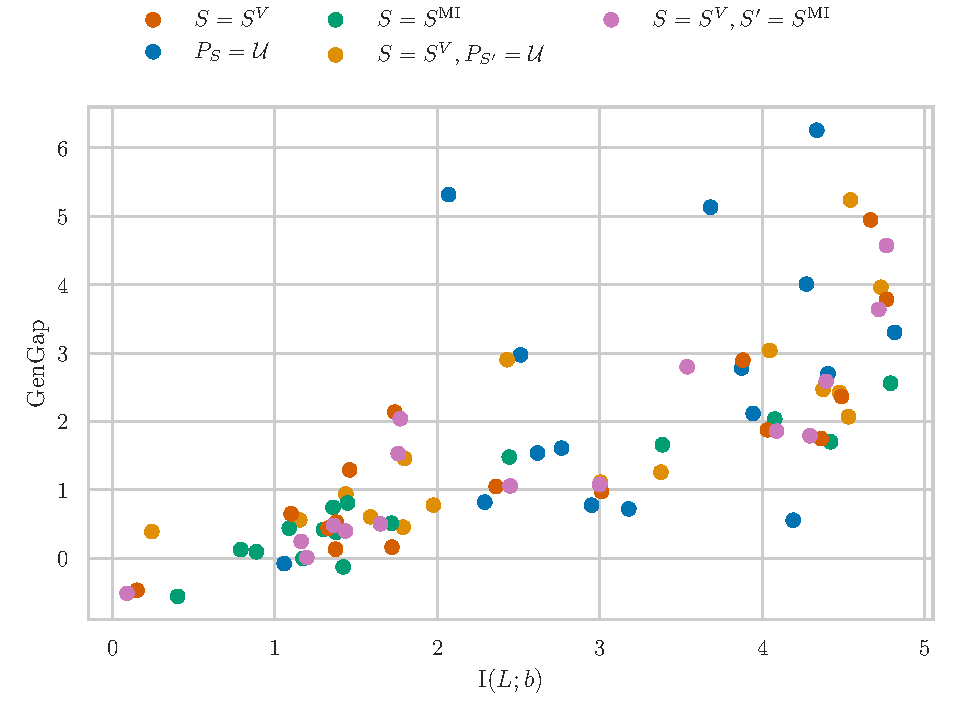
\includegraphics[width=1\linewidth]{app_content/procgen/MI_gengap_scatter.pdf}
    \end{subfigure}%
    \begin{subfigure}{0.49\linewidth}
            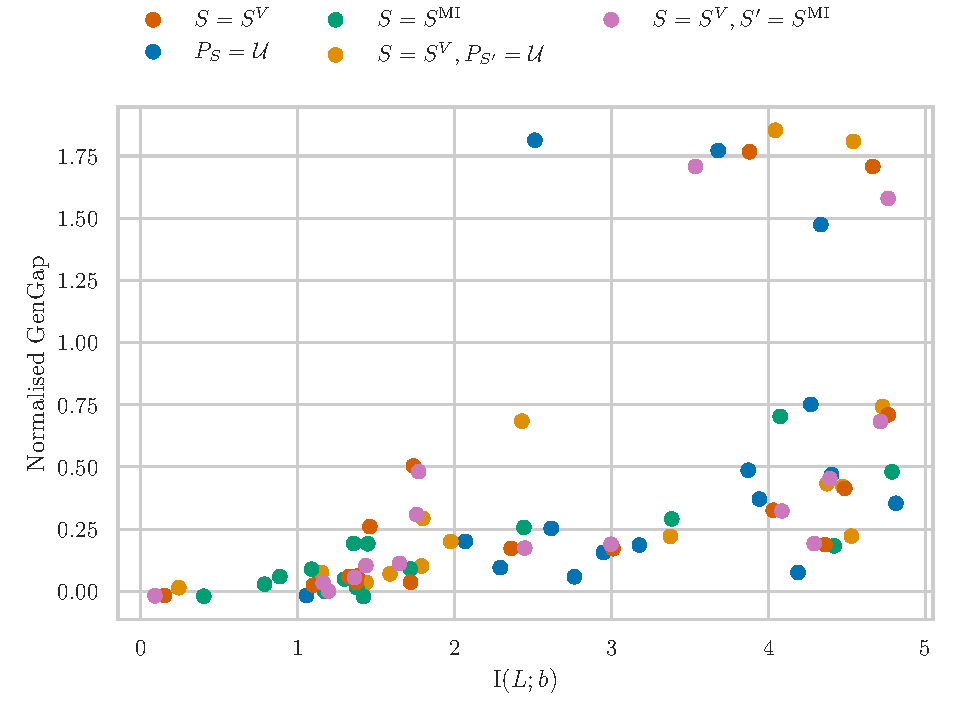
\includegraphics[width=1\linewidth]{app_content/procgen/MI_normgengap_scatter.pdf}
    \end{subfigure}\\%
    \begin{subfigure}{0.49\linewidth}
            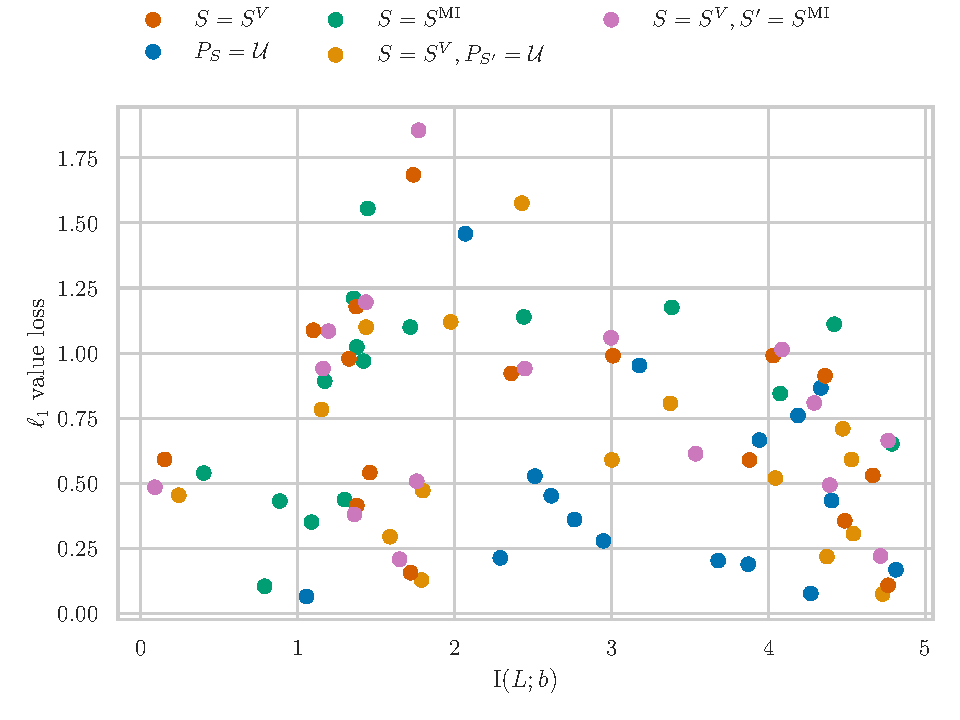
\includegraphics[width=1\linewidth]{app_content/procgen/MI_vl_scatter.pdf}
    \end{subfigure}%
    \caption{Scatter plot displaying how $\mut{L}{b}$ compares to the $\text{GenGap}$ (top left), to the normalised $\text{GenGap}$ (top right), and to the $\ell_1$ average value loss (bottom) across all methods and Procgen games, at the end of training. Each plotted point represents the average of 5 seeds in a particular game.}\label{fig:correlation_analysis}
\end{figure}

% To further reduce $\mut{L}{b}$, adaptive sampling could be combined with other data regularisation techniques, such as performing level set augmentation as it was proposed in this work. Other data augmentation techniques also synergise well with adaptive sampling strategies: \cite{PLR} report a significant improvement in test scores when combining PLR with UCB-DrAC \cite{raileanu2021UCB-DrAC}, an observation augmentation method. 

\subsection{A qualitative analysis of when adaptive sampling strategies may or may not be effective in reducing the $\text{GenGap}$}\label{app:procgen_level_analysis}

\begin{figure}[!htb]
\centering
    \begin{subfigure}{0.49\linewidth}
            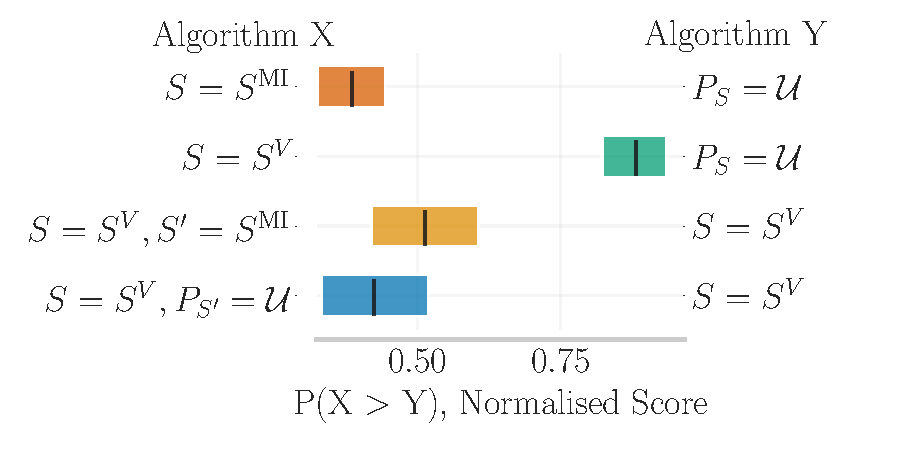
\includegraphics[width=1\linewidth]{app_content/procgen/procgen_prob_of_improvement.pdf}
    \end{subfigure}%
    \begin{subfigure}{0.49\linewidth}
            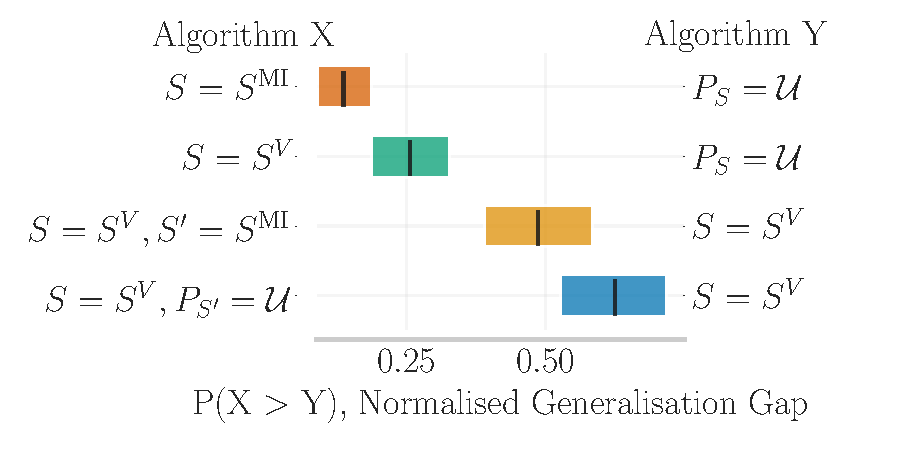
\includegraphics[width=1\linewidth]{app_content/procgen/procgen_prob_of_improvement_gap.pdf}
    \end{subfigure}%
    \caption{Probability of algorithm $X$ incurring a higher normalised test score (left) and $\text{GenGap}$ (right) than algorithm $Y$. Colored boxes indicate the 95\% confidence interval.}\label{fig:p_improvement_procgen}
\end{figure}

%TODO: refer to table when added
We report in \Cref{fig:p_improvement_procgen} that, when compared to uniform sampling across procgen games, adaptive sampling strategies are significantly more likely to reduce the $\text{GenGap}$. Strategies employing ($S=S^V$) as their primary scoring function are also more likely to improve their test set scores. However, we measure significant variability across procgen games  for $\mut{L}{b}$ in \Cref{tb:procgen_mi} (and by extension for the $\text{GenGap}$) for the different strategies tested. To better understand why, we compare the measured accuracy with a qualitative analysis of the observations and levels encountered in the ``Maze'' and ``Bigfish'' games (see \Cref{fig:procgen_levels} for renderings of different levels from each game). In Maze, the classifier accuracy remains over $60\%$ ($120\times$ random) for all methods tested and the reduction in $\text{GenGap}$ is insignificant. On the other hand, in Bigfish all adaptive sampling strategies tested lead to a significant reduction in classifier accuracy when compared to uniform sampling, dropping from $65\%$ to between $12\%$ and $25\%$ (depending on the strategy), and correspond to a significant drop in the $\text{GenGap}$ and improvement in test scores. 

\begin{figure}[!htb]
\centering
    \begin{subfigure}{0.3\linewidth}
            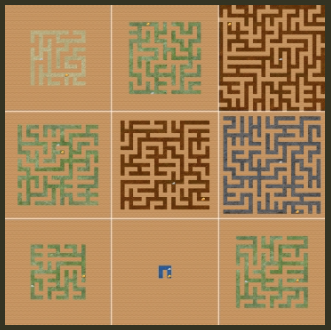
\includegraphics[width=1\linewidth]{app_content/procgen/maze.png}
    \end{subfigure}%
    \begin{subfigure}{0.3\linewidth}
        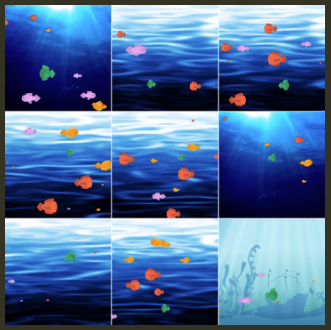
\includegraphics[width=1\linewidth]{app_content/procgen/bigfish.png}
    \end{subfigure}%
    \caption{Agent observations sampled from 9 levels from the Maze (left) and Bigfish (right) games of the Procgen benchmark.}\label{fig:procgen_levels}
\end{figure}

In Maze, the observation space lets the agent observe the full layout at every timestep. The maze layout is unique to each level and should be easily identifiable by the agent's ResNet architecture. Intuitively, we can hypothesise that adaptive sampling strategies will not be effective if all the levels are easily identifiable by the model, which appears to be the case in Maze. In these cases, other data regularisation techniques, such as augmenting the observations, could be more effective, and in fact \cite{PLR} report that Maze is one of the games where combining PLR with UCB-DrAC \cite{raileanu2021UCB-DrAC}, a data augmentation method, leads to a significant improvement in test scores.

On the other hand, we observe that many of the Bigfish levels yield similar observations. Indeed, both the features relevant to the task (the fish) and irrelevant (the background) are similar in many of the training levels. Furthermore, there's significant variation in the observations encountered during an episode, as fish constantly appear and leave the screen. Yet, some levels (top left, middle and bottom right) are easily identifiable thanks to their background, and we can expect them to be more prone to overfitting. By using the background to identify the current level the agent is able to infer when and where fish will appear on screen. This is an effective strategy to solve the training level in question and to accurately predict its value function, however applying this strategy to unseen levels at test time will fail, as the background and the fish locations are not correlated across levels. Adaptive sampling strategies minimising $\mut{L}{b}$ de-prioritise problematic levels when the agent's representation starts overfitting, essentially performing data regularisation via a form of rejection sampling.

\subsection{Procgen extended results}\label{app:procgen_extended_results}

\begin{table}[H]
\caption{Test scores of a PPO agent trained under different adaptive sampling strategies. We report aggregated scores across 5 training runs, each initialised with a different seed. For each run the test score is obtained by evaluating the final policy’s average score on 1000 episodes, each episode sampling a different level not in the train set. Following \cite{raileanu2021UCB-DrAC}, normalised test scores per run are computed by dividing its test score per run for each environment by the corresponding average test score of the uniform-sampling strategy over all runs. In the last row we compute the mean normalised score across environments for each run, and we report the mean and standard deviation of that quantity across all runs. Bolded methods are not significantly different from the method with highest mean ($p<0.05$), unless all are, in which case none are bolded.}
\label{tb:procgen_test_scores}
\vskip 0.15in
\begin{center}
\begin{small}
\begin{sc}
\begin{tabular}{lrrrrr}
\toprule
                Environment &                  $S=S^V$ &       $P_S=\mathcal{U}$ &    $S=S^{\mathrm{MI}}$ & $S=S^V, P_{S^\prime}=\mathcal{U}$ & $S=S^V, S^\prime=S^{\mathrm{MI}}$ \\
\midrule
                    Bigfish &  \textbf{11.5 $\pm$ 2.1} &           4.2 $\pm$ 1.2 &          7.3 $\pm$ 0.6 &           \textbf{10.2 $\pm$ 2.0} &           \textbf{12.4 $\pm$ 3.4} \\
                      Heist &            3.2 $\pm$ 0.7 &           2.9 $\pm$ 0.2 &          2.7 $\pm$ 0.5 &                     2.9 $\pm$ 0.8 &                     3.0 $\pm$ 0.4 \\
                    Climber &   \textbf{6.9 $\pm$ 0.3} &           5.8 $\pm$ 0.3 &          4.9 $\pm$ 0.6 &            \textbf{7.0 $\pm$ 0.4} &            \textbf{7.0 $\pm$ 0.2} \\
                  Caveflyer &   \textbf{6.3 $\pm$ 0.1} &           5.7 $\pm$ 0.1 &          5.8 $\pm$ 0.4 &            \textbf{6.5 $\pm$ 0.3} &            \textbf{6.2 $\pm$ 0.2} \\
                     Jumper &   \textbf{6.0 $\pm$ 0.1} &           5.7 $\pm$ 0.2 &          5.8 $\pm$ 0.1 &            \textbf{6.0 $\pm$ 0.0} &            \textbf{5.9 $\pm$ 0.1} \\
                   Fruitbot &  \textbf{28.4 $\pm$ 0.4} & \textbf{27.7 $\pm$ 0.8} &         23.6 $\pm$ 1.4 &           \textbf{28.2 $\pm$ 0.5} &           \textbf{28.6 $\pm$ 0.8} \\
                    Plunder &   \textbf{7.3 $\pm$ 1.0} &           5.0 $\pm$ 0.3 &          5.6 $\pm$ 1.5 &            \textbf{7.7 $\pm$ 1.4} &            \textbf{8.5 $\pm$ 0.8} \\
                    Coinrun &   \textbf{8.9 $\pm$ 0.2} &           8.7 $\pm$ 0.2 & \textbf{9.1 $\pm$ 0.1} &            \textbf{9.0 $\pm$ 0.1} &            \textbf{9.1 $\pm$ 0.1} \\
                      Ninja &   \textbf{7.1 $\pm$ 0.4} &           6.1 $\pm$ 0.2 &          5.0 $\pm$ 0.6 &            \textbf{7.1 $\pm$ 0.2} &            \textbf{7.2 $\pm$ 0.3} \\
                     Leaper &   \textbf{7.1 $\pm$ 0.4} &           4.5 $\pm$ 0.1 &          2.7 $\pm$ 0.1 &            \textbf{6.8 $\pm$ 1.5} &            \textbf{7.2 $\pm$ 1.8} \\
                       Maze &   \textbf{5.6 $\pm$ 0.4} &  \textbf{5.3 $\pm$ 0.3} &          5.0 $\pm$ 0.1 &            \textbf{5.4 $\pm$ 0.4} &            \textbf{5.6 $\pm$ 0.5} \\
                      Miner &   \textbf{9.6 $\pm$ 0.3} &  \textbf{9.3 $\pm$ 0.3} &          8.6 $\pm$ 0.5 &            \textbf{9.6 $\pm$ 0.3} &            \textbf{9.7 $\pm$ 0.3} \\
                  Dodgeball &   \textbf{2.3 $\pm$ 0.3} &           1.6 $\pm$ 0.2 &          0.9 $\pm$ 0.1 &            \textbf{2.1 $\pm$ 0.3} &            \textbf{2.2 $\pm$ 0.4} \\
                  Starpilot &  \textbf{26.9 $\pm$ 1.3} & \textbf{26.5 $\pm$ 2.0} &         18.9 $\pm$ 0.9 &           \textbf{25.2 $\pm$ 2.3} &           \textbf{26.7 $\pm$ 2.4} \\
                     Chaser &   \textbf{6.6 $\pm$ 0.9} &           3.9 $\pm$ 1.1 & \textbf{5.2 $\pm$ 0.8} &            \textbf{6.0 $\pm$ 1.1} &            \textbf{5.9 $\pm$ 1.5} \\
                  Bossfight &   \textbf{9.0 $\pm$ 0.3} &           7.4 $\pm$ 0.3 &          7.8 $\pm$ 0.4 &                     8.4 $\pm$ 0.3 &            \textbf{8.6 $\pm$ 0.5} \\
\midrule
Normalised Test Scores (\%) & \textbf{130.3 $\pm$ 5.3} &         100.0 $\pm$ 1.4 &         97.0 $\pm$ 4.0 &          \textbf{125.4 $\pm$ 5.3} &          \textbf{131.3 $\pm$ 8.4} \\
\bottomrule
\end{tabular}
\end{sc}
\end{small}
\end{center}
\vskip -0.1in
\end{table}

\begin{table}[H]
\caption{Train scores of a PPO agent trained under different adaptive sampling strategies. We report aggregated scores across 5 training runs, each initialised with a different seed. For each run the train score is obtained by evaluating the final policy’s average score on 1000 episodes, each episode sampling a different level from the train set. Following \cite{raileanu2021UCB-DrAC}, normalised train scores per run are computed by dividing its train score per run for each environment by the corresponding average test score of the uniform-sampling strategy over all runs. In the last row we compute the mean normalised score across environments for each run, and we report the mean and standard deviation of that quantity across all runs. Bolded methods are not significantly different from the method with highest mean ($p<0.05$), unless all are, in which case none are bolded.}
\label{tb:procgen_train_scores}
\vskip 0.15in
\begin{center}
\begin{small}
\begin{sc}
\begin{tabular}{lrrrrr}
\toprule
                 Environment &                  $S=S^V$ &       $P_S=\mathcal{U}$ &    $S=S^{\mathrm{MI}}$ & $S=S^V, P_{S^\prime}=\mathcal{U}$ & $S=S^V, S^\prime=S^{\mathrm{MI}}$ \\
\midrule
                     Bigfish &  \textbf{13.6 $\pm$ 0.9} & \textbf{10.5 $\pm$ 1.8} &          8.2 $\pm$ 1.3 &           \textbf{13.1 $\pm$ 1.4} &           \textbf{14.4 $\pm$ 3.0} \\
                       Heist &   \textbf{8.2 $\pm$ 0.5} &  \textbf{8.0 $\pm$ 0.6} &          4.7 $\pm$ 0.7 &            \textbf{8.2 $\pm$ 0.7} &            \textbf{7.6 $\pm$ 0.5} \\
                     Climber &            8.8 $\pm$ 0.2 &           8.5 $\pm$ 0.3 &          6.4 $\pm$ 0.8 &            \textbf{9.4 $\pm$ 0.3} &                     8.9 $\pm$ 0.2 \\
                   Caveflyer &            7.3 $\pm$ 0.2 &  \textbf{7.8 $\pm$ 0.3} &          6.3 $\pm$ 0.1 &            \textbf{7.7 $\pm$ 0.2} &                     7.3 $\pm$ 0.1 \\
                      Jumper &   \textbf{8.4 $\pm$ 0.2} &  \textbf{8.5 $\pm$ 0.1} &          7.4 $\pm$ 0.3 &            \textbf{8.5 $\pm$ 0.1} &            \textbf{8.5 $\pm$ 0.2} \\
                    Fruitbot &           27.9 $\pm$ 0.4 & \textbf{29.3 $\pm$ 0.3} &         23.1 $\pm$ 0.7 &                    28.6 $\pm$ 0.3 &                    28.1 $\pm$ 0.3 \\
                     Plunder &   \textbf{8.6 $\pm$ 1.0} &           5.7 $\pm$ 0.4 &          6.1 $\pm$ 1.3 &            \textbf{9.2 $\pm$ 1.7} &           \textbf{10.1 $\pm$ 0.9} \\
                     Coinrun &            9.5 $\pm$ 0.1 &           9.5 $\pm$ 0.1 &          9.5 $\pm$ 0.1 &                     9.6 $\pm$ 0.0 &                     9.6 $\pm$ 0.1 \\
                       Ninja &   \textbf{8.1 $\pm$ 0.2} &           7.6 $\pm$ 0.2 &          4.9 $\pm$ 0.3 &            \textbf{8.2 $\pm$ 0.1} &            \textbf{8.3 $\pm$ 0.2} \\
                      Leaper &   \textbf{7.2 $\pm$ 0.1} &           4.4 $\pm$ 0.1 &          2.8 $\pm$ 0.1 &            \textbf{7.3 $\pm$ 1.6} &            \textbf{7.7 $\pm$ 1.9} \\
                        Maze &   \textbf{9.4 $\pm$ 0.1} &  \textbf{9.3 $\pm$ 0.1} &          7.5 $\pm$ 0.3 &            \textbf{9.4 $\pm$ 0.1} &            \textbf{9.3 $\pm$ 0.1} \\
                       Miner &           11.3 $\pm$ 0.3 & \textbf{12.6 $\pm$ 0.1} &         10.3 $\pm$ 0.4 &                    11.6 $\pm$ 0.2 &                    11.5 $\pm$ 0.2 \\
                   Dodgeball &   \textbf{5.2 $\pm$ 0.4} &  \textbf{4.6 $\pm$ 0.6} &          1.0 $\pm$ 0.3 &            \textbf{5.2 $\pm$ 0.6} &            \textbf{5.0 $\pm$ 0.6} \\
                   Starpilot &           27.6 $\pm$ 1.8 & \textbf{31.8 $\pm$ 1.5} &         19.3 $\pm$ 0.9 &                    26.2 $\pm$ 1.8 &                    26.7 $\pm$ 1.9 \\
                      Chaser &   \textbf{6.8 $\pm$ 0.9} &           4.6 $\pm$ 1.3 & \textbf{6.0 $\pm$ 1.2} &            \textbf{6.8 $\pm$ 1.0} &            \textbf{6.3 $\pm$ 1.1} \\
                   Bossfight &   \textbf{9.4 $\pm$ 0.2} &           8.0 $\pm$ 0.4 &          7.8 $\pm$ 0.1 &                     8.9 $\pm$ 0.3 &                     8.9 $\pm$ 0.3 \\
\midrule
Normalised Train Scores (\%) & \textbf{170.4 $\pm$ 2.0} &         153.1 $\pm$ 2.1 &        113.1 $\pm$ 5.0 &          \textbf{171.4 $\pm$ 5.9} &          \textbf{171.1 $\pm$ 9.4} \\
\bottomrule
\end{tabular}
\end{sc}
\end{small}
\end{center}
\vskip -0.1in
\end{table}

\begin{figure}[H]
            
\includegraphics[width=1\linewidth]{app_content/procgen/trainset_curves_all_env_legend.pdf}
    \begin{subfigure}{0.33\linewidth}
            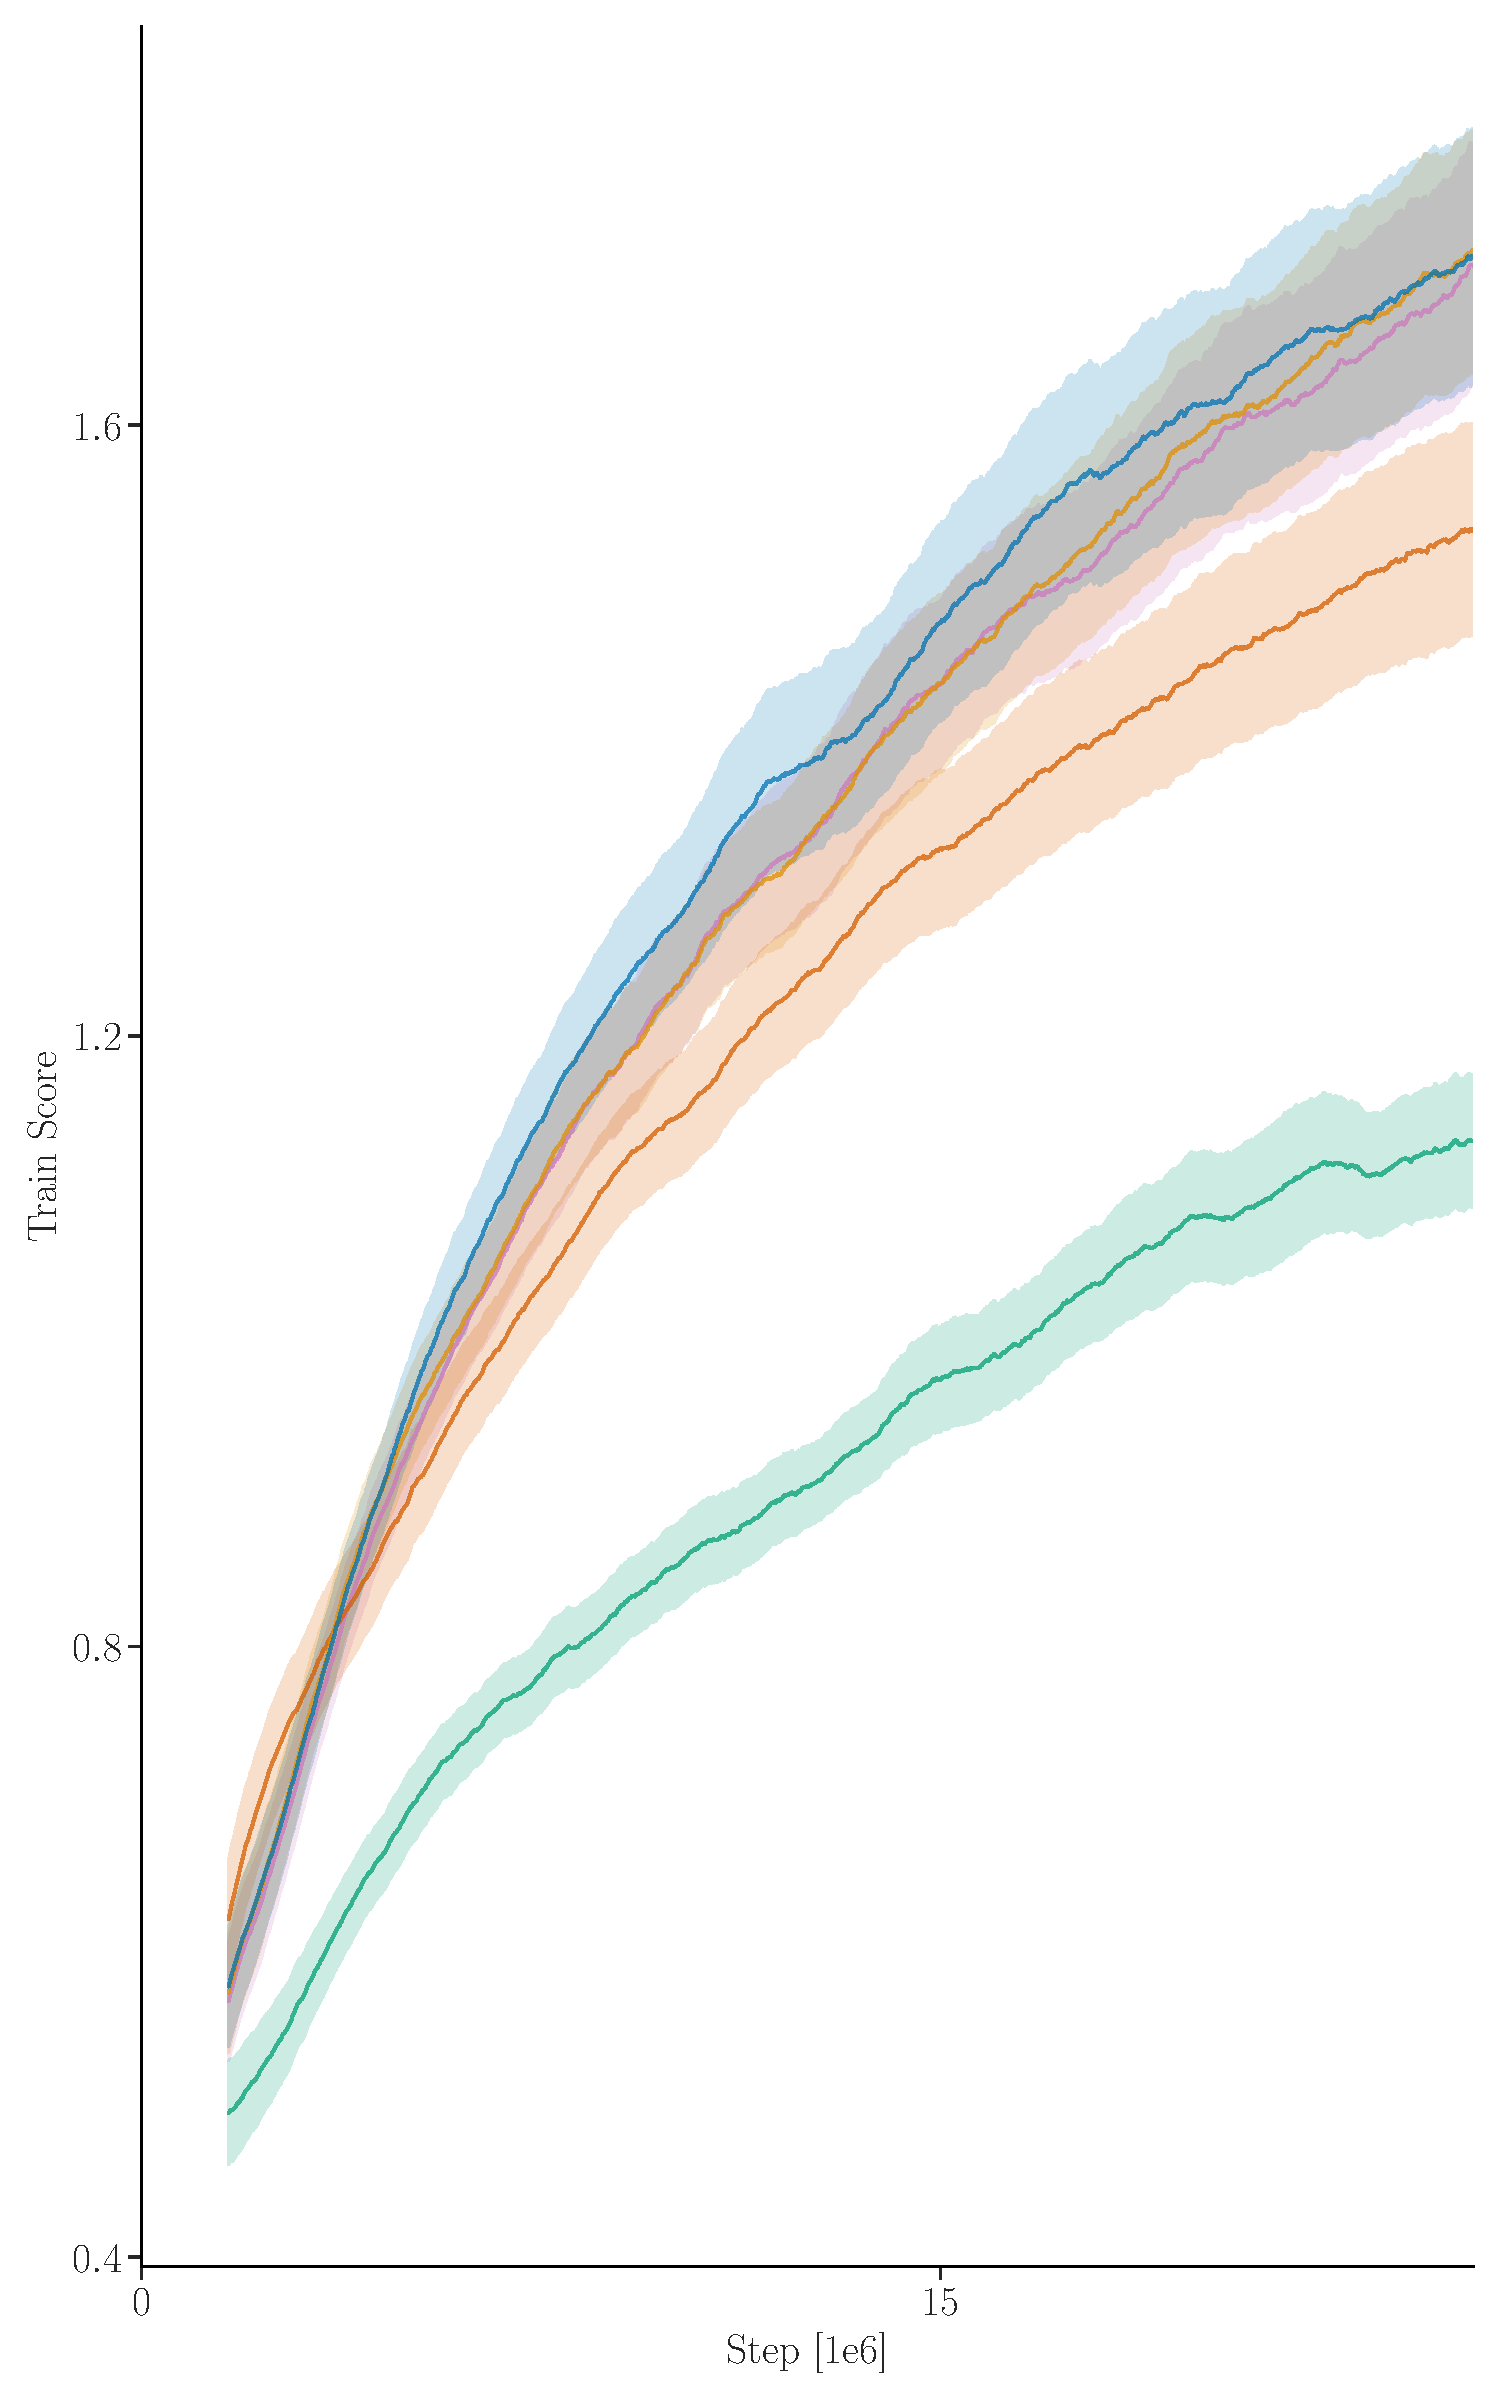
\includegraphics[width=1\linewidth]{app_content/procgen/trainset_curves_all_env.pdf}
            \caption{Train Score}\label{subfig:procgen_agg_train}
    \end{subfigure}%
        \begin{subfigure}{0.33\linewidth}
            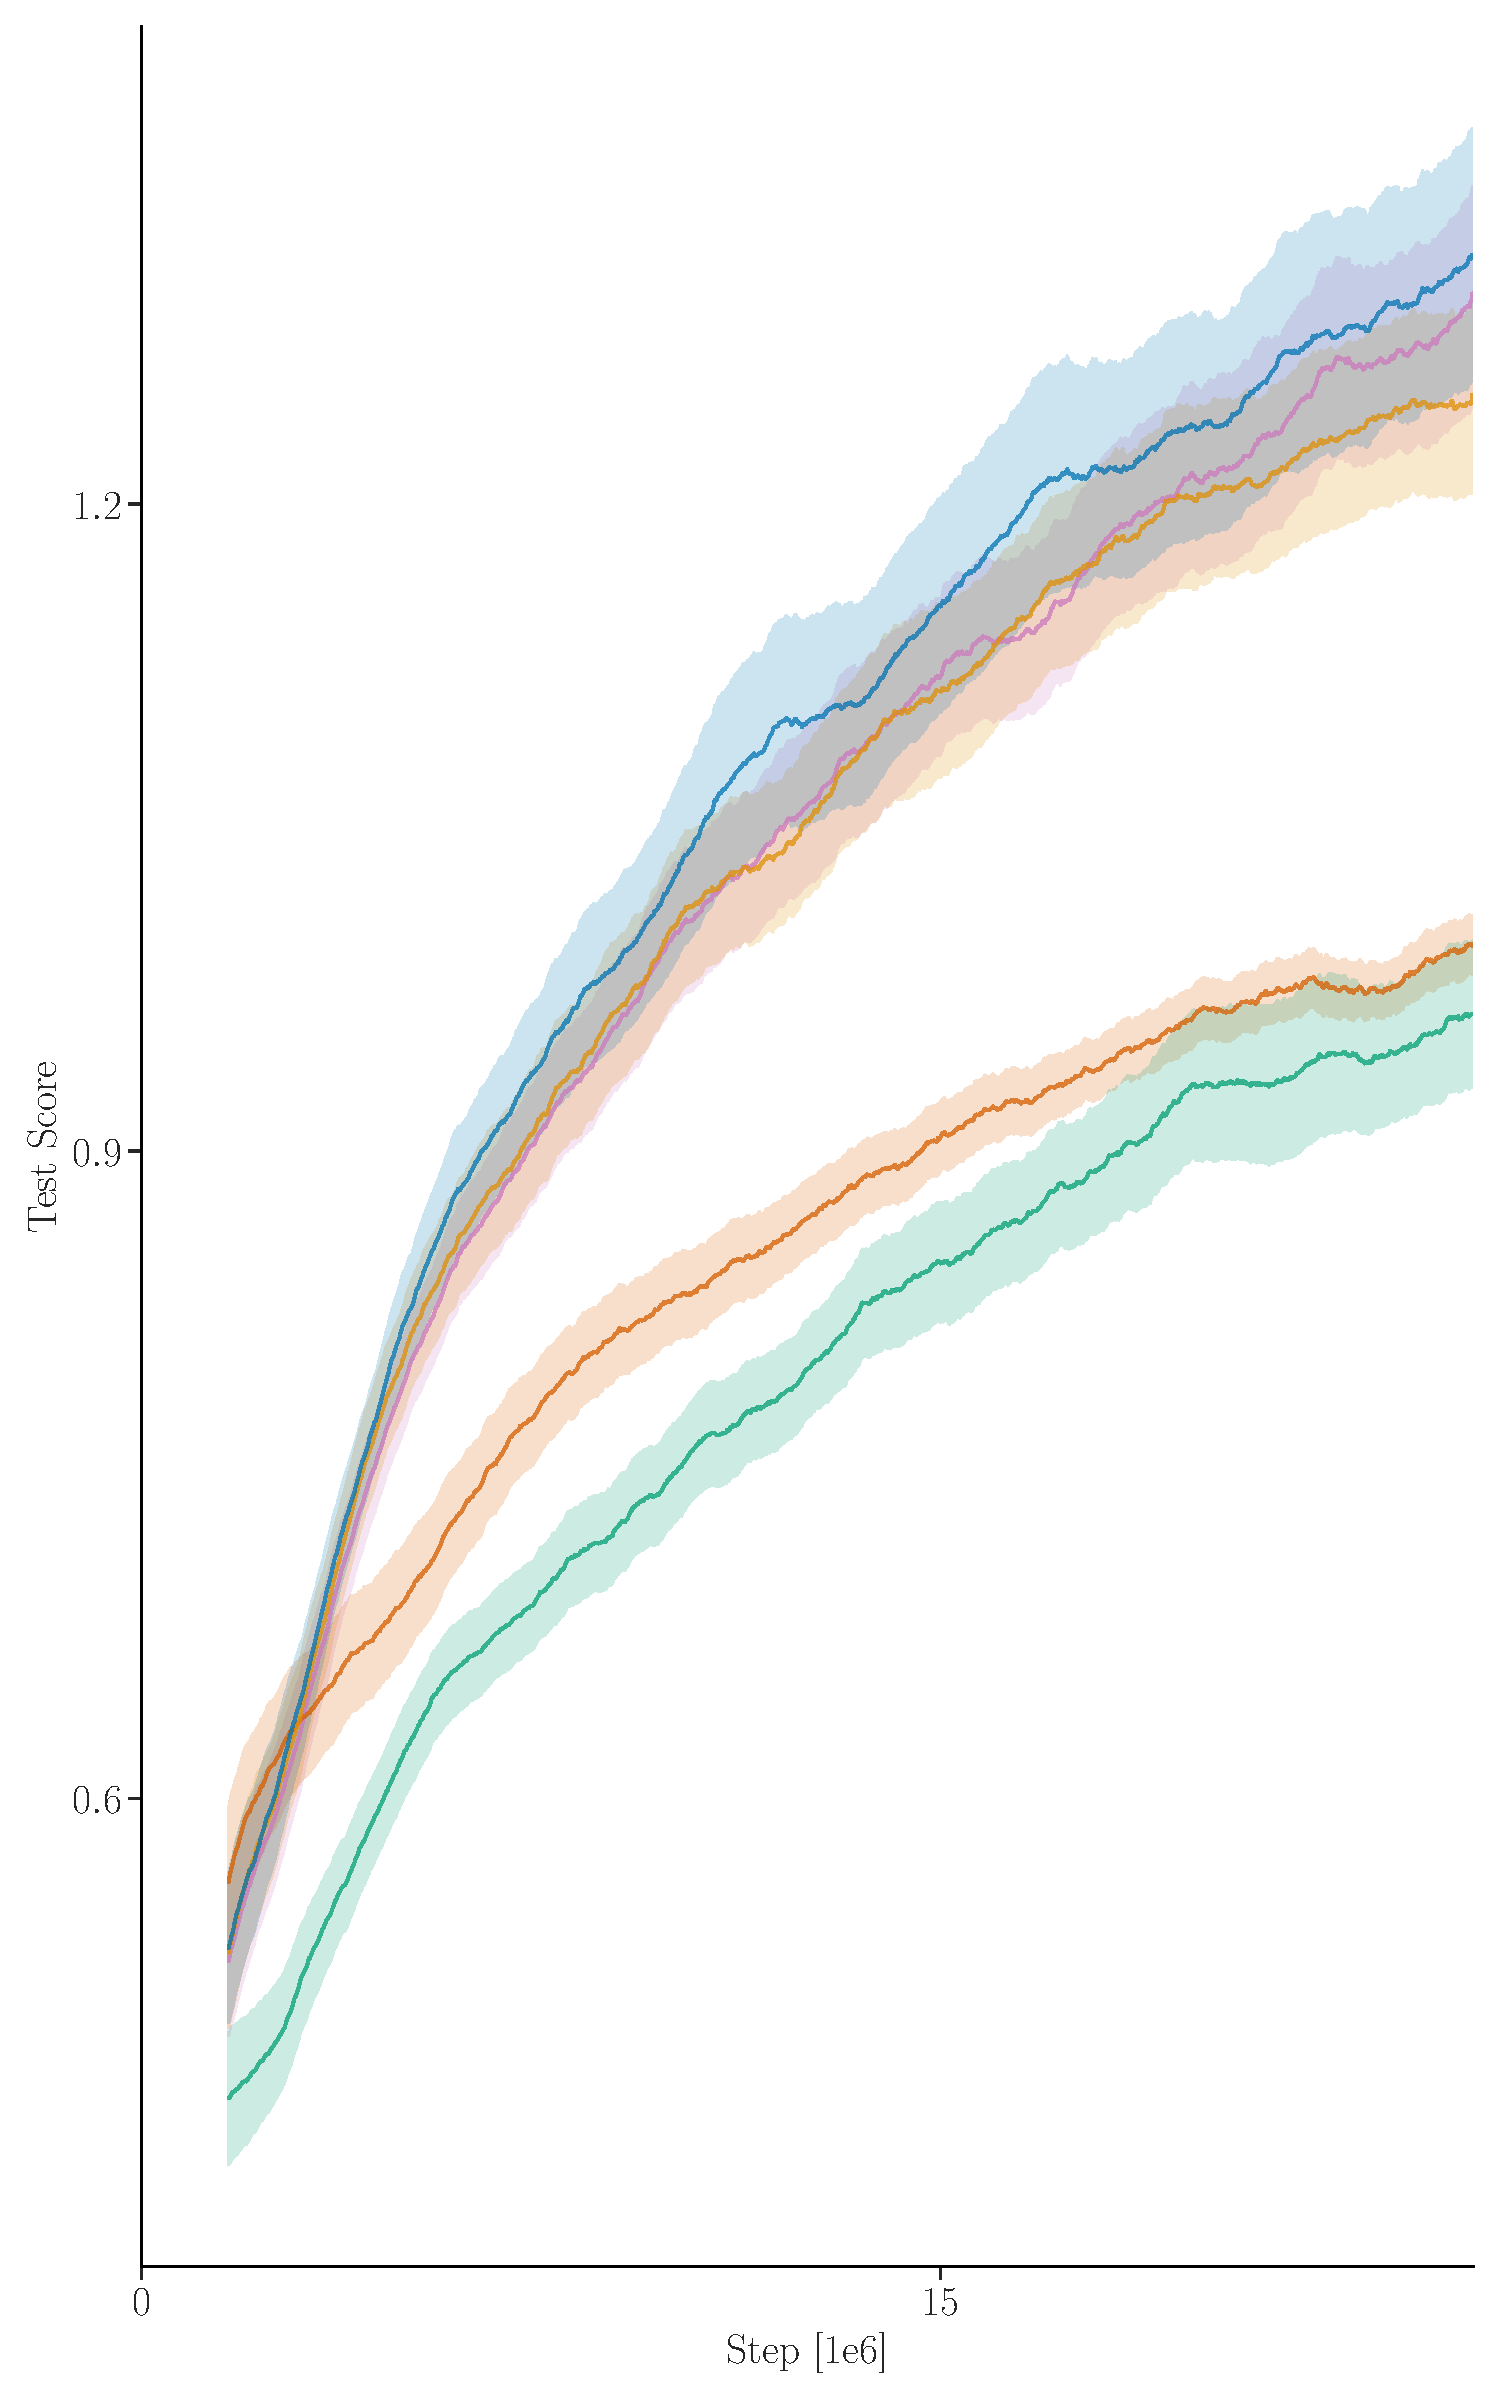
\includegraphics[width=1\linewidth]{app_content/procgen/testset_curves_all_env.pdf}
            \caption{Test Score}\label{subfig:procgen_agg_test}
    \end{subfigure}%
    \begin{subfigure}{0.33\linewidth}
            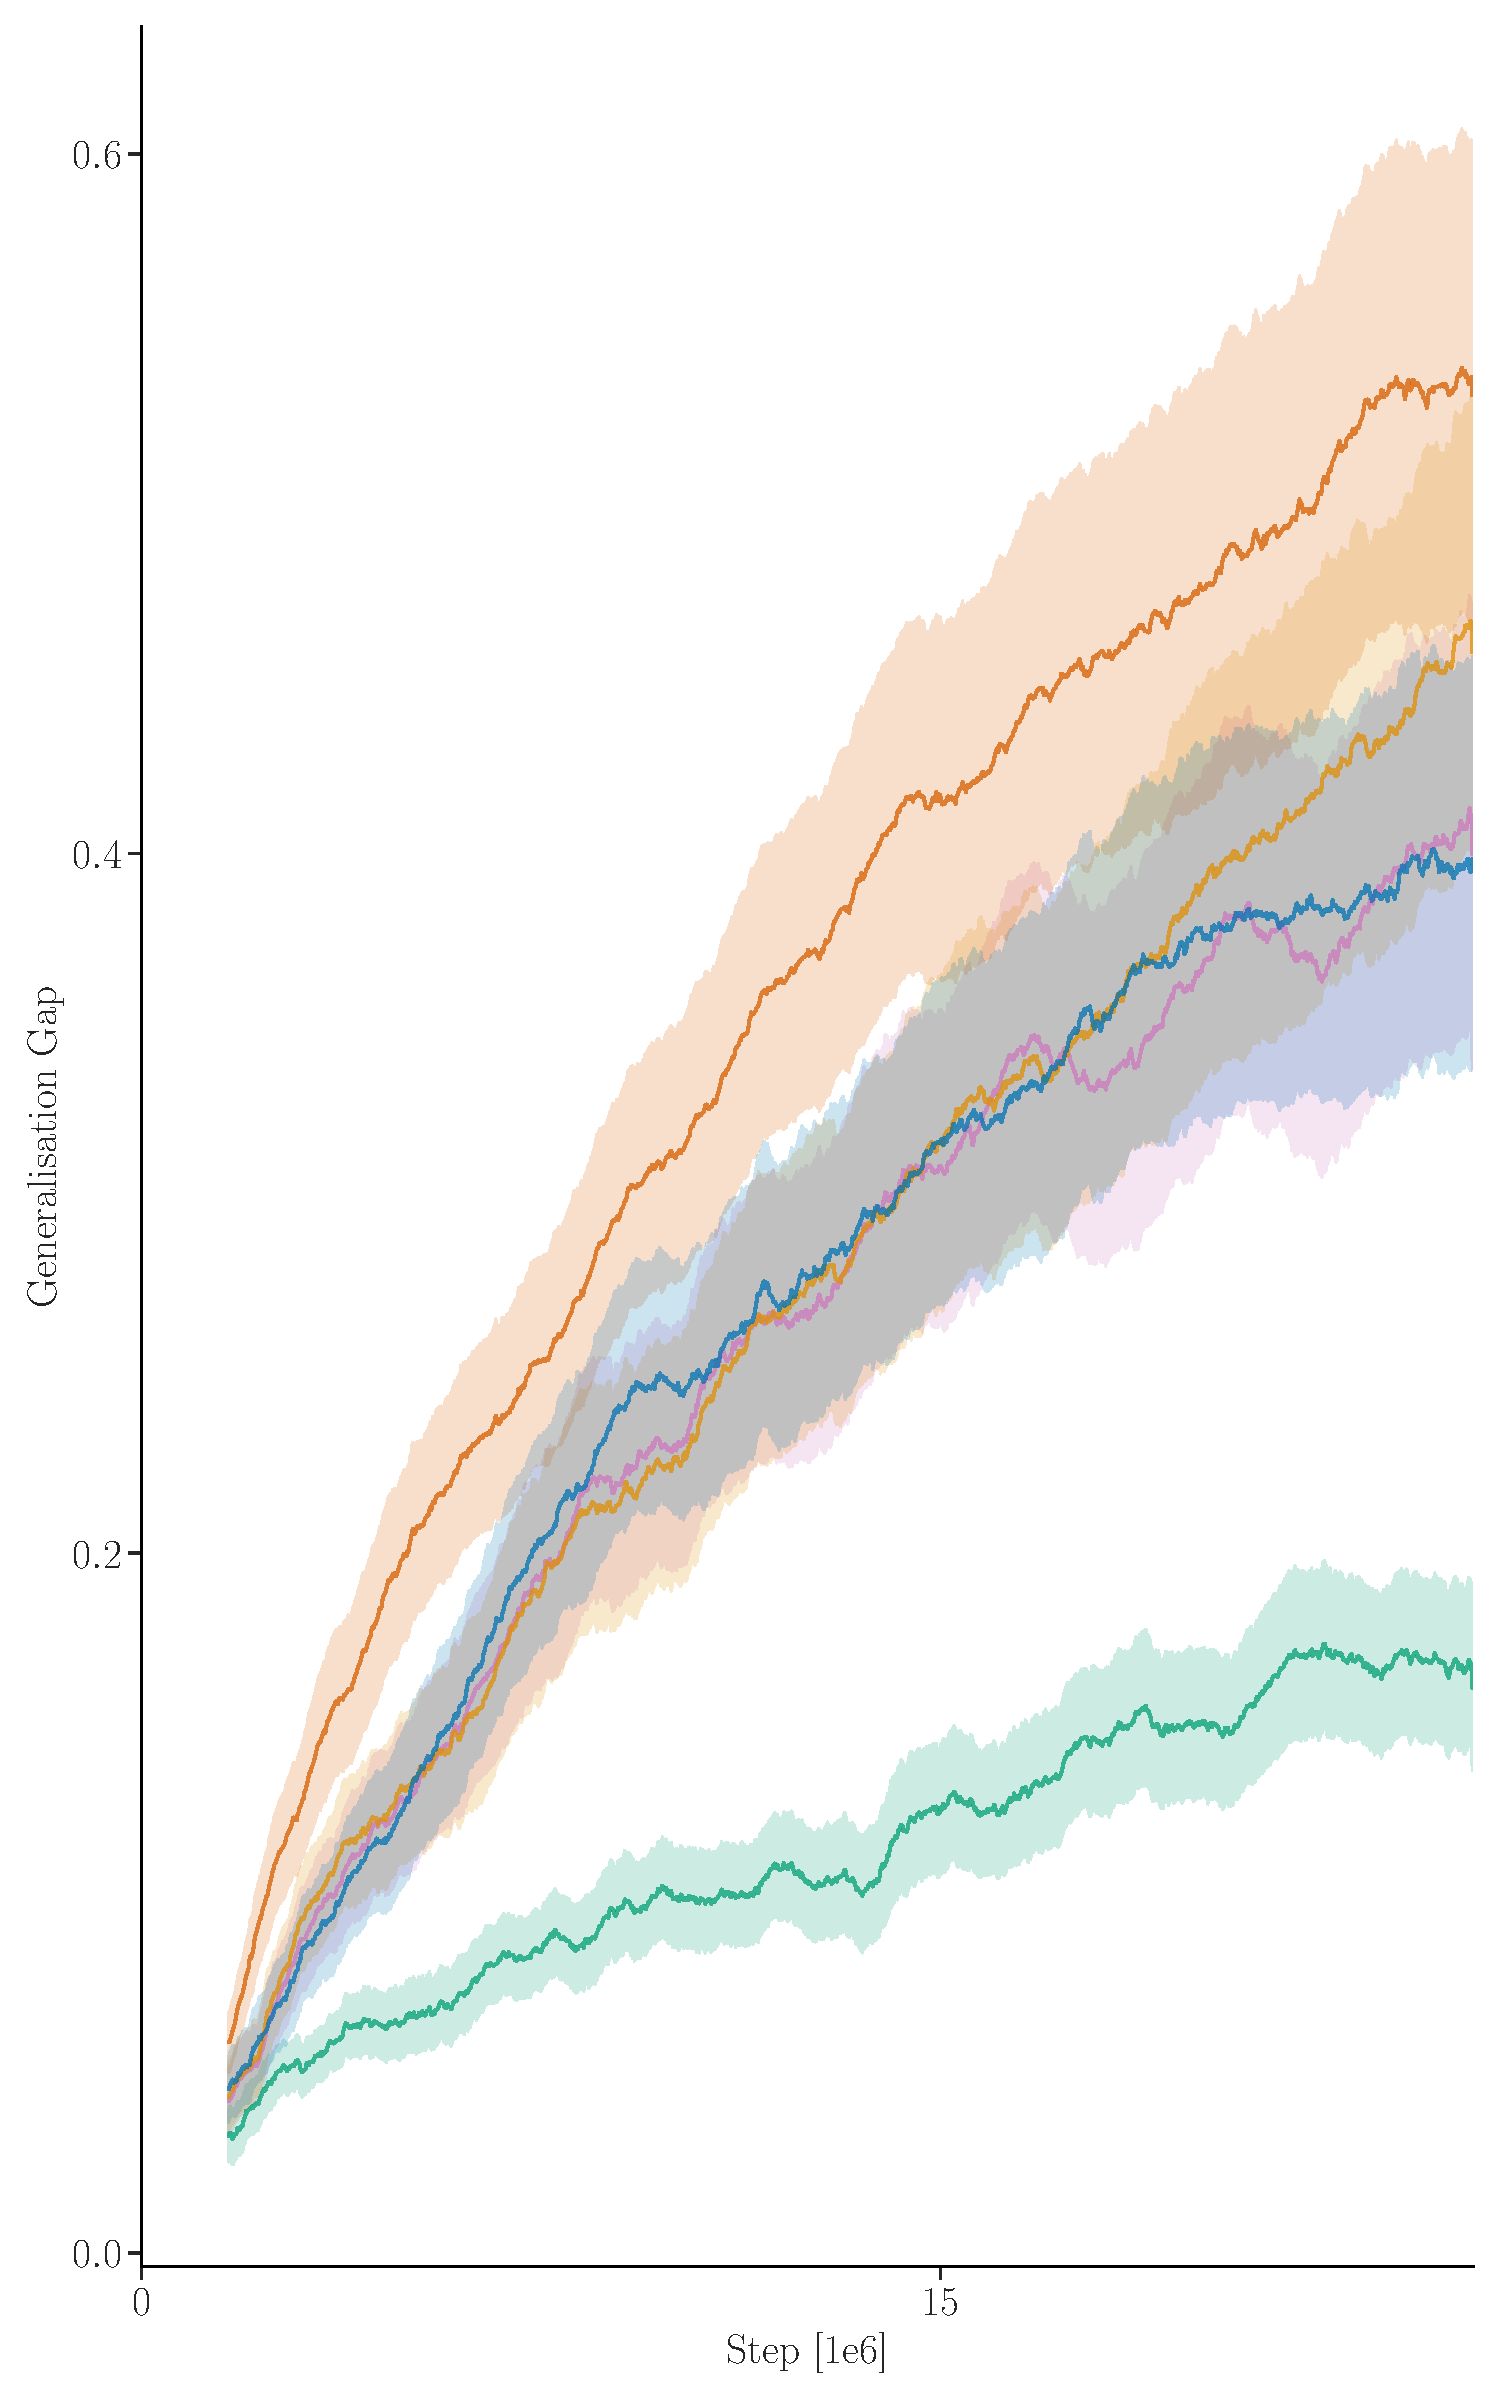
\includegraphics[width=1\linewidth]{app_content/procgen/gengap_curves_all_env.pdf}
            \caption{Generalisation Gap}\label{subfig:procgen_agg_gengap}
    \end{subfigure}
    \caption{Procgen normalised scores across environments and generalisation gap over the course of training.
    }
    \label{fig:procgen_agg_train_test_curves}
\end{figure}

\begin{figure}[H]
    \centering
    
\includegraphics[width=1\linewidth]{app_content/procgen/trainset_curves_per_env_legend.pdf}
    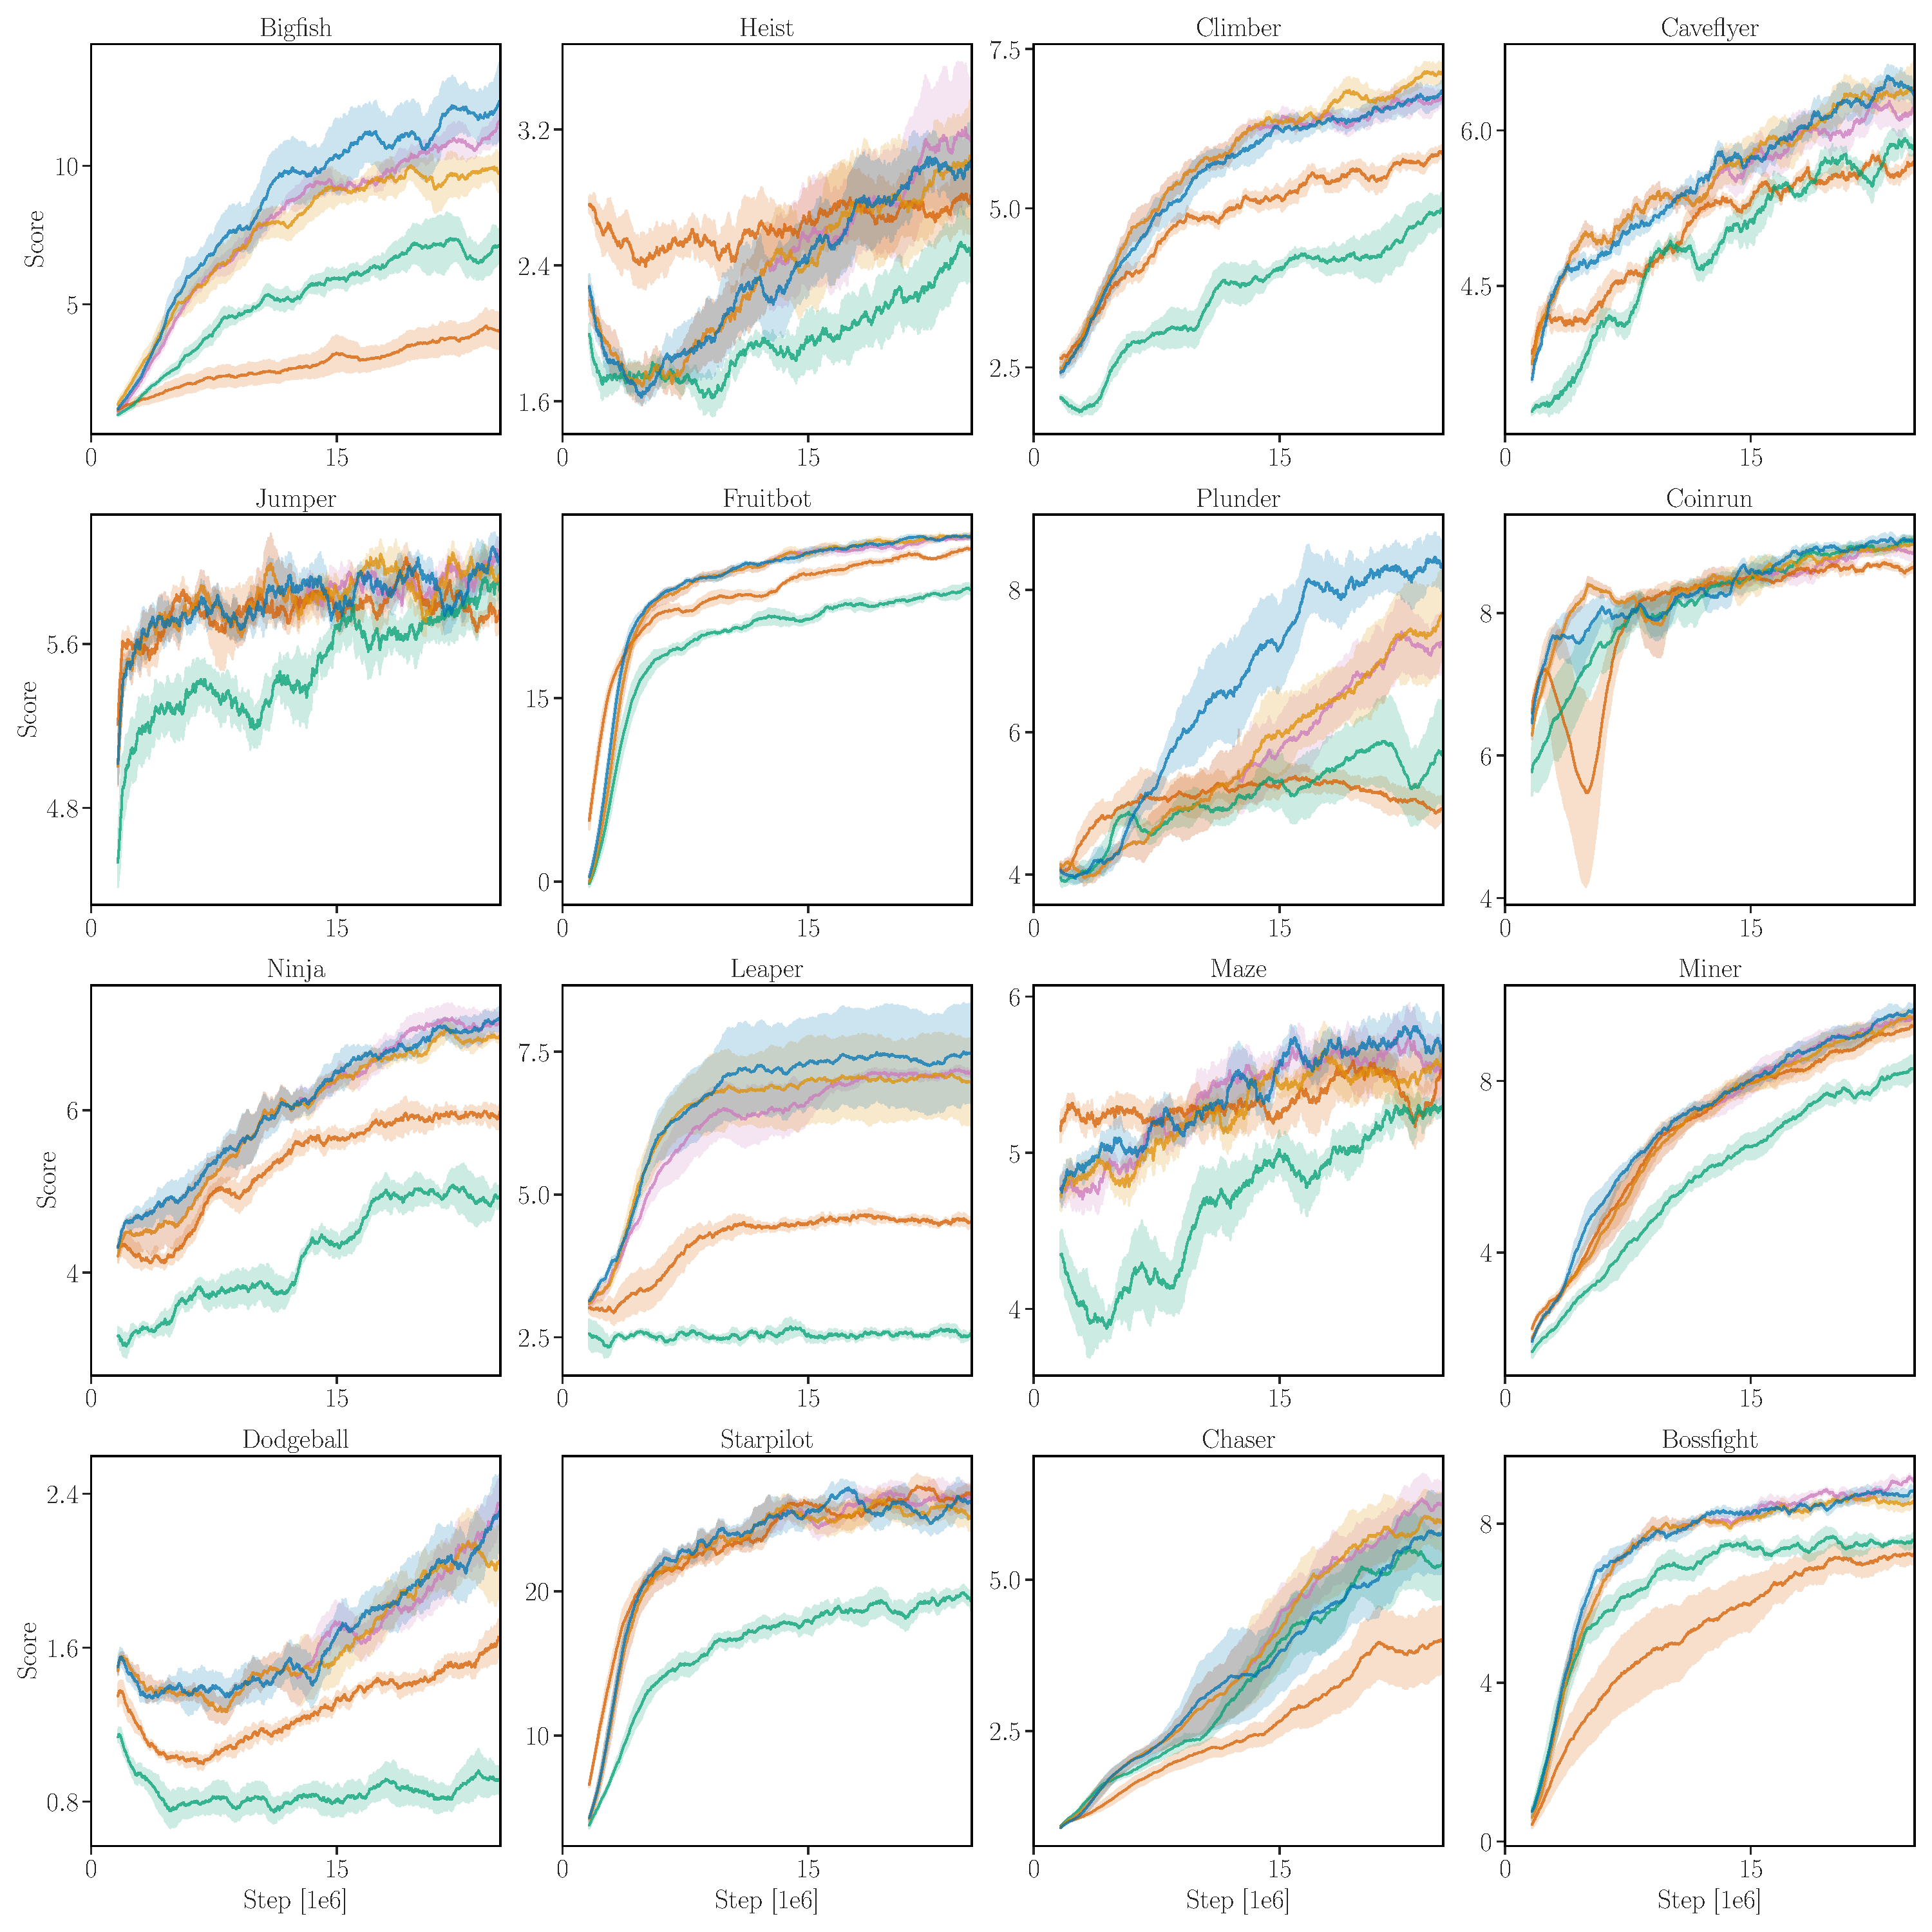
\includegraphics[width=1\linewidth]{app_content/procgen/testset_curves_per_env.pdf}
    \caption{Procgen per game test set scores over the course of training.
    }
    \label{fig:procgen_perenv_test_curves}
\end{figure}

\begin{figure}[H]
    \centering
    
\includegraphics[width=1\linewidth]{app_content/procgen/trainset_curves_per_env_legend.pdf}
    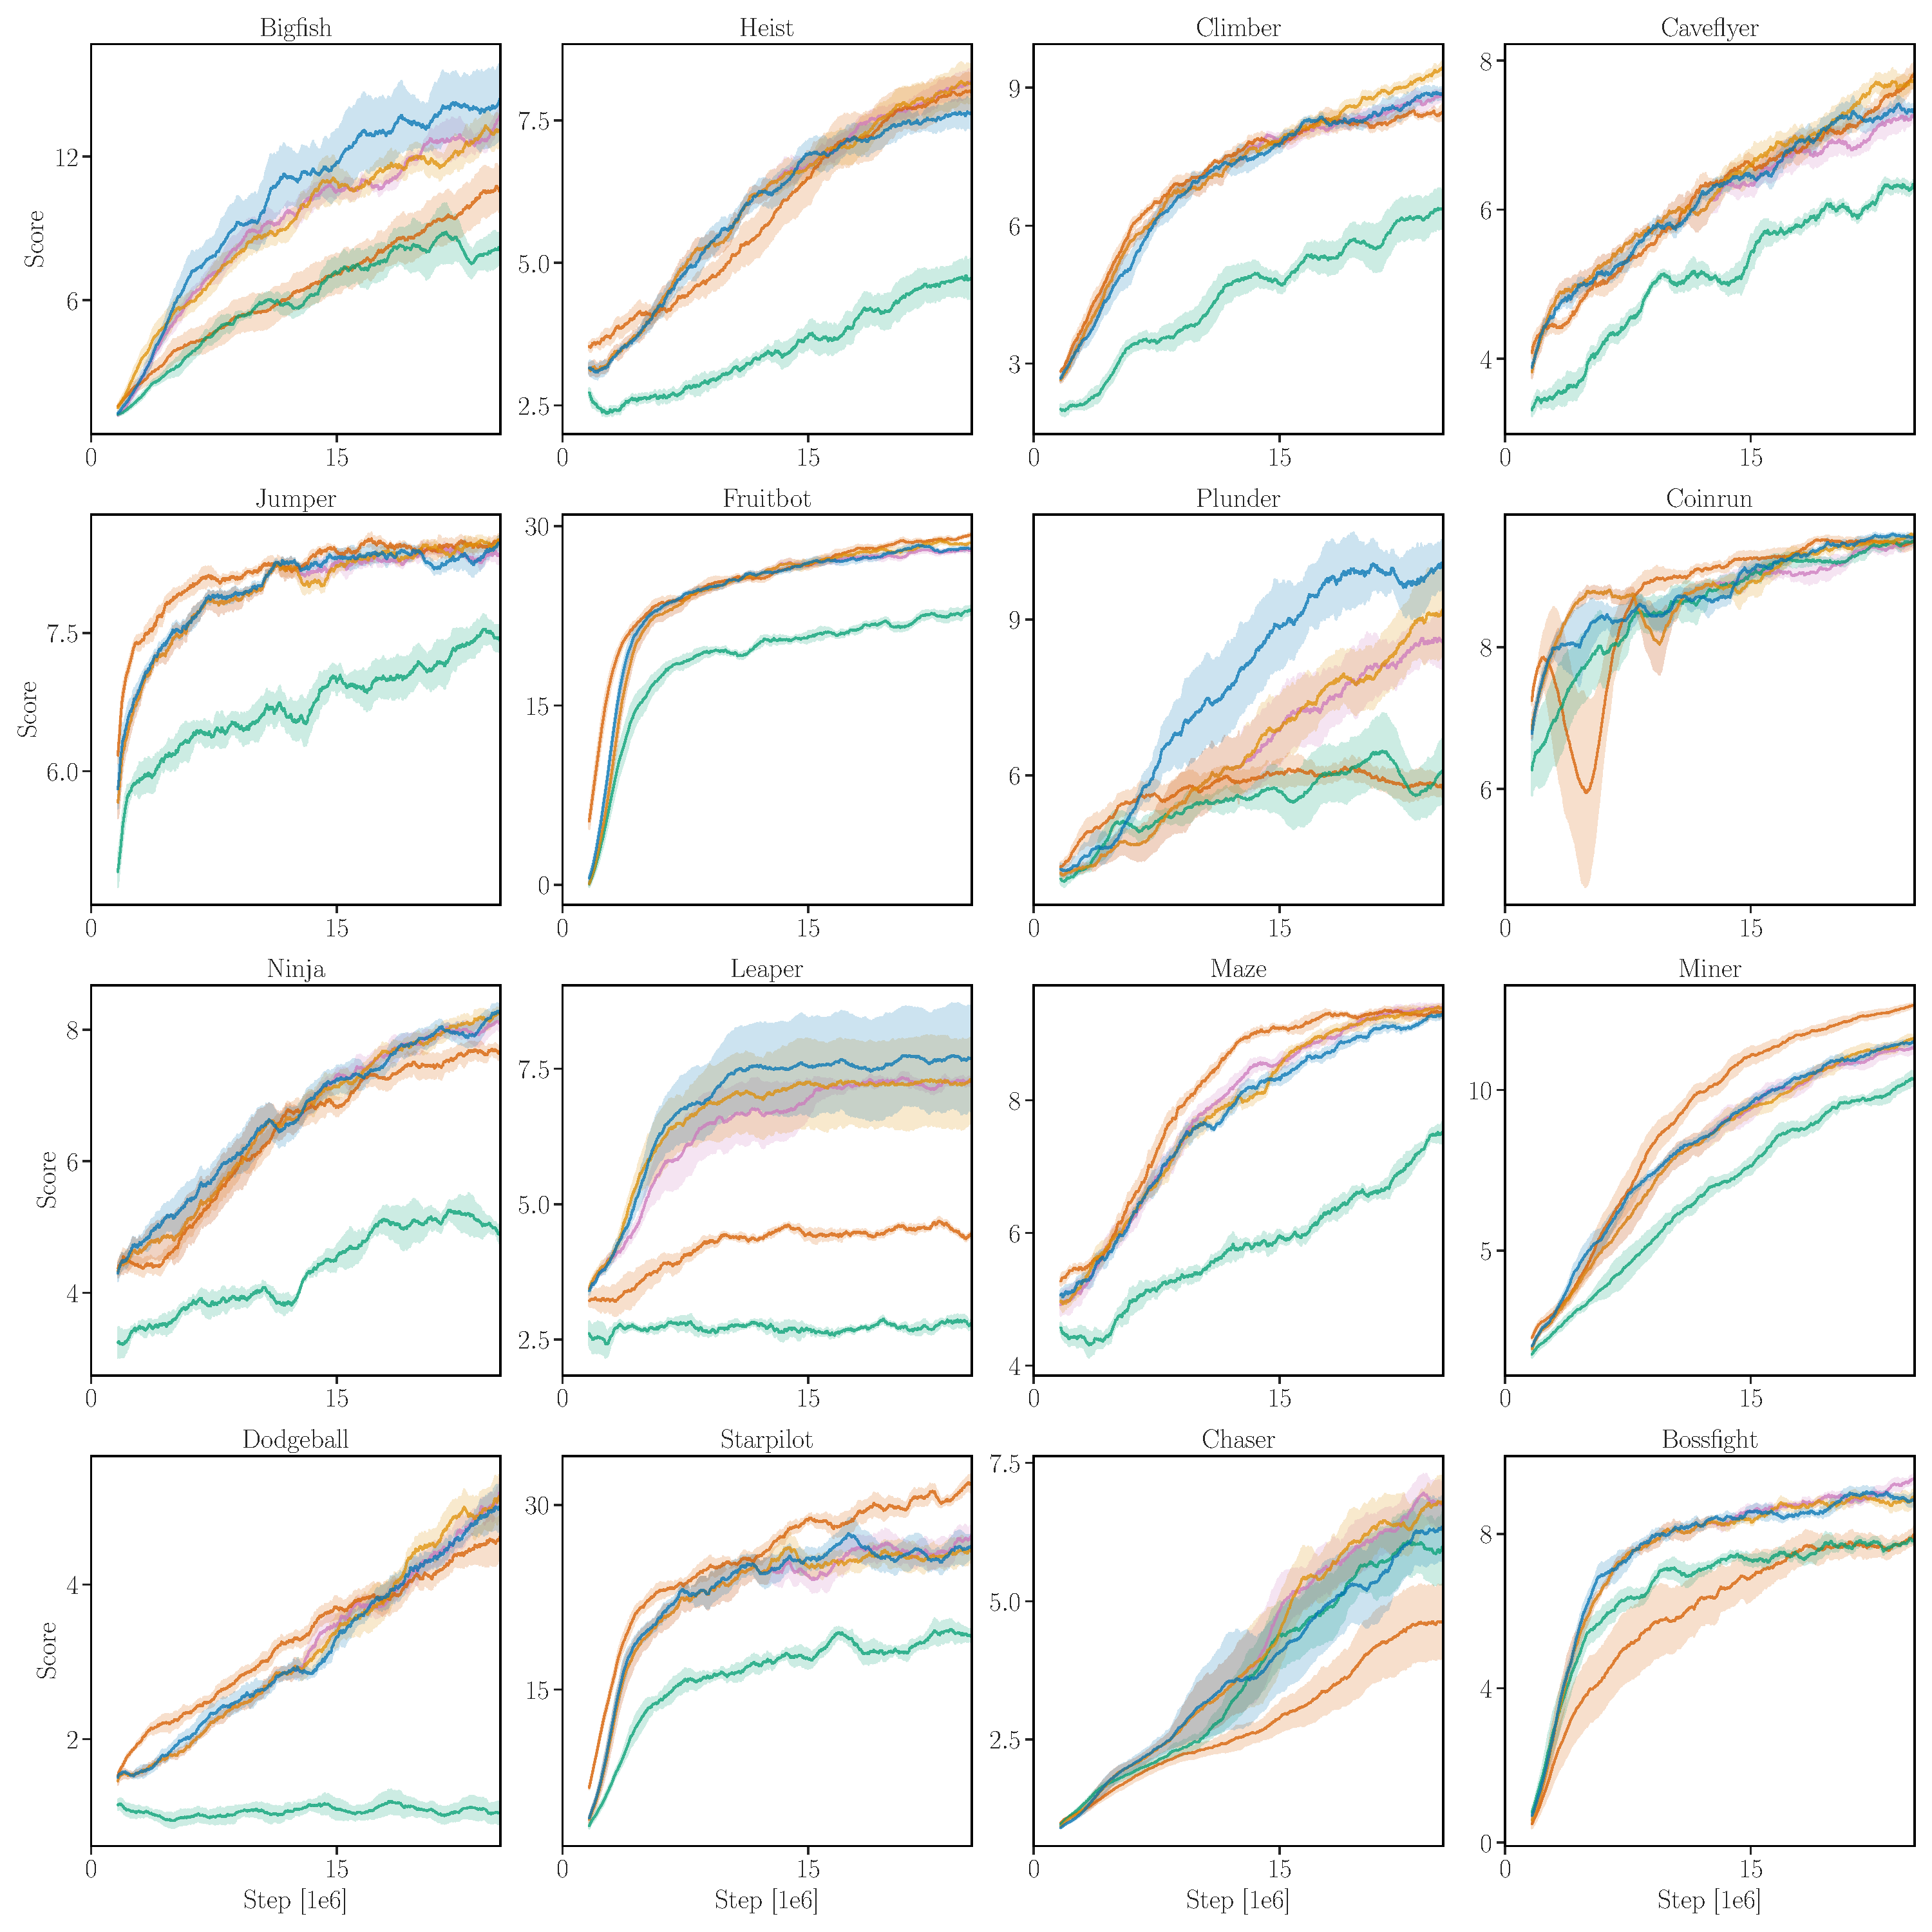
\includegraphics[width=1\linewidth]{app_content/procgen/trainset_curves_per_env.pdf}
    \caption{Procgen per game train set scores over the course of training.
    }
    \label{fig:procgen_perenv_train_curves}
\end{figure}


%Dropped:
%TODO: make distinction between estimated cross-entropy and true information. (in last section: it is therefore possible to approximate MI up to a constant using the cross-entropy of a classifier trained to predict i from z.
%We estimate $\mut(L, b)$ for all methods tested, finding that our mutual information estimate strongly correlates with the generalisation gap across all procgen games and methods tested, with Kendall rank correlation coefficient $\tau=0.41$ ($p<1\mathrm{e}{-33}$). %DROPPED: should we introduce kendall coeff? is it the right spot to provide this information?

%We find these numbers surprising, given that the classifier makes a prediction from an internal observation obtained from a single observation, as the agent architecture is non-recurrent.  

% In \cref{fig:procgen_results}, we compare our method to the $S^V$ $\ell_1$-value loss scoring strategy, using the same hyperparameters as the original implementation \citep{PLR}
%---------------------
%TODO add result tables
\section{Minigrid additional experimental results}\label{app:results_minigrid}

\subsection{Quantifying the distributional shift in minigrid}\label{app:dist-shift}

%TODO: figures update overgernarlisation -> Shift induced gap
In \Cref{fig:gen_gaps}, we report the $\text{GenGap}$ and the $\text{ShiftGap}$ in the Minigrid experiments. The $\text{GenGap}$ is not helpful in interpreting the poor test set performance of UED methods. In fact, we report in \Cref{fig:minigrid_train_curves} that UED methods tend to perform well when evaluated on levels sampled from $P_\Lambda$, while performing poorly on the train and test sets. This results in the $\text{GenGap}$ remaining close to zero throughout training. 

We would also expect the $\text{GenGap}$ and the train and test scores to be near-zero for a random policy, that is if the agent was not learning anything at all. However ACCEL and RPLR experience a different failure mode: the UED-trained agents are learning, as demonstrated by their scores on their respective training distributions, but they are learning to solve a different CMDP. In contrast, the $\text{ShiftGap}$ is effective at distinguishing between the agent not learning at all and it learning an out-of-context policy.
%This type of misgeneralisation shares some similarity with \textit{goal misgeneralisation} \cite{goal_misgen_DRL,goal_misgen_deepmind}, a phenomenon in which the agent learns to optimise the wrong objective. This objective is usually indistinguishable from the intended objective during training (i.e. yields similar returns), but results in much lower returns and/or undesired behavior at deployment. In our case, misgeneralisation is not induced by the agent learning a different behaviour that is indistinguishable from the desired behaviour under  but indirectly, through an induced shift in the training distribution   

While the $\text{ShiftGap}$ allows us to quantify how the distributional shift impacts the agent performance, we desire to quantify the distributional shift directly, and within a feature space consistent with the CMDP semantics. We first compute the distribution $c(t,d|i_{\vx})$, the probability of tile type $t$ occurring at shortest path $d$ from the goal location, for each level $i_{\vx} \in \Lambda$. $c_p$ is the marginal $c_p = \mathbb{E}_{i_{\vx} \sim p(i_{\vx})}[c(t,d|i_{\vx})]$ and we measure the Jensen-Shannon Divergence $\text{JSD}(c_p||c_q)$, with $p=P_\Lambda$ and $q=\mathcal{U}(X_\text{train})$.

\begin{figure}[!htb]
    \centering
    
\includegraphics[width=1\linewidth]{app_content/all-legend.pdf}
    \begin{subfigure}{0.49\linewidth}
            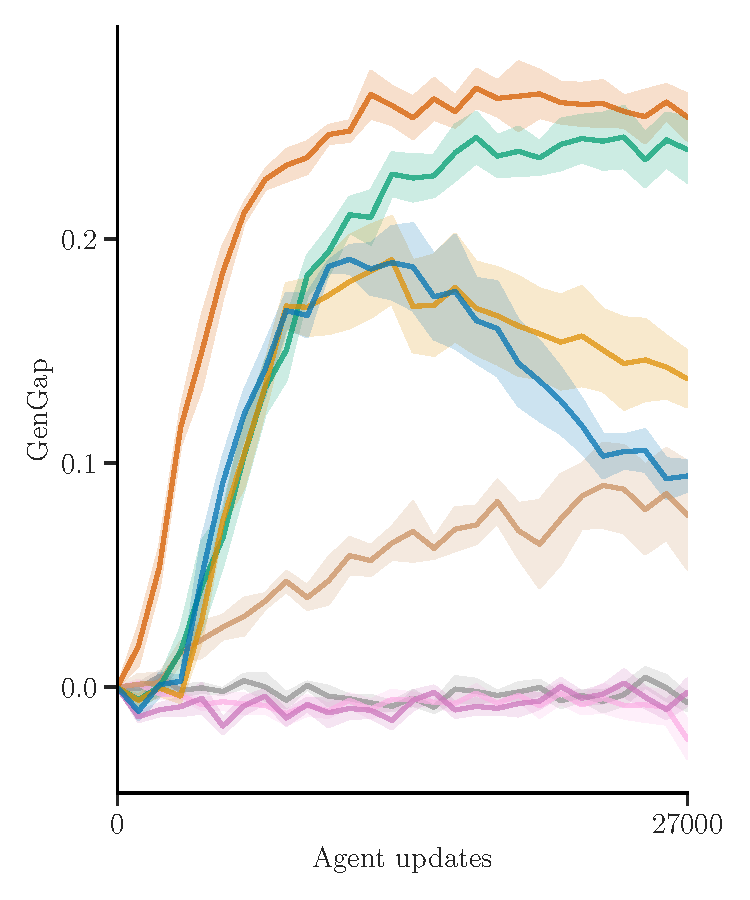
\includegraphics[width=1\linewidth]{app_content/gen_gaps/gengap-all.pdf}
            \caption{}\label{subfig:gengap}
    \end{subfigure}%
        \begin{subfigure}{0.49\linewidth}
            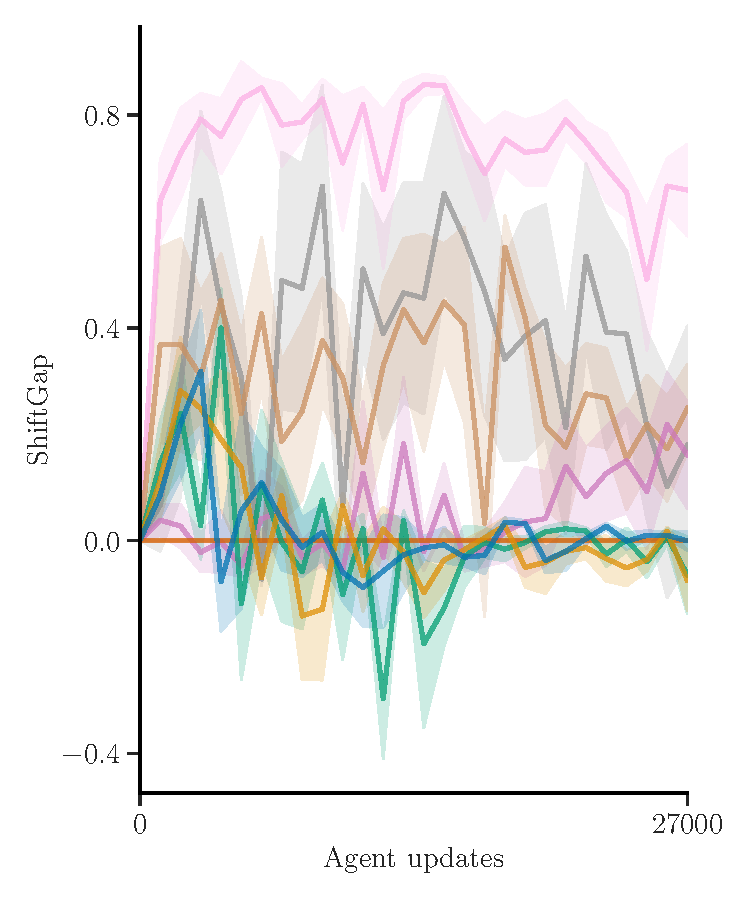
\includegraphics[width=1\linewidth]{app_content/gen_gaps/shiftgap-all.pdf}
            \caption{}\label{subfig:overgengap}
    \end{subfigure}%
    \caption{Evolution of (a) the $\text{GenGap}$ (\Cref{eq:GenGap}) and (b) the $\text{ShiftGap}$ (\Cref{eq:ShiftGap}) over the course of training. Fixed set sampling strategies experience higher $\text{GenGap}$ and low $\text{ShiftGap}$, while UED methods follow the opposite trend. Both DRED methods maintain near-zero $\text{ShiftGap}$ while achieving a significantly smaller $\text{GenGap}$ than fixed set strategies. DR spends the majority of training with a low $\text{GenGap}$ and $\text{ShiftGap}$, but a sharp increase towards the end of training brings its $\text{ShiftGap}$ to similar levels as RPLR and ACCEL-D.
    }
    \label{fig:gen_gaps}
\end{figure}

We report how the JSD evolves over the course of training for different methods in \Cref{subfig:jsd}. We observe that distributional shift occurs early on during training and remains relatively stable afterwards in all methods. Surprisingly, both DRED methods demonstrate a smaller JSD than PLR, even though PLR only samples $X_\text{train}$ levels. JSD and ShiftGap are positively correlated for all methods except DR and PLR, which both present high JSD but low ShiftGap. VAE-DRED is the only generative method to maintain a low JSD and ShiftGap throughout training. Interestingly, and with the exception of $\mathcal{U}$, methods rank nearly identically to their test set performance ranking when sorted according to their JSD (lowest first). This relationship appears to hold throughout training, as can be observed by comparing the JSD with $X_\text{test}$ scores in \Cref{fig:minigrid_train_curves}.%, which can be visually observed by comparing levels generated using different methods in \Cref{fig:generated_levels}. %TODO: fig with generated levels

In \Cref{fig:buffermetrics}, we report additional metrics on the levels sampled by each method. Over the course of training, only VAE-DRED and PLR stay relatively consistent with $X_\text{train}$ across the three metrics considered.

\begin{figure}[!htb]
    \centering
    
\includegraphics[width=1\linewidth]{app_content/all-legend.pdf}
    \begin{subfigure}{0.49\linewidth}
            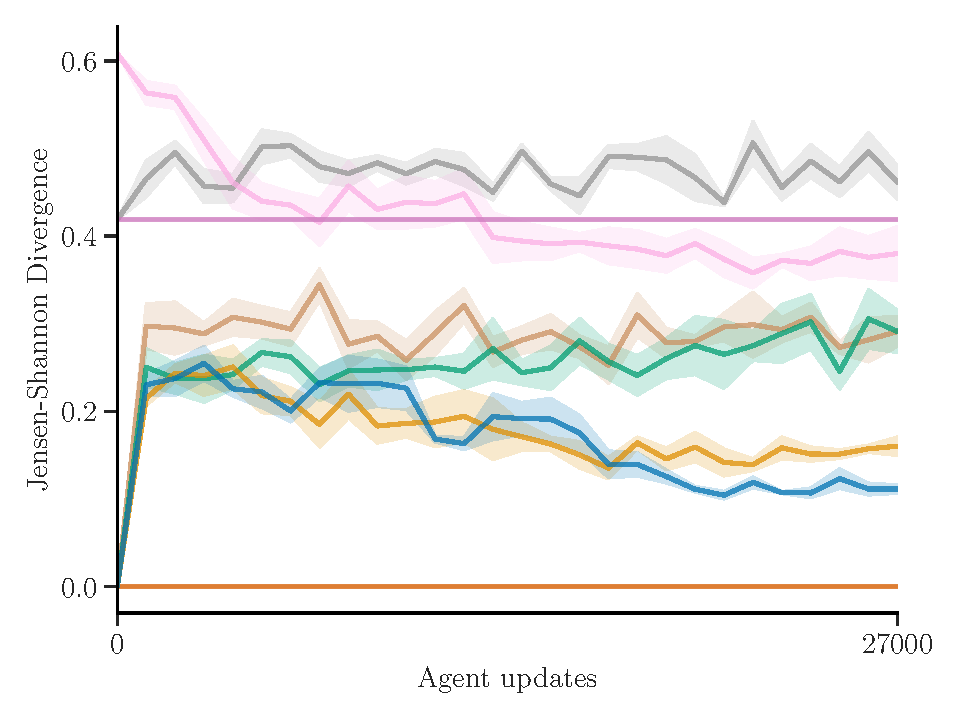
\includegraphics[width=1\linewidth]{app_content/buffer_metrics/jsd-all.pdf}
            \caption{}\label{subfig:jsd}
    \end{subfigure}%
        \begin{subfigure}{0.49\linewidth}
            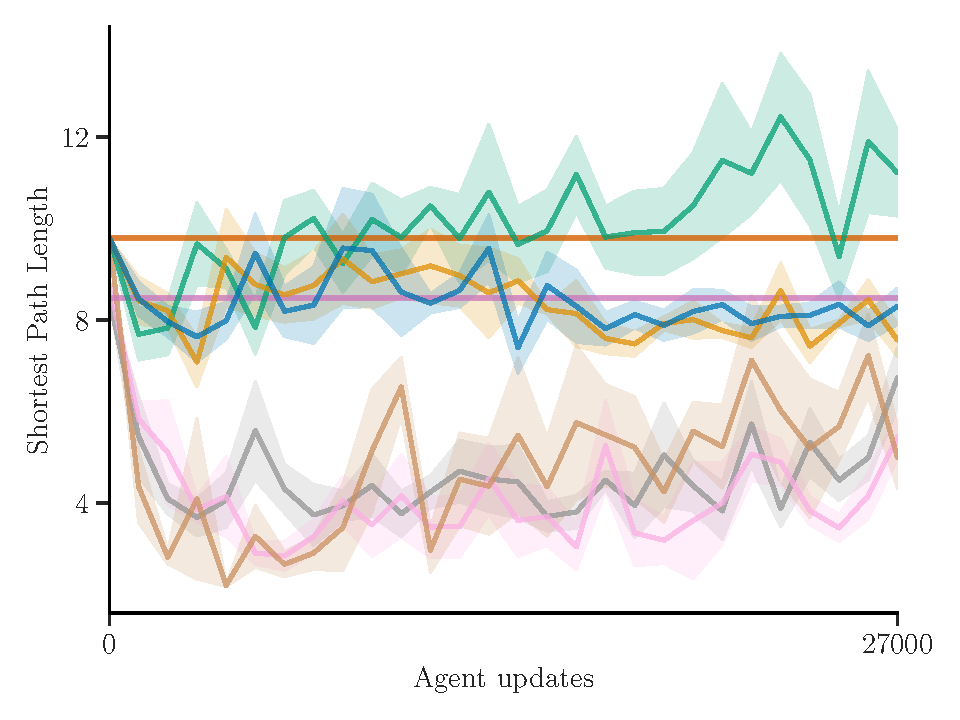
\includegraphics[width=1\linewidth]{app_content/buffer_metrics/shortest_path_lengthall.pdf}
            \caption{}
    \end{subfigure}\\
        \begin{subfigure}{0.49\linewidth}
            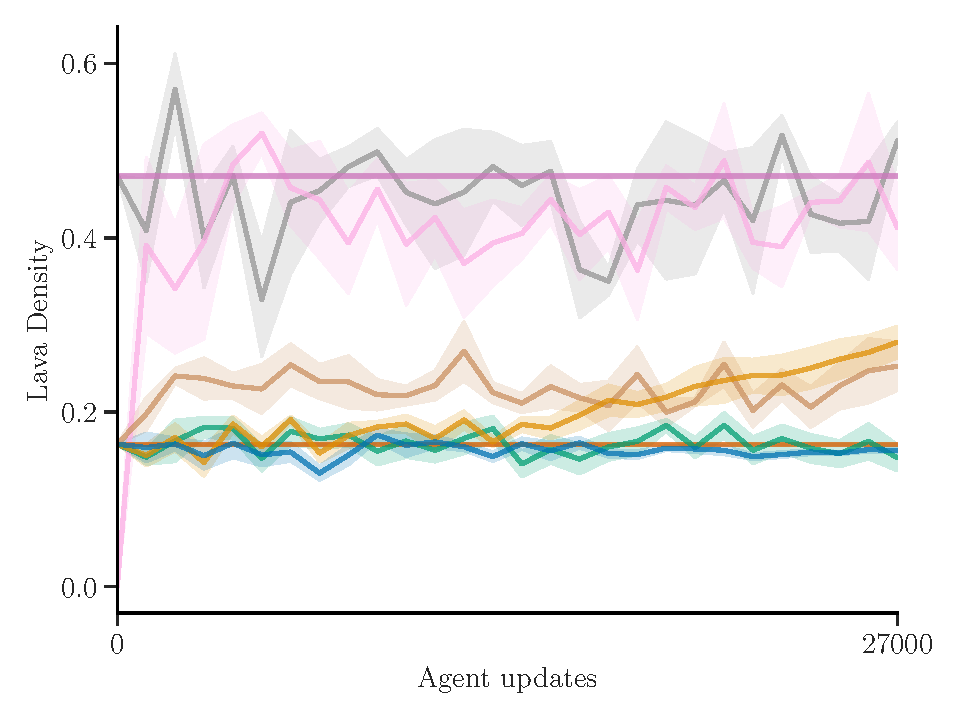
\includegraphics[width=1\linewidth]{app_content/buffer_metrics/lava_densityall.pdf}
            \caption{}
    \end{subfigure}%
            \begin{subfigure}{0.49\linewidth}
            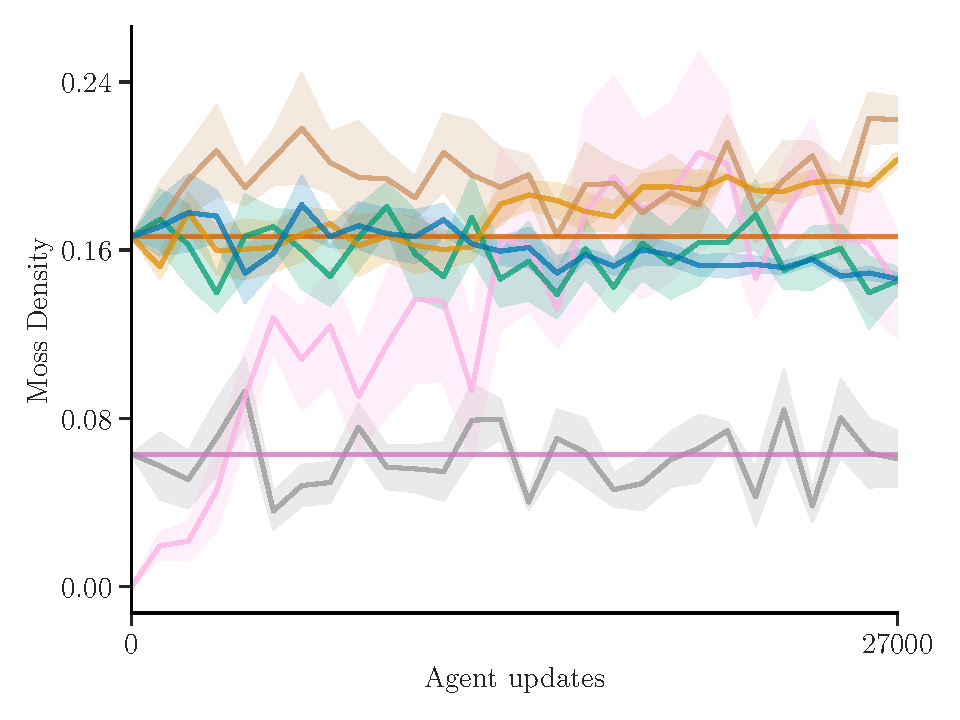
\includegraphics[width=1\linewidth]{app_content/buffer_metrics/moss_densityall.pdf}
            \caption{}
    \end{subfigure}%
    \caption{In sampled levels over the course of training, evolution of (a) the Jensen-Shannon divergence, (b) the shortest path length between the start and goal location, (c) the lava tile density (over non-navigable tiles) and (d) the moss tile density (over navigable tiles).}
    \label{fig:buffermetrics}
\end{figure}

\begin{figure}[H]
            
\includegraphics[width=1\linewidth]{app_content/all-legend.pdf}
    \begin{subfigure}{0.49\linewidth}
            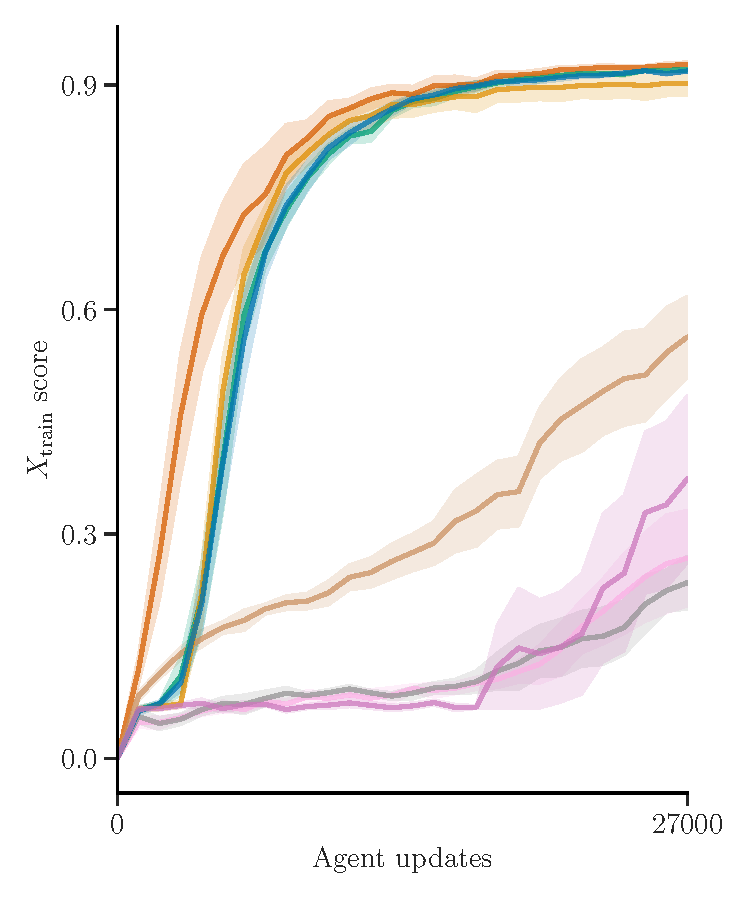
\includegraphics[width=1\linewidth]{app_content/minigrid_extra/train-scores_num_update.pdf}
    \end{subfigure}%
        \begin{subfigure}{0.49\linewidth}
            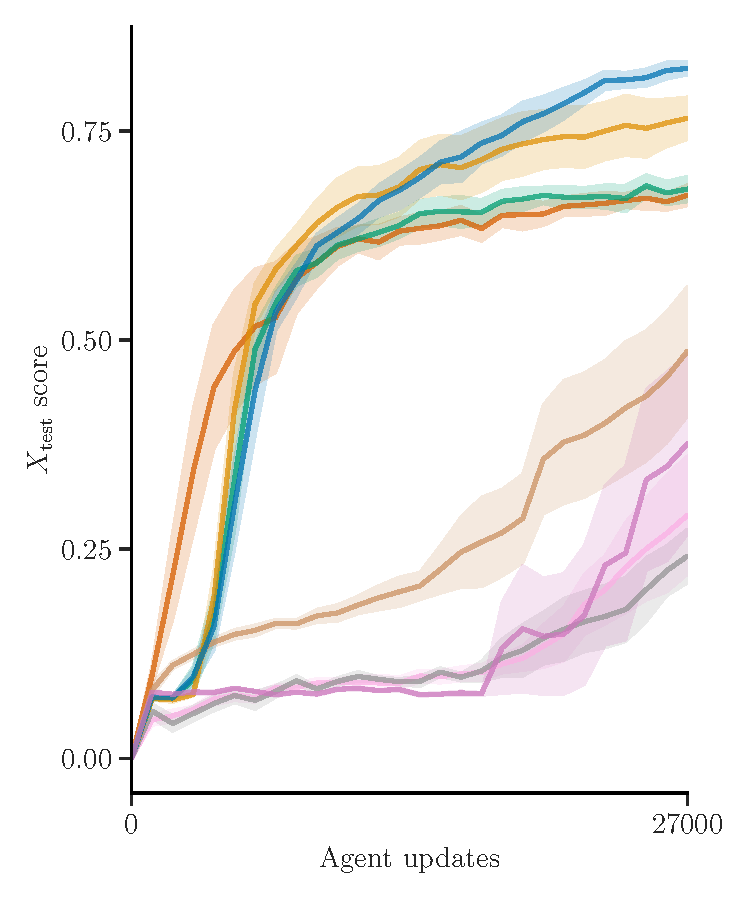
\includegraphics[width=1\linewidth]{app_content/minigrid_extra/test-scores_num_update.pdf}
    \end{subfigure}%
    \caption{Minigrid scores for $X_\text{train}$ and $X_\text{test}$ over the course of training. Shaded area represents the standard error across 5 seeds.
    }
    \label{fig:minigrid_train_curves}
\end{figure}

\subsection{Extended Minigrid results}\label{app:minigrid_extended_results}

\begin{figure}[H]
\centering%%%%%%%%%%%%%%%%%%%%%%%%%%%%%%%%%%%%%%%%%%%%%%%%%
    \begin{subfigure}[]{.08\linewidth}
    \centering
    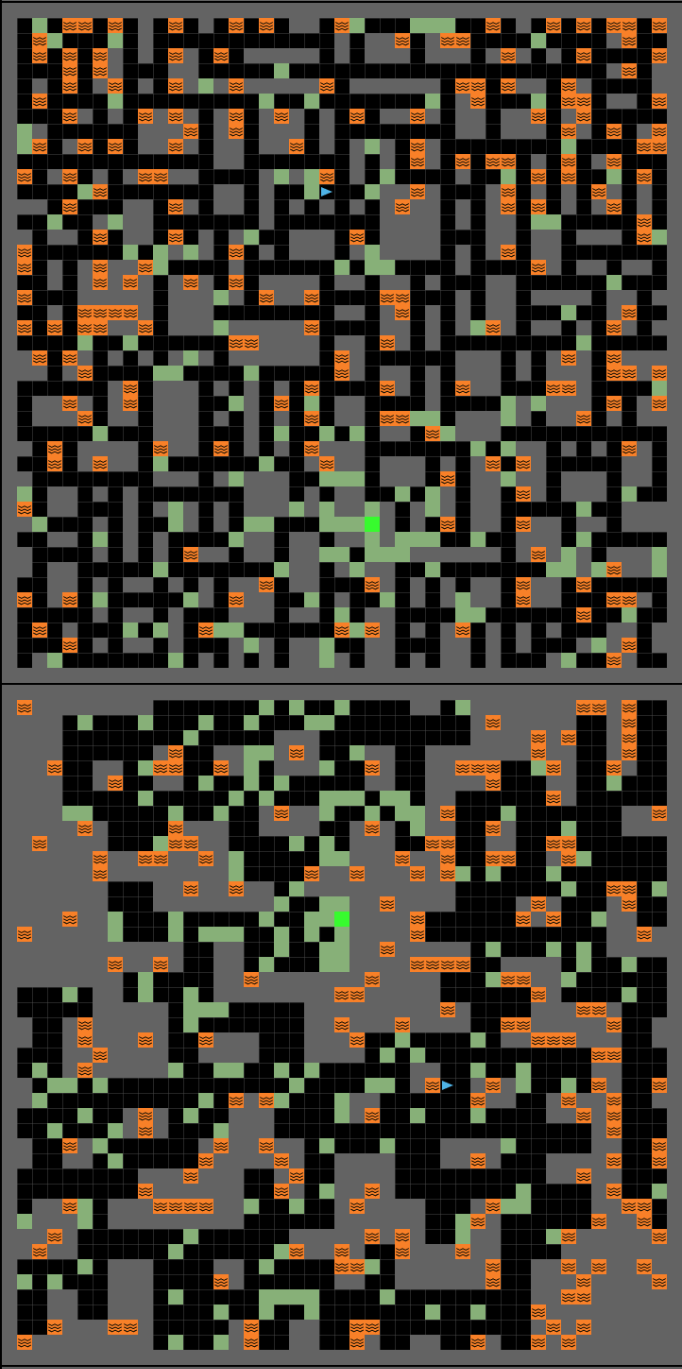
\includegraphics[width=1\linewidth]{content/layouts/large_layouts2x1.png}
  \end{subfigure}%
   \begin{subfigure}[]{.72\linewidth}
    \centering
    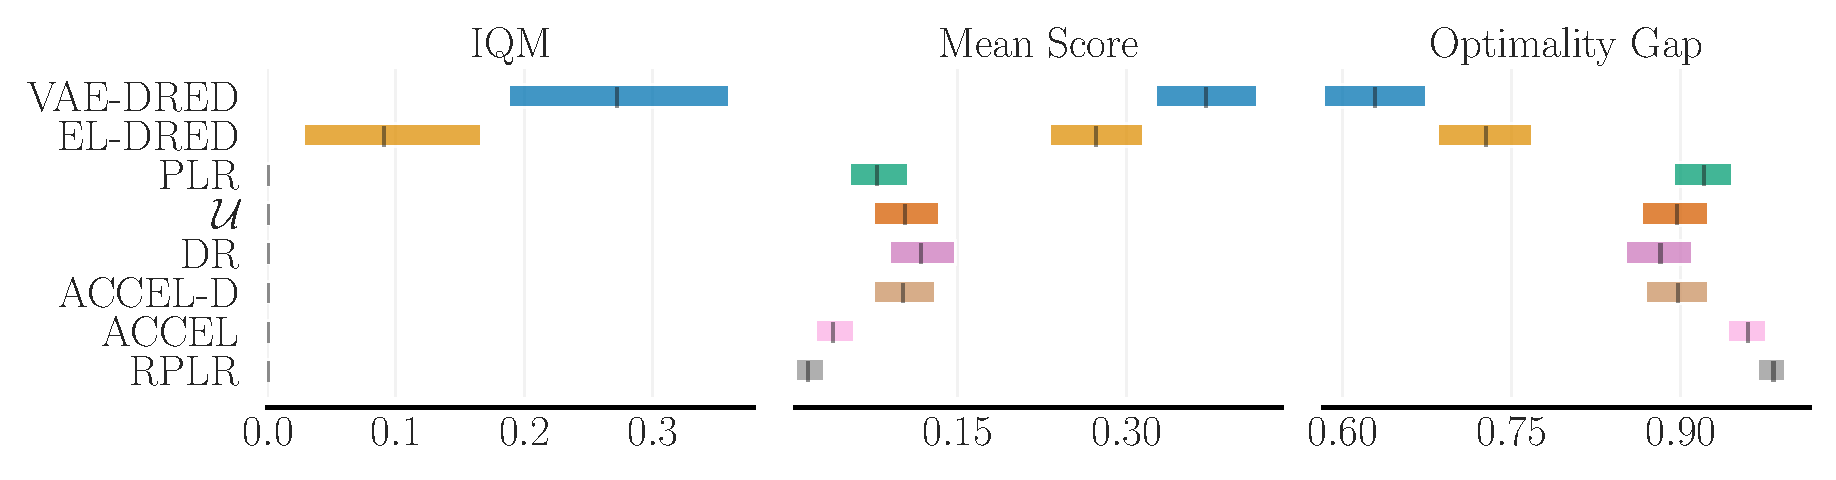
\includegraphics[width=1\linewidth]{content/minigrid_rliable/FULL-Hardcore-test_returns-all.pdf}
  \end{subfigure}%
    \begin{subfigure}[]{.2\linewidth}
    \centering
    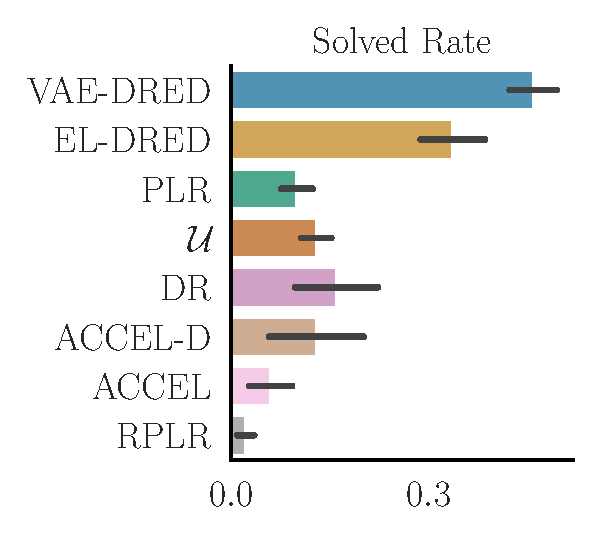
\includegraphics[width=1\linewidth]{content/solved_rates/solved_rate_Hardcoreall.pdf}
    \end{subfigure}%
\caption{Aggregate final performance and mean solved rate on 216 ``Hardcore'' levels, with a 45x45 layout size, making Hardcore layouts 9 times larger than $X_\text{train}$ layouts. Example layouts from each evaluation set are plotted on the left. The coloured boxes indicate a 99\% confidence interval and the black horizontal bars indicate standard error across 5 training seeds. We refer the reader to \Cref{app:cmdp_levelset} for additional details on our evaluation sets.}
\label{fig:zsg_hard_set_and_edge_cases}
% \vspace{-1.5em}
\end{figure}

\begin{table}[H]
\caption{Mean scores achieved in the Minigrid setting for each level evaluation dataset. We report the mean and standard deviation across 5 training runs, each corresponding to a different random seed. For each run the mean score is obtained by evaluating the final policy’s once in each level of the corresponding level dataset, and averaging. Bolded methods are not significantly different from the method with highest mean ($p<0.05$), unless all are, in which case none are bolded.}
\label{tb:minigrid_scores}
\vskip 0.15in
\begin{center}
\begin{small}
\begin{sc}
\tabcolsep=0.11cm
\begin{tabular}{lrrrrrrrr}
\toprule
      Level\\ datasets &                 VAE-DRED &                  EL-DRED &                      PLR &            $\mathcal{U}$ &              DR &         ACCEL-D &           ACCEL &            RPLR \\
\midrule
$X_{\mathrm{train}}$ & \textbf{0.92 $\pm$ 0.00} & \textbf{0.90 $\pm$ 0.03} & \textbf{0.92 $\pm$ 0.00} & \textbf{0.93 $\pm$ 0.01} & 0.37 $\pm$ 0.22 & 0.56 $\pm$ 0.11 & 0.27 $\pm$ 0.13 & 0.24 $\pm$ 0.07 \\
 $X_{\mathrm{test}}$ & \textbf{0.82 $\pm$ 0.02} & \textbf{0.77 $\pm$ 0.05} &          0.68 $\pm$ 0.03 &          0.67 $\pm$ 0.03 & 0.38 $\pm$ 0.22 & 0.49 $\pm$ 0.16 & 0.29 $\pm$ 0.14 & 0.24 $\pm$ 0.06 \\
              Edge C & \textbf{0.74 $\pm$ 0.05} & \textbf{0.67 $\pm$ 0.11} &          0.35 $\pm$ 0.11 &          0.32 $\pm$ 0.04 & 0.37 $\pm$ 0.21 & 0.34 $\pm$ 0.17 & 0.25 $\pm$ 0.14 & 0.17 $\pm$ 0.05 \\
            Hardcore & \textbf{0.37 $\pm$ 0.06} & \textbf{0.27 $\pm$ 0.07} &          0.08 $\pm$ 0.04 &          0.10 $\pm$ 0.04 & 0.12 $\pm$ 0.09 & 0.10 $\pm$ 0.11 & 0.04 $\pm$ 0.04 & 0.02 $\pm$ 0.02 \\
\bottomrule
\end{tabular}
\end{sc}
\end{small}
\end{center}
\vskip -0.1in
\end{table}

\begin{table}[H]
\caption{Solved rates achieved in the Minigrid setting for each level evaluation dataset. We report the mean and standard deviation across 5 training runs, each corresponding to a different random seed. For each run the solved rate is obtained by counting how many levels were solved (i.e. the agent reached the goal) after evaluating the final policy’s once in each level of the corresponding level dataset. Bolded methods are not significantly different from the method with highest mean ($p<0.05$), unless all are, in which case none are bolded.}
\label{tb:minigrid_solved_rate}
\vskip 0.15in
\begin{center}
\begin{small}
\begin{sc}
\tabcolsep=0.11cm
\begin{tabular}{lrrrrrrrr}
\toprule
      Level\\ datasets &                 VAE-DRED &                  EL-DRED &                      PLR &            $\mathcal{U}$ &              DR &         ACCEL-D &           ACCEL &            RPLR \\
\midrule
$X_{\mathrm{train}}$ & \textbf{1.00 $\pm$ 0.00} & \textbf{0.98 $\pm$ 0.03} & \textbf{1.00 $\pm$ 0.00} & \textbf{0.99 $\pm$ 0.00} & 0.48 $\pm$ 0.27 & 0.66 $\pm$ 0.15 & 0.34 $\pm$ 0.18 & 0.28 $\pm$ 0.09 \\
 $X_{\mathrm{test}}$ & \textbf{0.95 $\pm$ 0.01} & \textbf{0.89 $\pm$ 0.06} &          0.79 $\pm$ 0.03 &          0.77 $\pm$ 0.02 & 0.49 $\pm$ 0.26 & 0.57 $\pm$ 0.20 & 0.36 $\pm$ 0.19 & 0.29 $\pm$ 0.08 \\
              Edge C & \textbf{0.87 $\pm$ 0.06} & \textbf{0.80 $\pm$ 0.14} &          0.45 $\pm$ 0.12 &          0.40 $\pm$ 0.05 & 0.46 $\pm$ 0.25 & 0.41 $\pm$ 0.22 & 0.31 $\pm$ 0.19 & 0.19 $\pm$ 0.06 \\
            Hardcore & \textbf{0.46 $\pm$ 0.07} & \textbf{0.34 $\pm$ 0.10} &          0.10 $\pm$ 0.05 &          0.13 $\pm$ 0.05 & 0.16 $\pm$ 0.13 & 0.13 $\pm$ 0.14 & 0.06 $\pm$ 0.07 & 0.02 $\pm$ 0.03 \\
\bottomrule
\end{tabular}
\end{sc}
\end{small}
\end{center}
\vskip -0.1in
\end{table}

\begin{table}[H]
\caption{$\text{GenGap}$ and $\text{ShiftGap}$ at the end of training for each method tested. We report their mean and standard deviation across 5 training runs, each corresponding to a different random seed. Bolded methods are not significantly different from the method with lowest mean ($p<0.05$), unless all are, in which case none are bolded.}
\label{tb:minigrid_gen_metrics}
\vskip 0.15in
\begin{center}
\begin{small}
\begin{sc}
\tabcolsep=0.11cm
\begin{tabular}{lrrrrrrrr}
\toprule
           Metric &                  VAE-DRED &                   EL-DRED &                       PLR &            $\mathcal{U}$ &                        DR &         ACCEL-D &                     ACCEL &                      RPLR \\
\midrule
  $\text{GenGap}$ &           0.09 $\pm$ 0.01 &           0.14 $\pm$ 0.03 &           0.24 $\pm$ 0.03 &          0.25 $\pm$ 0.02 & \textbf{-0.00 $\pm$ 0.01} & 0.08 $\pm$ 0.05 & \textbf{-0.02 $\pm$ 0.02} & \textbf{-0.01 $\pm$ 0.01} \\
$\text{ShiftGap}$ & \textbf{0.00 $\pm$ 0.04} & \textbf{-0.08 $\pm$ 0.11} & \textbf{-0.07 $\pm$ 0.14} & n/a (0) &  \textbf{0.16 $\pm$ 0.20} & 0.25 $\pm$ 0.16 &           0.66 $\pm$ 0.17 &  \textbf{0.18 $\pm$ 0.45} \\
     $\text{JSD}$ &           \textbf{0.11 $\pm$ 0.01} &           0.16 $\pm$ 0.02 &           0.29 $\pm$ 0.05 & n/a (0) &           0.42 $\pm$ 0.00 & 0.29 $\pm$ 0.03 &           0.38 $\pm$ 0.06 &           0.46 $\pm$ 0.04 \\
\bottomrule
\end{tabular}
\end{sc}
\end{small}
\end{center}
\vskip -0.1in
\end{table}

% \subsection{Training levels generated by each method}

\section{CMDP specification and generation}\label{app:cmdp_levelset}

%\footnote{A link to the open source repository will be included in the de-anonymised version}
In Minigrid \cite{gym_minigrid}, the agent receives as an observation a partial view of its surroundings (in our experiments it is set to two tiles to each side of the agent and four tiles in front) and a one-hot vector representing the agent's heading. The action space consists of 7 discrete actions but, in our setting, only the actions moving the agent forward and rotating it to the left or right have an effect. The episode starts with the agent at its start tile and facing its starting orientiation. The episode terminates successfully when the agent reaches the goal tile. It receives a reward between 0 and 1 based on the number of timesteps it took to get there. The episode will terminate without a reward if the agent steps on a lava tile, or when the maximum number of timesteps is reached.

Levels are parameterised as 2D grids representing the overall layout, with each tile type represented by an unique ID. Tiles can be classified as navigable (for example, moss or empty tiles) or non-navigable (for example, walls and lava, as stepping into lava terminates the episode). To be valid, a level must possess exactly one goal and start tile, and to be solvable there must exist a navigable path between the start and the goal location. We provide the color palette of tiles used in \Cref{fig:color_palette}.

We provide example levels of the CMDP in \Cref{fig:layouts_dataset}. The CMDP level space corresponds to the subset of solvable levels in which moss and lava node placement is respectively positively and negatively correlated with their shortest path distance to the goal.\footnote{To measure the shortest path distance to goal of a non-navigable node, we first find the navigable node that is closest from it and measure its shortest path distance to the goal. We then add to it the number of tile separating this navigable node to the non-navigable node of interest. If there are multiple equally close navigable nodes, we select the navigable node with the smallest shortest path distance to the goal.} Under partial observability, the optimal policy for this CMDP would leverage moss and lava locations as contextual cues, seeking regions with high moss density and avoiding regions with high lava density. 

\begin{figure}[!htb]

% preliminary
\sbox\twosubbox{%
  \resizebox{\dimexpr.7\textwidth-1em}{!}{%
    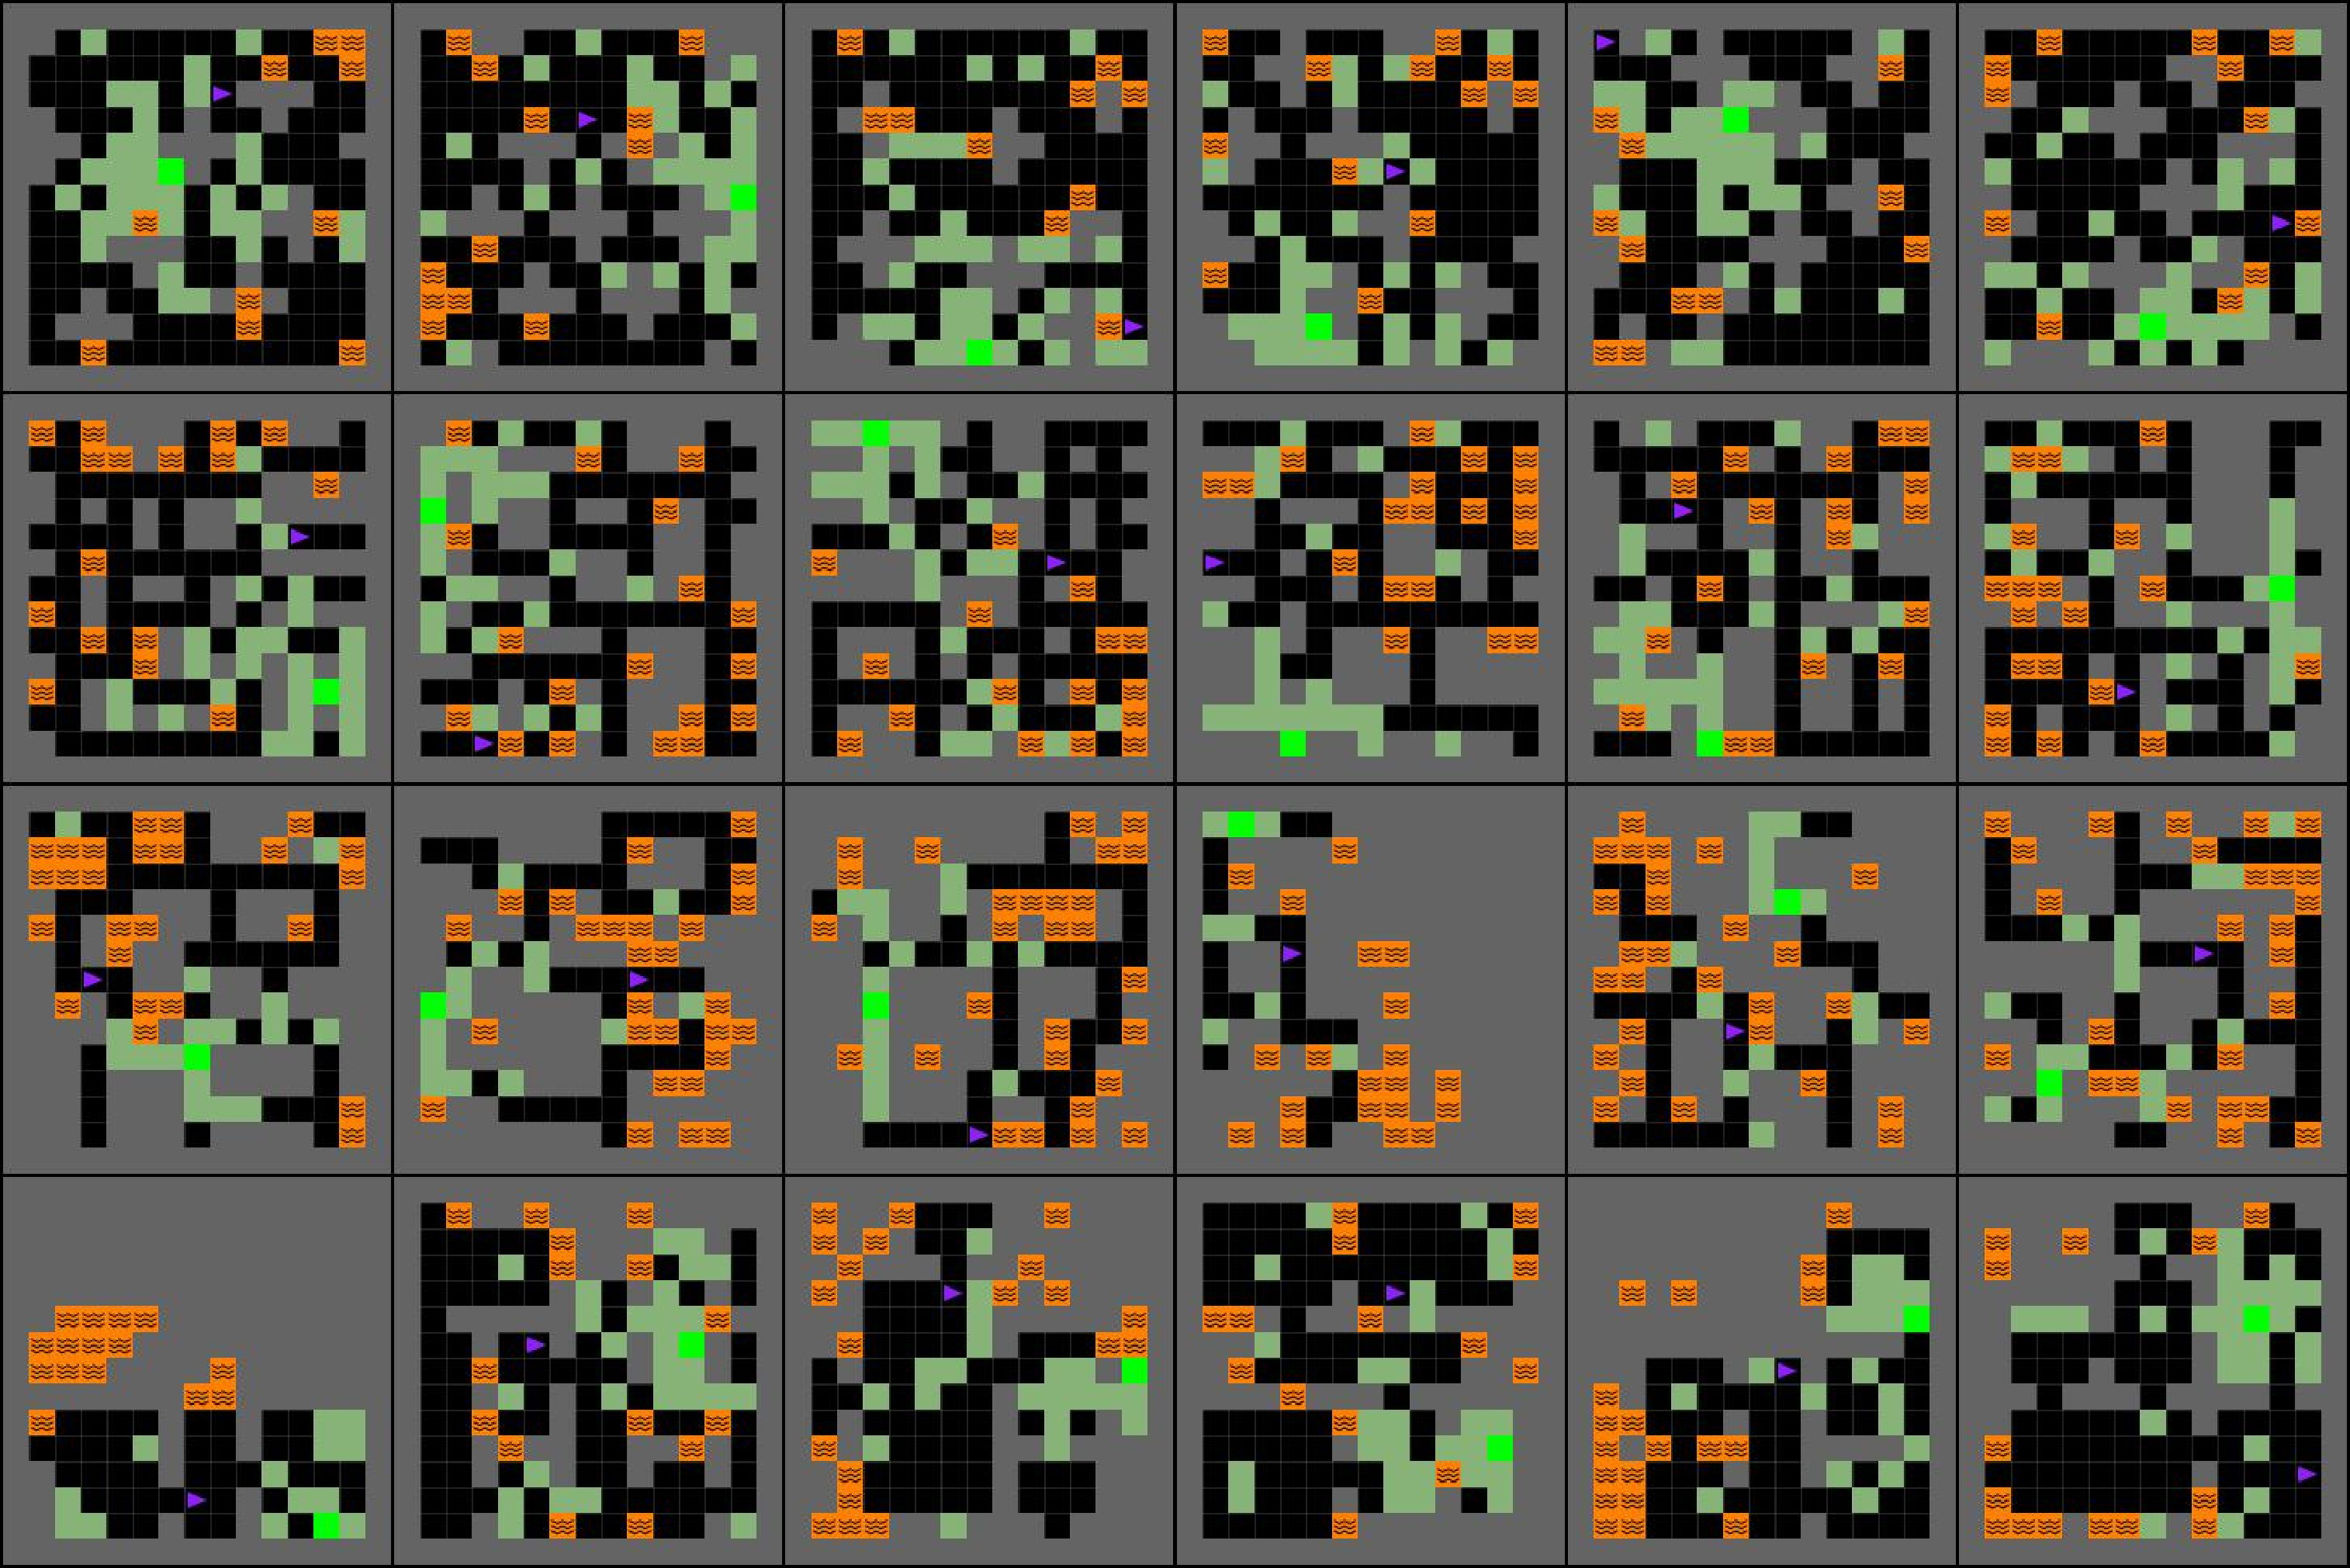
\includegraphics[height=3cm]{app_content/layouts/cave_escape_dataset.pdf}%
    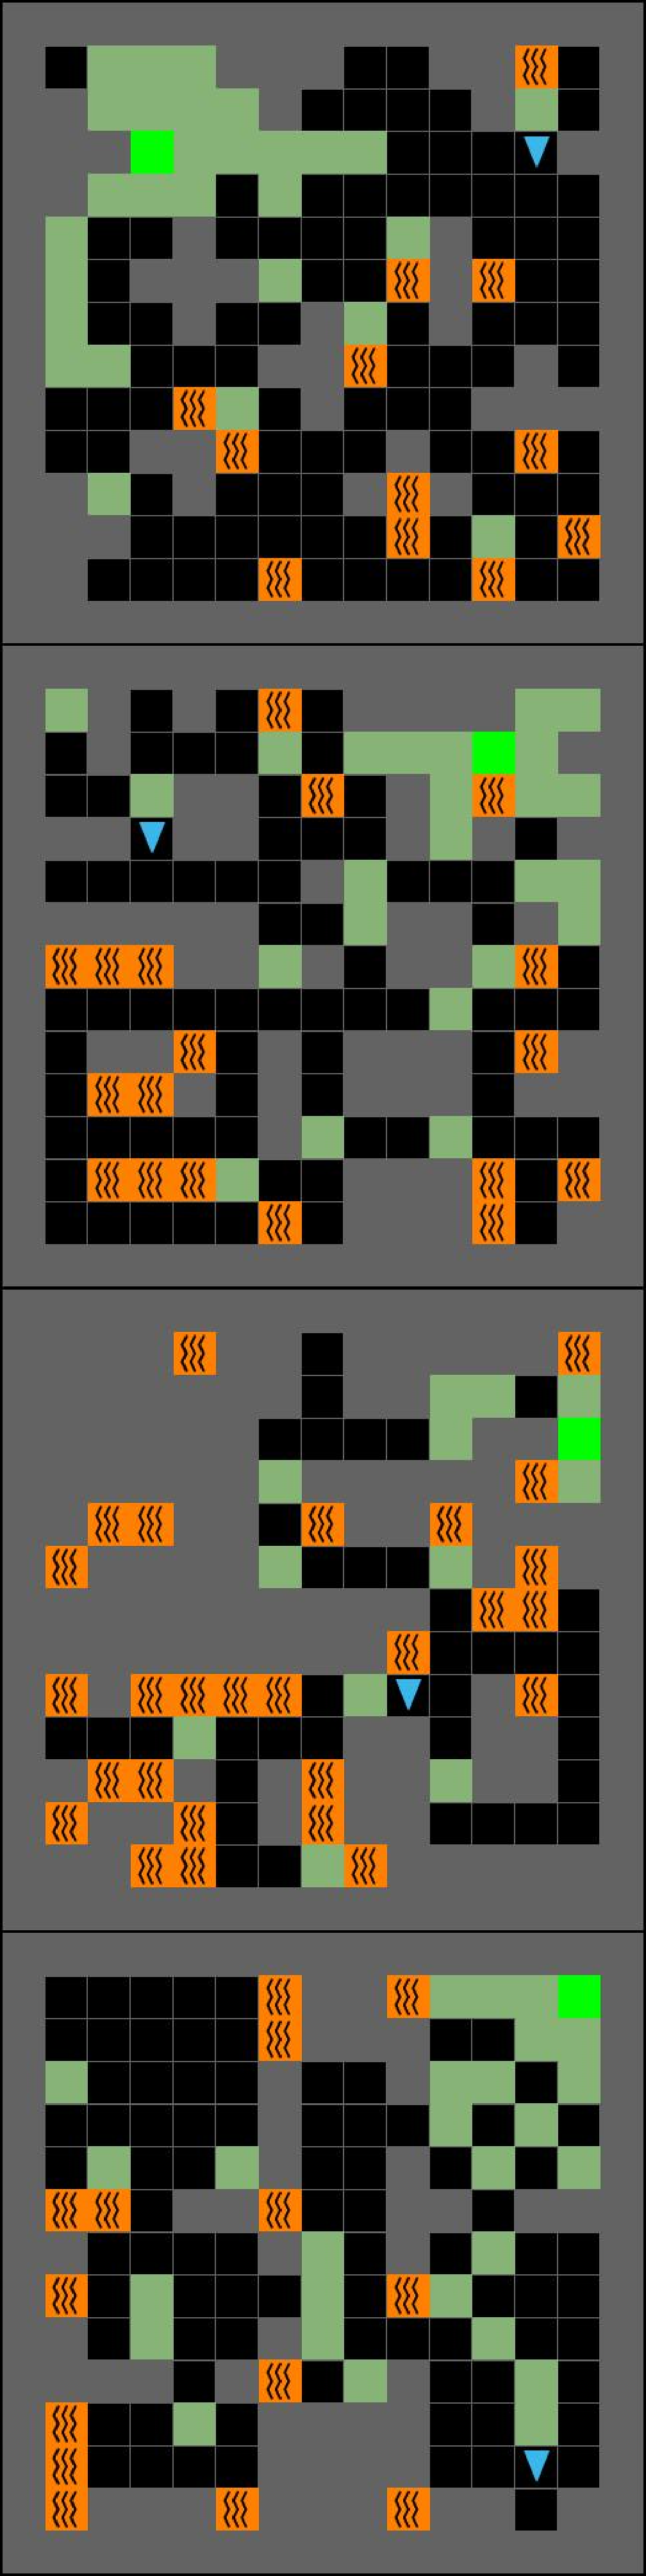
\includegraphics[height=3cm]{app_content/layouts/cave_escape_16k_4ts_id_rotated.pdf}%
  }%
}
\setlength{\twosubht}{\ht\twosubbox}

% typeset

\centering

\subcaptionbox{Example training levels from $X_\text{train}$\label{f}}{%
  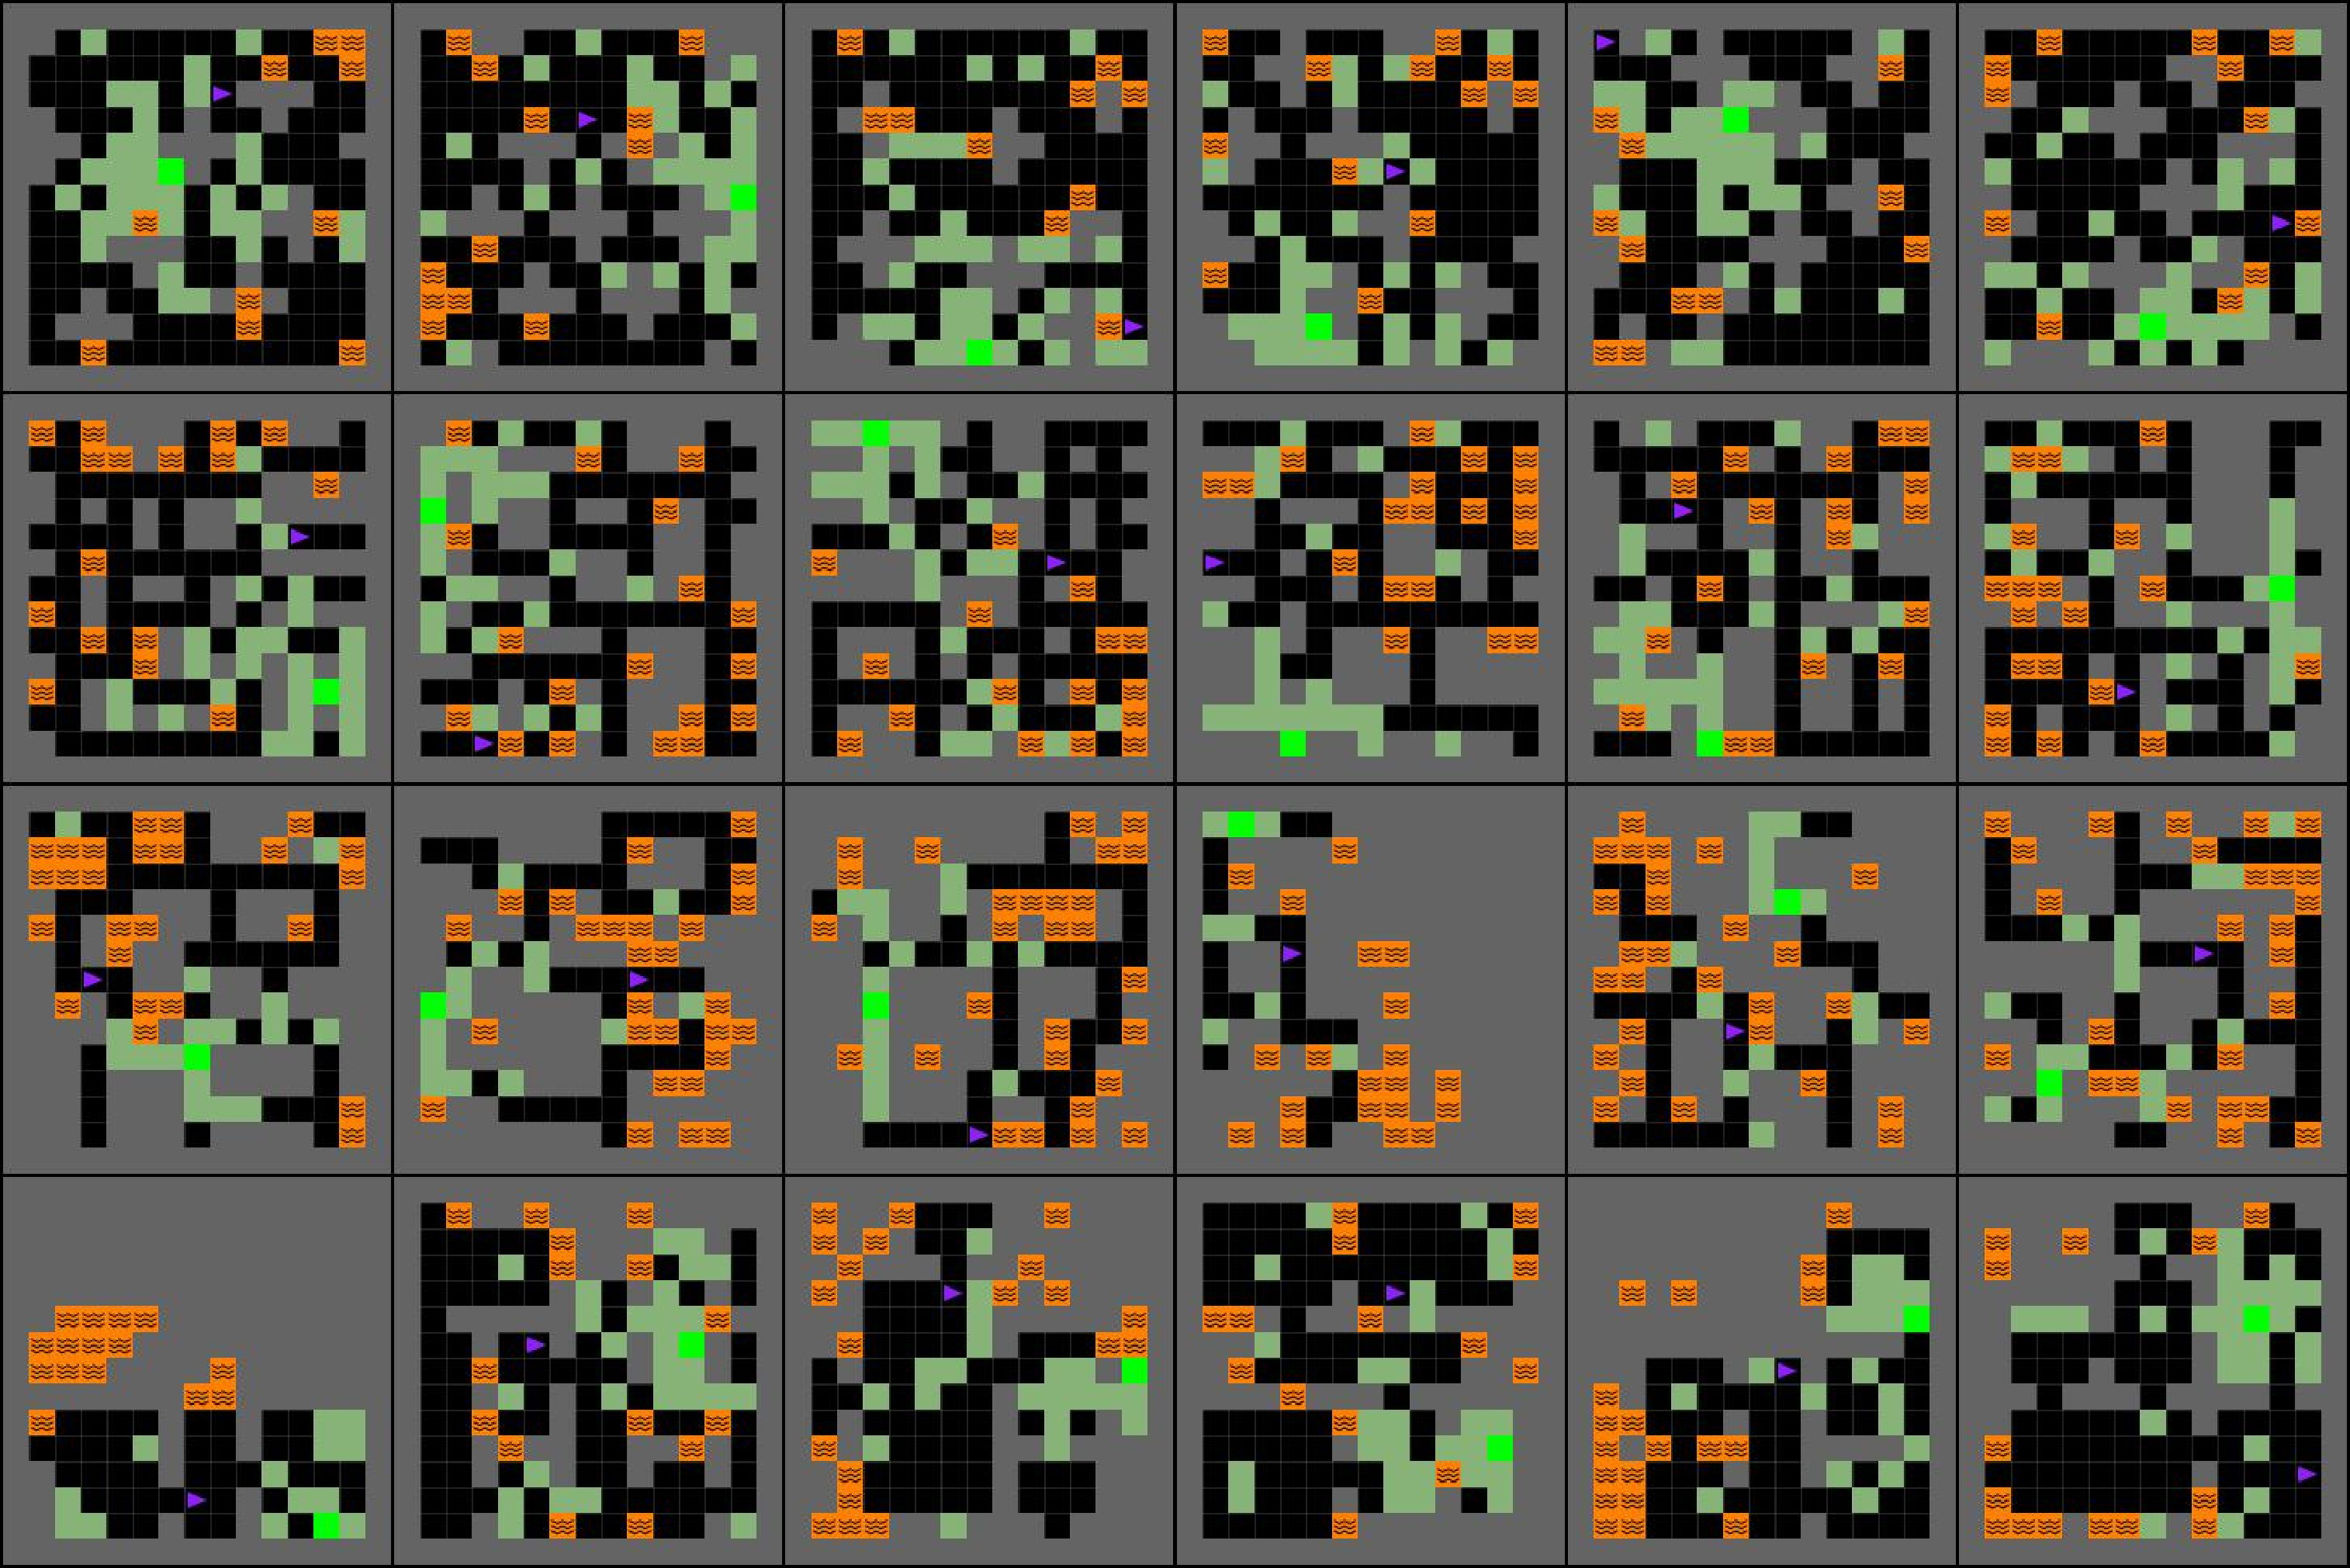
\includegraphics[height=\twosubht]{app_content/layouts/cave_escape_dataset.pdf}%
}\quad
\subcaptionbox{Held-out levels\label{s1}}{%
  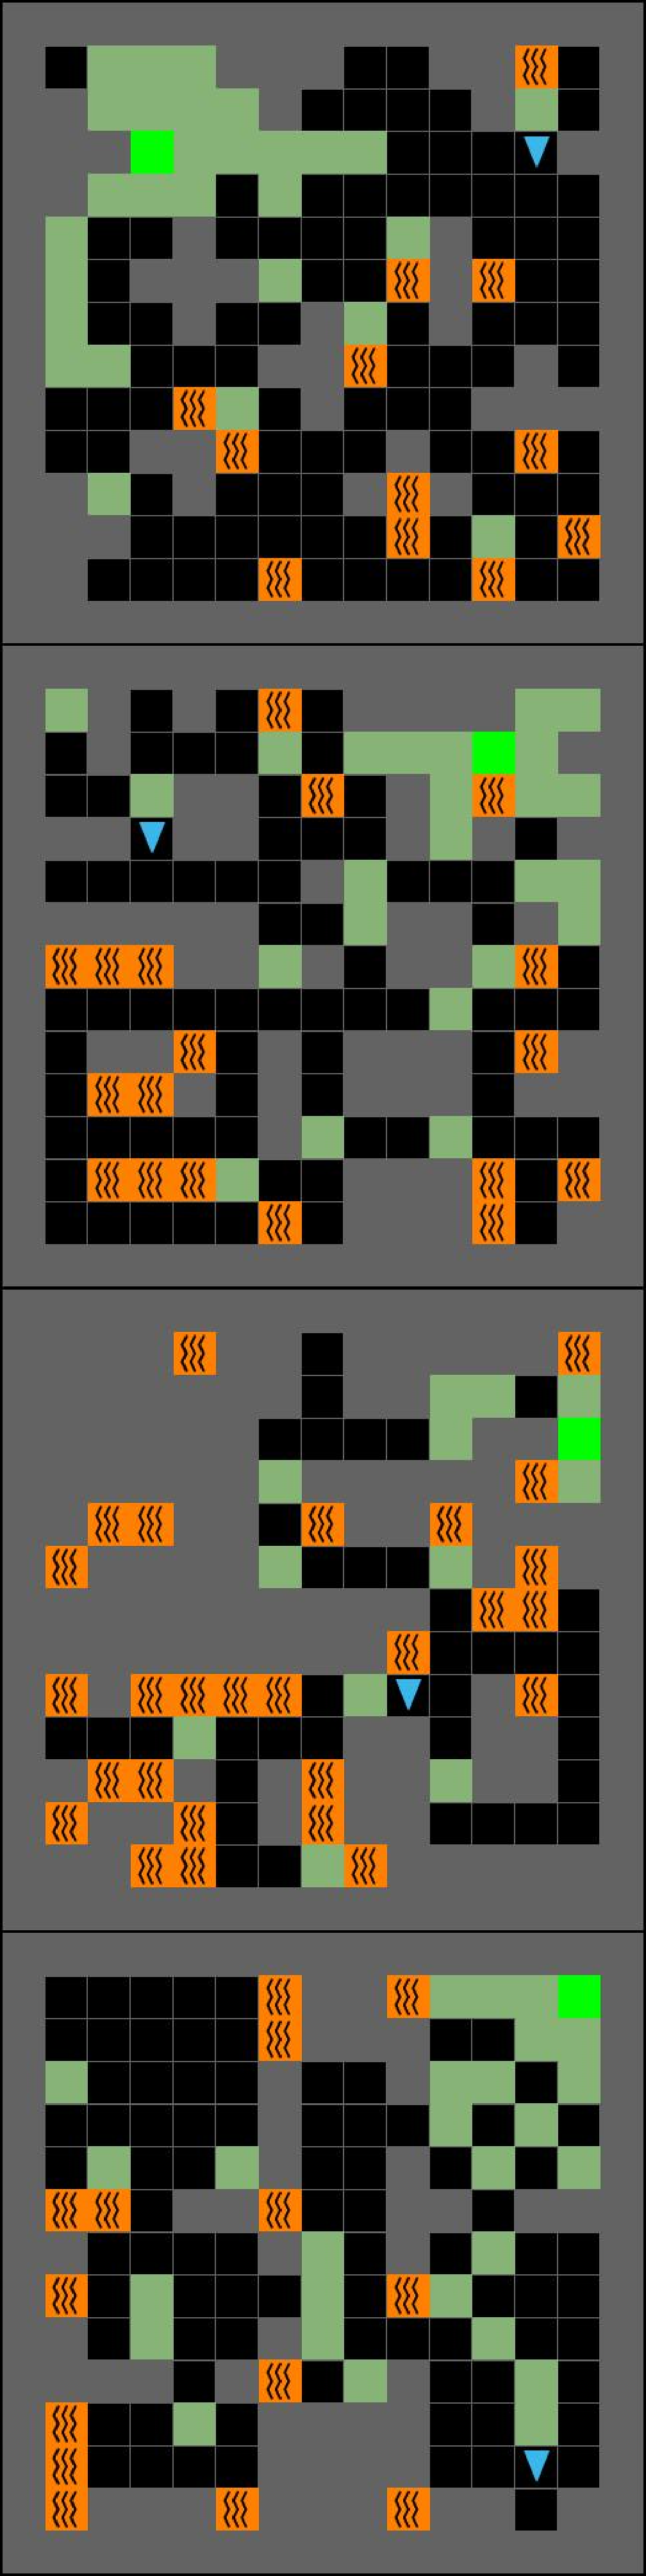
\includegraphics[height=\twosubht]{app_content/layouts/cave_escape_16k_4ts_id_rotated.pdf}%
}

\caption{Sample levels from $X_\text{train}$ and from held-out test set $X_\text{test}$. Wall tiles are rendered in gray, empty tiles in black, moss tiles in green and the goal tile in lime green. The agent is rendered as a blue or purple triangle, and is depicted at its start location. Each row corresponds to levels generated with a specific wave function collapse base pattern. Four different base patterns are used to generate $X_\text{train}$ and $X_\text{test}$ layouts. As in Procgen games, we find that the PPO agent exhibits a significant $\text{GenGap}$ on held-out levels when being restricted to train on 200-500 levels. We therefore have $X_\text{train}$ contain 512 levels and we have $X_\text{test}$ contain 2048 levels for more accurate agent evaluation.}\label{fig:layouts_dataset}

\end{figure}

\begin{figure}[!htb]

% preliminary
\sbox\twosubbox{%
  \resizebox{\dimexpr.9\textwidth-1em}{!}{%
    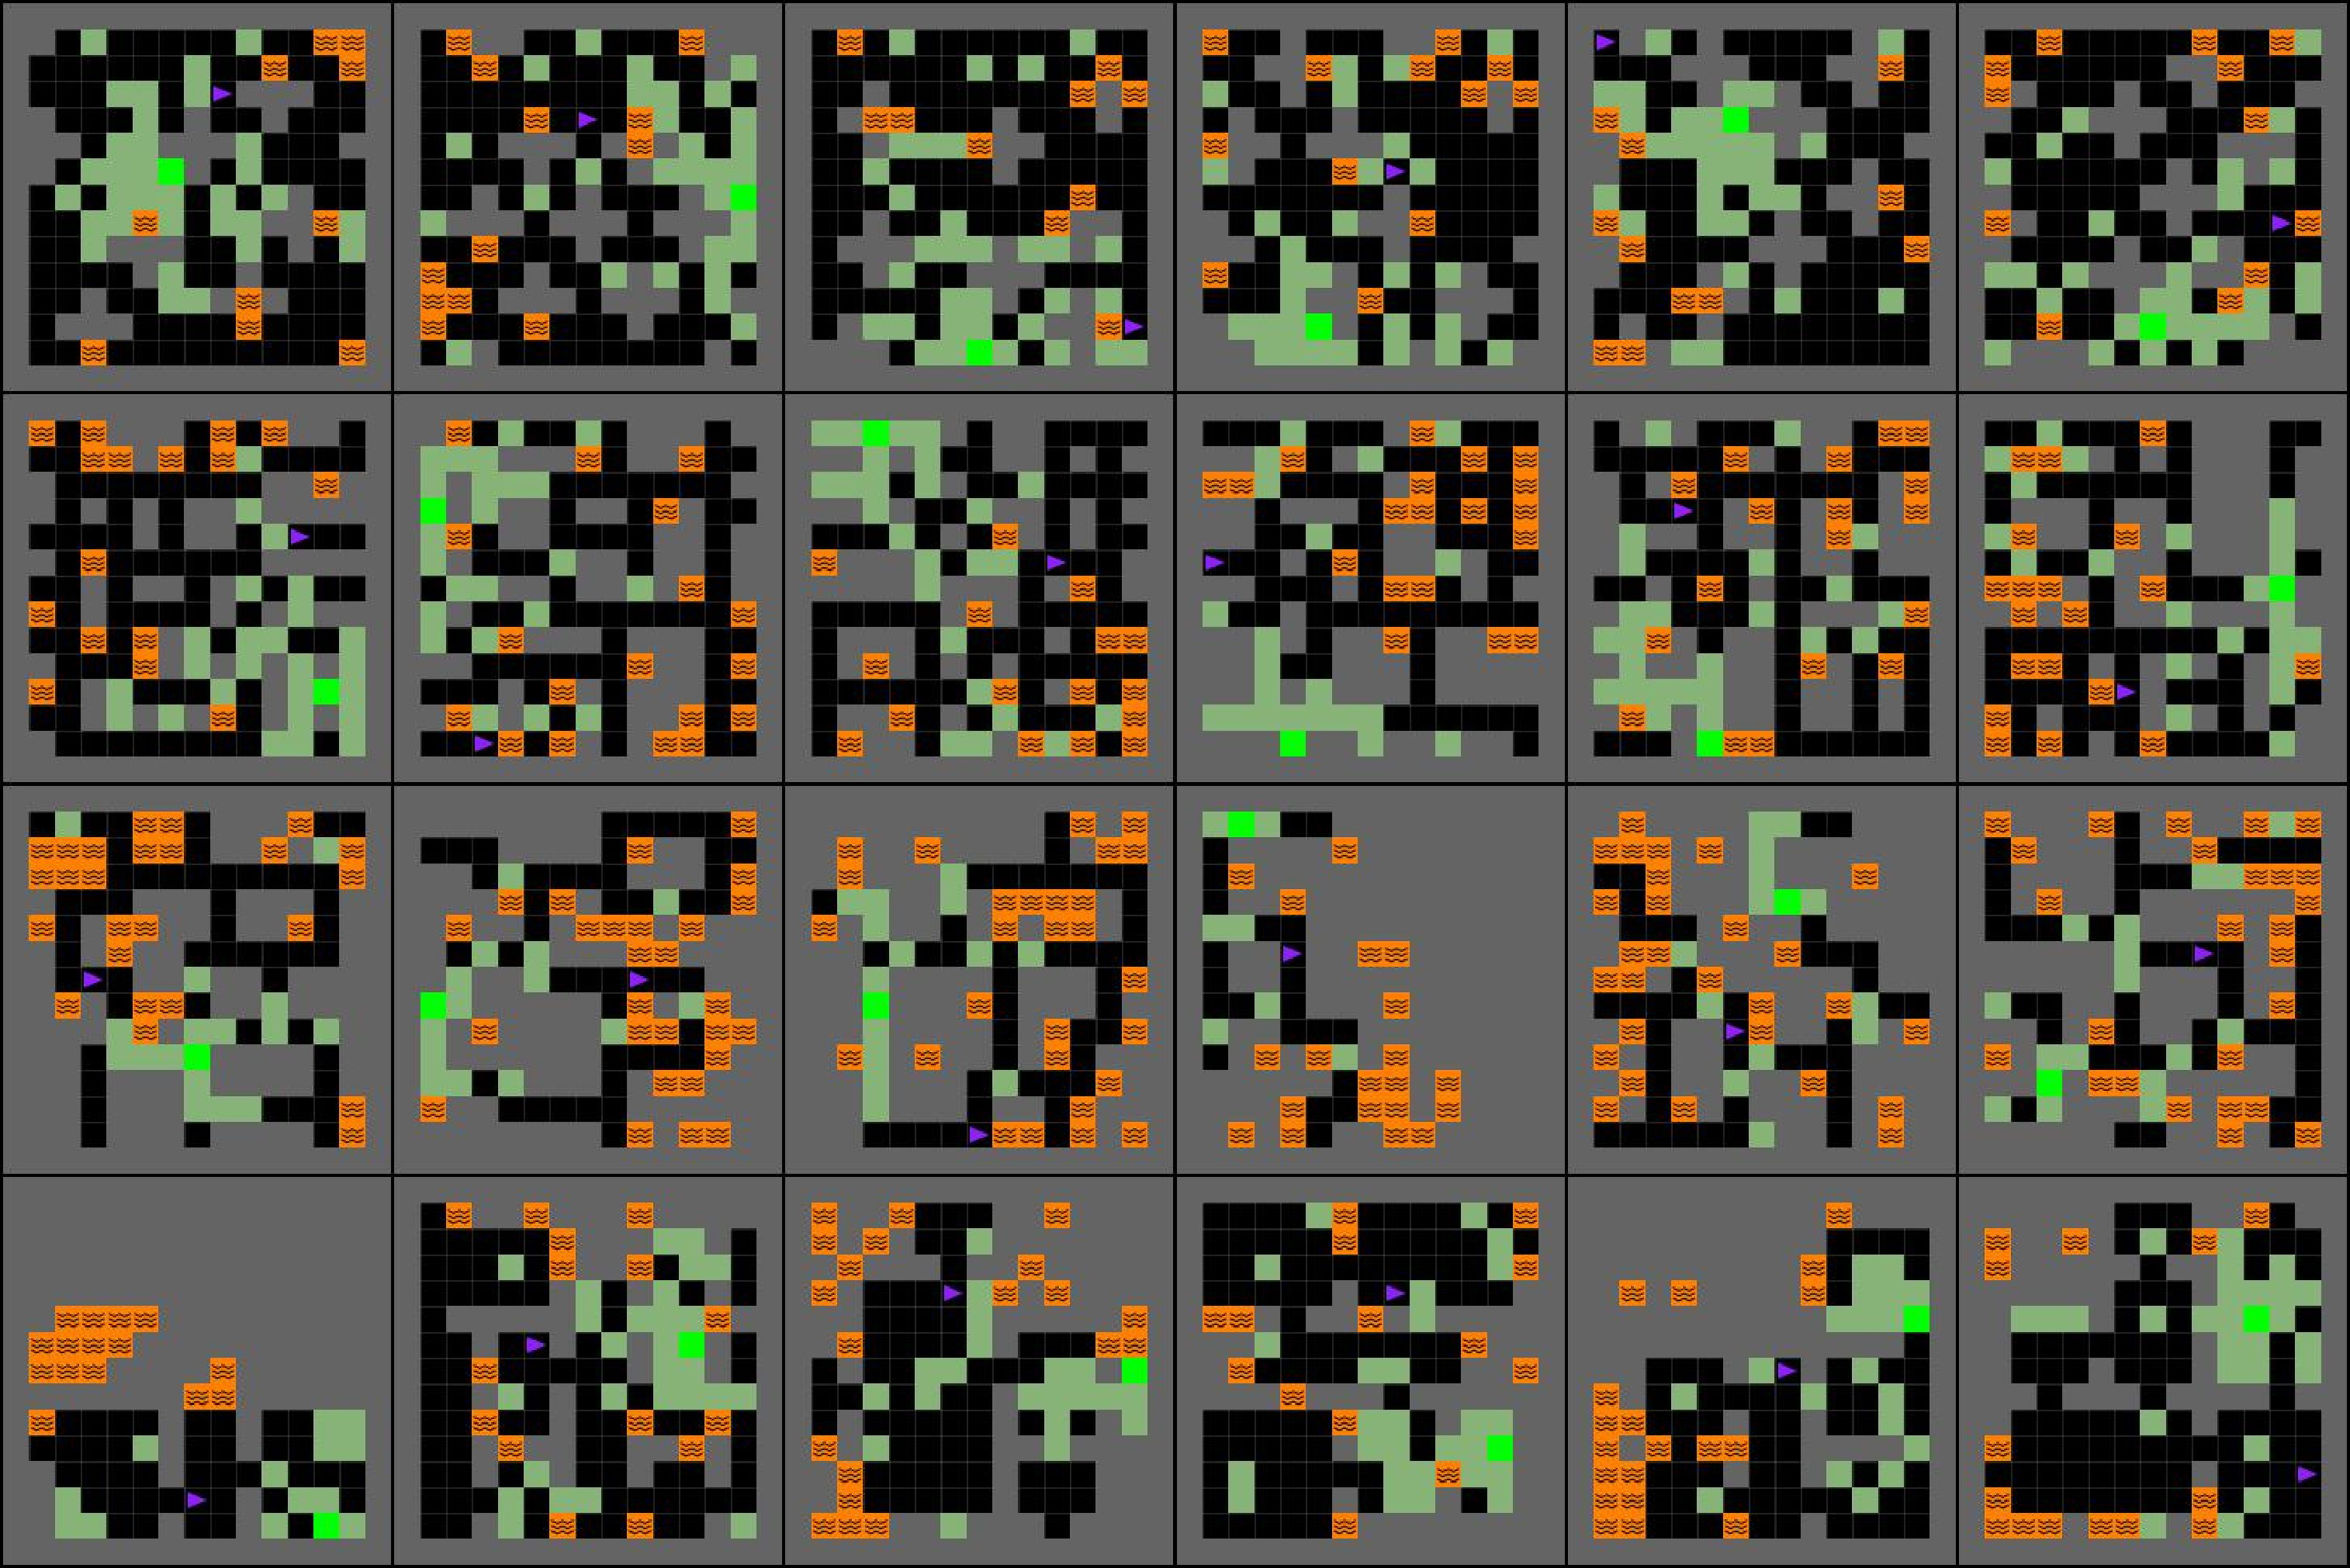
\includegraphics[height=3cm]{app_content/layouts/cave_escape_dataset.pdf}%
    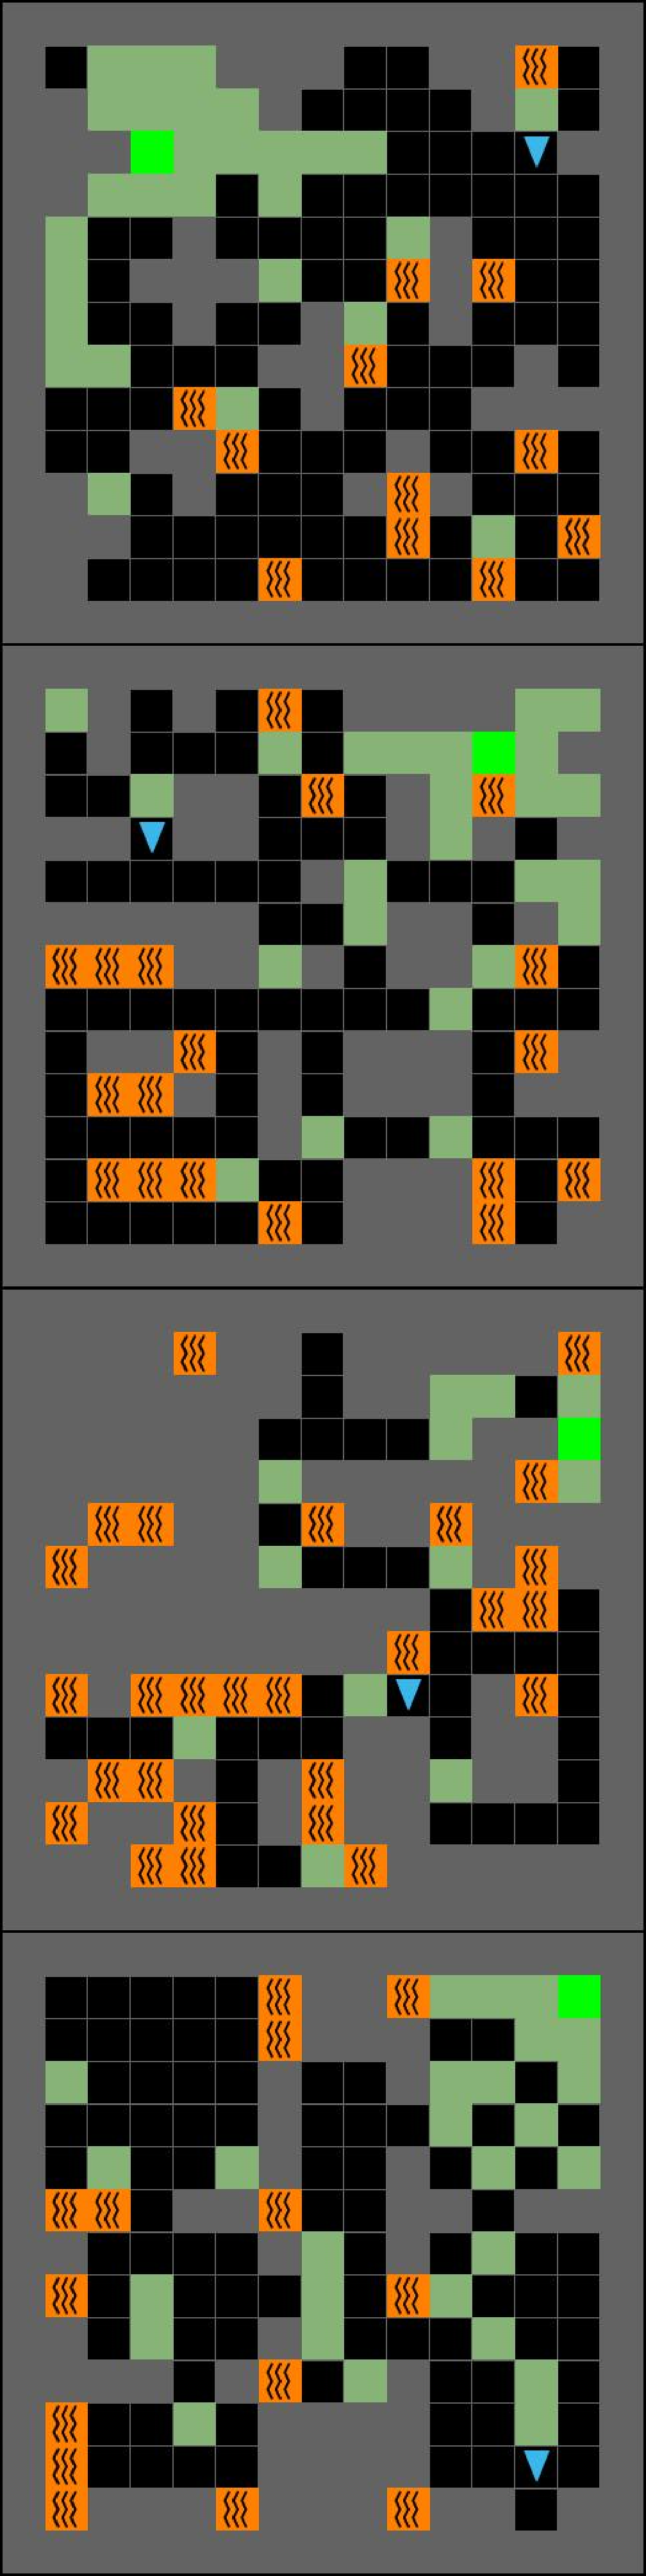
\includegraphics[height=3cm]{app_content/layouts/cave_escape_16k_4ts_id_rotated.pdf}%
  }%
}
\setlength{\twosubht}{\ht\twosubbox}

% typeset

\centering

\subcaptionbox{Example levels from the first set of edge cases}{%
  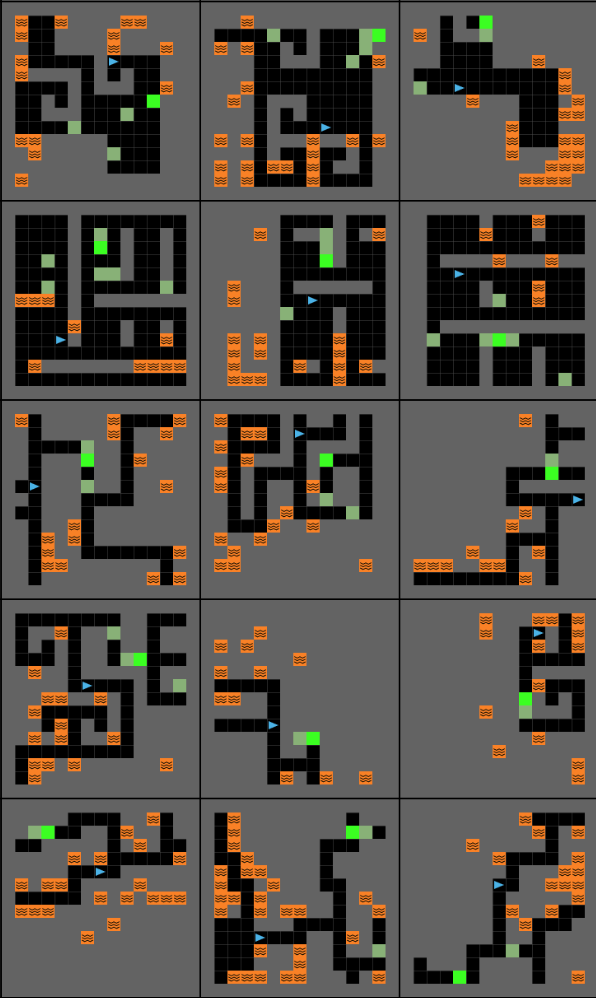
\includegraphics[height=\twosubht]{app_content/layouts/little_moss_layouts.png}%
}\quad
\subcaptionbox{Example levels from the second set of edge cases\label{s2}}{%
  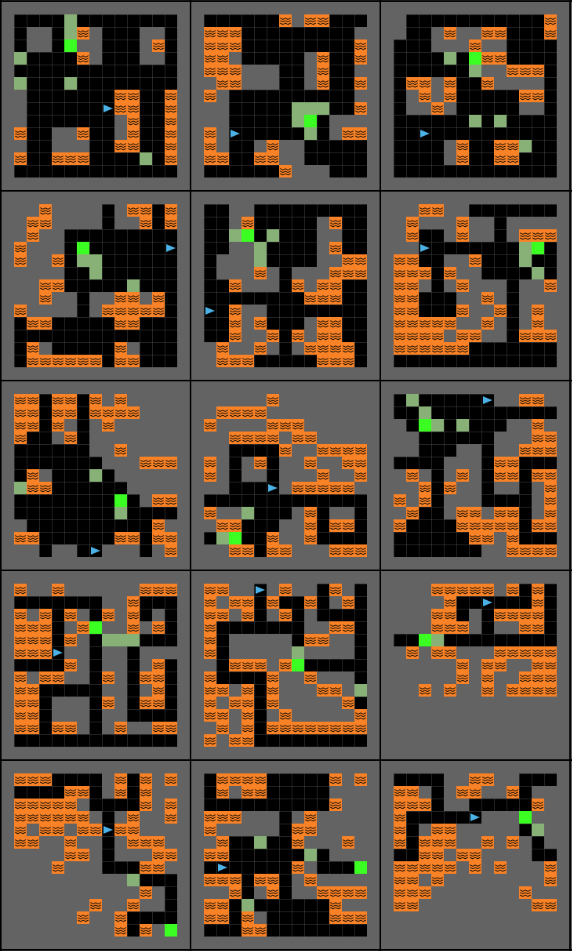
\includegraphics[height=\twosubht]{app_content/layouts/lots_of_lava_layouts.png}%
}

\caption{We generate 2 separate sets of edge cases, using 14 different base patterns not used to generate $X_\text{train}$. The moss density of the first set (a) is 2 to 5 times as small as levels found within $X_\text{train}$, making finding the goal using CMDP contextual cues more challenging. (b) is the same as (a) but with a lava tile density 2 to 5 times higher than $X_\text{train}$ levels, which makes avoiding lava more challenging. Both sets contain the same number of levels (224), and they are combined when evaluating the agent on edge cases.}\label{fig:layout_edge_cases}

\end{figure}

\subsection{Generating highly structured levels}

We use the wave function collapse (WFC) procedural generation algorithm \citep{WFC} to obtain highly structured but still diverse gridworld layouts. WFC gradually collapses a superposition of all possible level parameters into a layout respecting the constraints defined by an input pattern. By doing so, it is possible to generate a vast number of tasks from a small number of starting patterns. Given a suitable base pattern, WFC provides a high degree of structure and complexity in generated layouts, and it guarantees that both task structure and diversity scale with the gridworld dimensions. Our implementation supports generating layouts from 22 %TODO: check
different base patterns, and supports the specification of custom user-defined patterns. 

After generating a layout using WFC, we convert the navigable nodes of a layout into a graph, choose its largest connected component as the layout and convert any unreachable nodes to non-navigable nodes. We place the goal location at random and place the start at a node located at the median geodesic distance from the goal in the navigation graph. By doing so we ensure that the complexity of generated layouts is relatively consistent given a specific grid size and base pattern. Finally, we sample tiles according to parameterisable distributions defined over the navigable and non-navigable node sets. 

In our experiments, the tile set consists of the $\{$ moss, empty, start, goal $\}$ tiles as the navigable set and the $\{$ wall, lava$\}$ tiles as the non-navigable set. We parameterise tile distributions such that moss tiles are more likely to be sampled on navigable nodes close to the goal, while lava tiles are more likely on non-navigable nodes far away from the goal.

\subsection{Controlling level complexity}

We provide two options to vary the complexity of the level distribution. The first is to change the layout size. Due to partial observability this significantly increases their complexity, and makes levels from the ``Hardcore'' set depicted in \Cref{fig:zsg_hard} challenging to solve for Human players. The second option is to change the sampling probability of moss and lava tiles. Reducing the fraction of moss to navigable tiles diminishes their usefulness as context cues. On the other hand, increasing the density of lava tiles increases the risk associated with selecting the wrong action during play. In our experiments we assess the agent's performance on edge-cases by defining level sets with a larger layout size (\Cref{fig:zsg_hard}), or with different moss and lava tile distributions (\Cref{fig:layout_edge_cases}).  

\section{Implementation details}\label{app:imp_details}

\subsection{Procgen}\label{app:procgen}
The Procgen Benchmark is a set of 16 diverse PCG environments that echoes the gameplay variety seen in the ALE benchmark \cite{ALE}. The game levels, determined by a random seed, can differ in visual design, navigational structure, and the starting locations of entities. All Procgen environments use a common discrete 15-dimensional action space and generate $64 \times 64 \times 3$ RGB observations. A detailed description of each of the 16 environments is provided in \citet{procgen}. RL algorithms such as PPO reveal significant differences between test and training performance in all games, making Procgen a valuable tool for evaluating generalisation performance. 

We conduct our experiment on the easy setting of Procgen, which employs 200 training levels and a budget of 25M training steps, and evaluate the agent's ZSG performance on the full range of levels, excluding the training levels.

We employ the same ResNet policy architecture and PPO hyperparameters (identical for all games) as \cite{procgen}, which we reference in \Cref{table:hyperparams}. To compute $\mut{L}{b}$ and the scoring strategy for $(S^\text{MI})$ in our experiments, we model $p_\vtheta(\lvl|b(o_t))$ as a linear classifier predicting the level identity from the output of the last shared network layer between the actor and critic. $p_\vtheta$ is trained using trajectory rollouts collected by sampling uniformly from $L$. We ensure the training processes of the agent and the classifier remain independent from one-another by employing a separate optimiser, and by stopping the gradients from propagating through the agent's network.

\subsection{Minigrid RL agent} \label{app:impl_minigrid}

We use the recurrent PPO agent and hyperparameters employed in \cite{ACCEL} for all our experiments. The actor and critic share their initial layers. The first initial layer consists of a convolutional layer with 16 output channels and kernel size 3 processes the agent's view and a fully connected layer that processes its directional information. Their output is concatenated and fed to an LSTM layer with hidden size 256. The actor and critic heads each consist of two fully connected layers of size 32, the actor outputs a categorical distribution over action probabilities while the critic outputs a scalar. Weights are optimised using Adam and we employ the same hyperparameters in all experiments, reported in \Cref{table:hyperparams}. Trajectories are collected via 36 worker threads, with each experiment conducted using a single GPU and 10 CPUs.

Following \cite{ACCEL}, DR and RPLR use domain randomisation as their standard level generation process, in which the start and goal locations, alongside a random number between 0 and 60 moss, wall or lava tiles are randomly placed. The level editing process of ACCEL and EL-DRED remains unchanged from \cite{ACCEL}, consisting of five steps. The first three steps may change a randomly selected tile to any of its counterparts, whereas the last two are reserved to replacing the start and goal locations if they had been removed in prior steps.

We train three different seeds for each baseline. We use the hyperparameters reported in \cite{ACCEL} for the DR, RPLR and ACCEL methods and the hyperparameters reported in \cite{PLR} for PLR, as an extensive hyperparameter search was conducted in a similarly sized Minigrid environment for each method. VAE-DRED employs the same hyperparameters as PLR for its level buffer, with some additional secondary sampling strategy hyperparameters introduced by VAE-DRED. We did not perform an hyperparameter search for VAE-DRED as we found that the initial values worked adequately. We report all hyperparameters in \Cref{table:hyperparams}.

\subsection{VAE architecture and pre-training procedure}\label{app:vae_imp}

We employ the $\beta-$VAE formulation proposed in \cite{betaVAE}, and we parametrise the encoder as a Graph Convolutional Network (GCN), a generalisation of the Convolutional Neural Network (CNN) \citep{CNNimagenet} to non Euclidian spaces. Our choice of a GCN architecture is not motivated by a desire of maximising the VAE's performance (in fact we expect a CNN or MLP encoder to work just as well in Minigrid). It is instead intended as a proof of concept for an architecture that could transfer to more complex simulators. Since the level parameter space $\sX$ is simulator-specific, employing a graph as an input modality for our encoder makes our model architecture easier to transfer to different simulators and domains. Using a GCN, some of the inductive biases that would be internal in a traditional architecture can be defined through an external wrapper that encodes the environment parameter $\vx$ into the graph $\mathcal{G}_\vx$. 

In Minigrid, we represent the gridworld levels as a grid graphs, each cell being an individual node. This effectively makes the GCN equivalent to a traditional CNN in this scenario. However a GCN provides ways of providing additional domain specific biases that a CNN lacks. For example, a domain expert with the notion that goal, lava and moss tiles are somehow correlated can add edges between these tiles in the graph.

We select the GIN architecture \citep{GIN} for the GCN, which we connect to an MLP network that outputs latent distribution parameters $(\vmu_\vz, \vsigma_\vz)$. The decoder is a fully connected network with three heads. The \textit{layout} head outputs the parameters of categorical distributions for each grid cell, predicting the tile identity between [Empty, Moss, Lava, Wall]. The \textit{start} and \textit{goal} heads output the parameters of categorical distributions predicting the identity of the start and goal locations across grid cells, ensuring a single goal or start node get sampled in any given level.

We pre-train the VAE for 200 epochs on $X_\text{train}$, using cross-validation for hyperparameter tuning, each run taking about 25 minutes on a GPU-equipped laptop. During training, we formulate the reconstruction loss as a weighted sum of the cross-entropy loss for each head.\footnote{To compute the cross-entropy loss of the layout head, we replace the start and goal nodes in the reconstruction targets by a uniform distribution across \{moss, empty\}.}%TODO: footnote on several pages, fix
At deployment, we guarantee \textit{valid} layouts  get generated (i.e. layouts containing a unique start and goal location, but not necessarily solvable) by generating level parameters sequentially. We first sample the layout, then we sample the start location, masking any non-navigable tile generated in the last step. We then add the start tile to our mask before sampling the goal location. In this way, we guarantee valid start and goal locations that will not override one-another. Note that our generative model may still generate \textit{unsolvable} layouts, which do not have a passable path between start and goal locations, and therefore it must have learnt to generate solvable layouts in order to be useful. 

We do not explicitly encourage the VAE to generate solvable levels, but we find that models with high ELBO (\Cref{eq:ELBO}) on the validation set tend to also have a high generated layout solvability rate. Layouts reconstructed from $X_\text{train}$ have over 80\% solvability rate, while layouts generated via latent space interpolations have over 70\% solvability rate. In practice, maximising the ELBO results in generated layouts sharing contextual semantics with $X_\text{train}$ levels. This can be observed qualitatively in the VAE-generated layouts included in \Cref{fig:interpolated_levels}, and quantitatively in \Cref{fig:gen_gaps,fig:buffermetrics}, where we report that contextually important semantics are transferred to the agent's training distribution.

To tune the VAE we conduct a random sweep over architectural parameters (number of layers, layer sizes), the $\beta$ coefficient, individual decoder head reconstruction coefficients and the learning rate over a total budget of 100 runs. We select the configuration achieving the highest ELBO on the validation set. These hyperparameters are reported in %Each run takes 20 minutes, which means that our sweeping procedure takes less time to complete than a single seed of our Minigrid experiment. 
\Cref{table:hyperparams_vae}.

\begin{figure}[!htb]

% preliminary
\sbox\twosubbox{%
  \resizebox{\dimexpr.9\textwidth-1em}{!}{%
    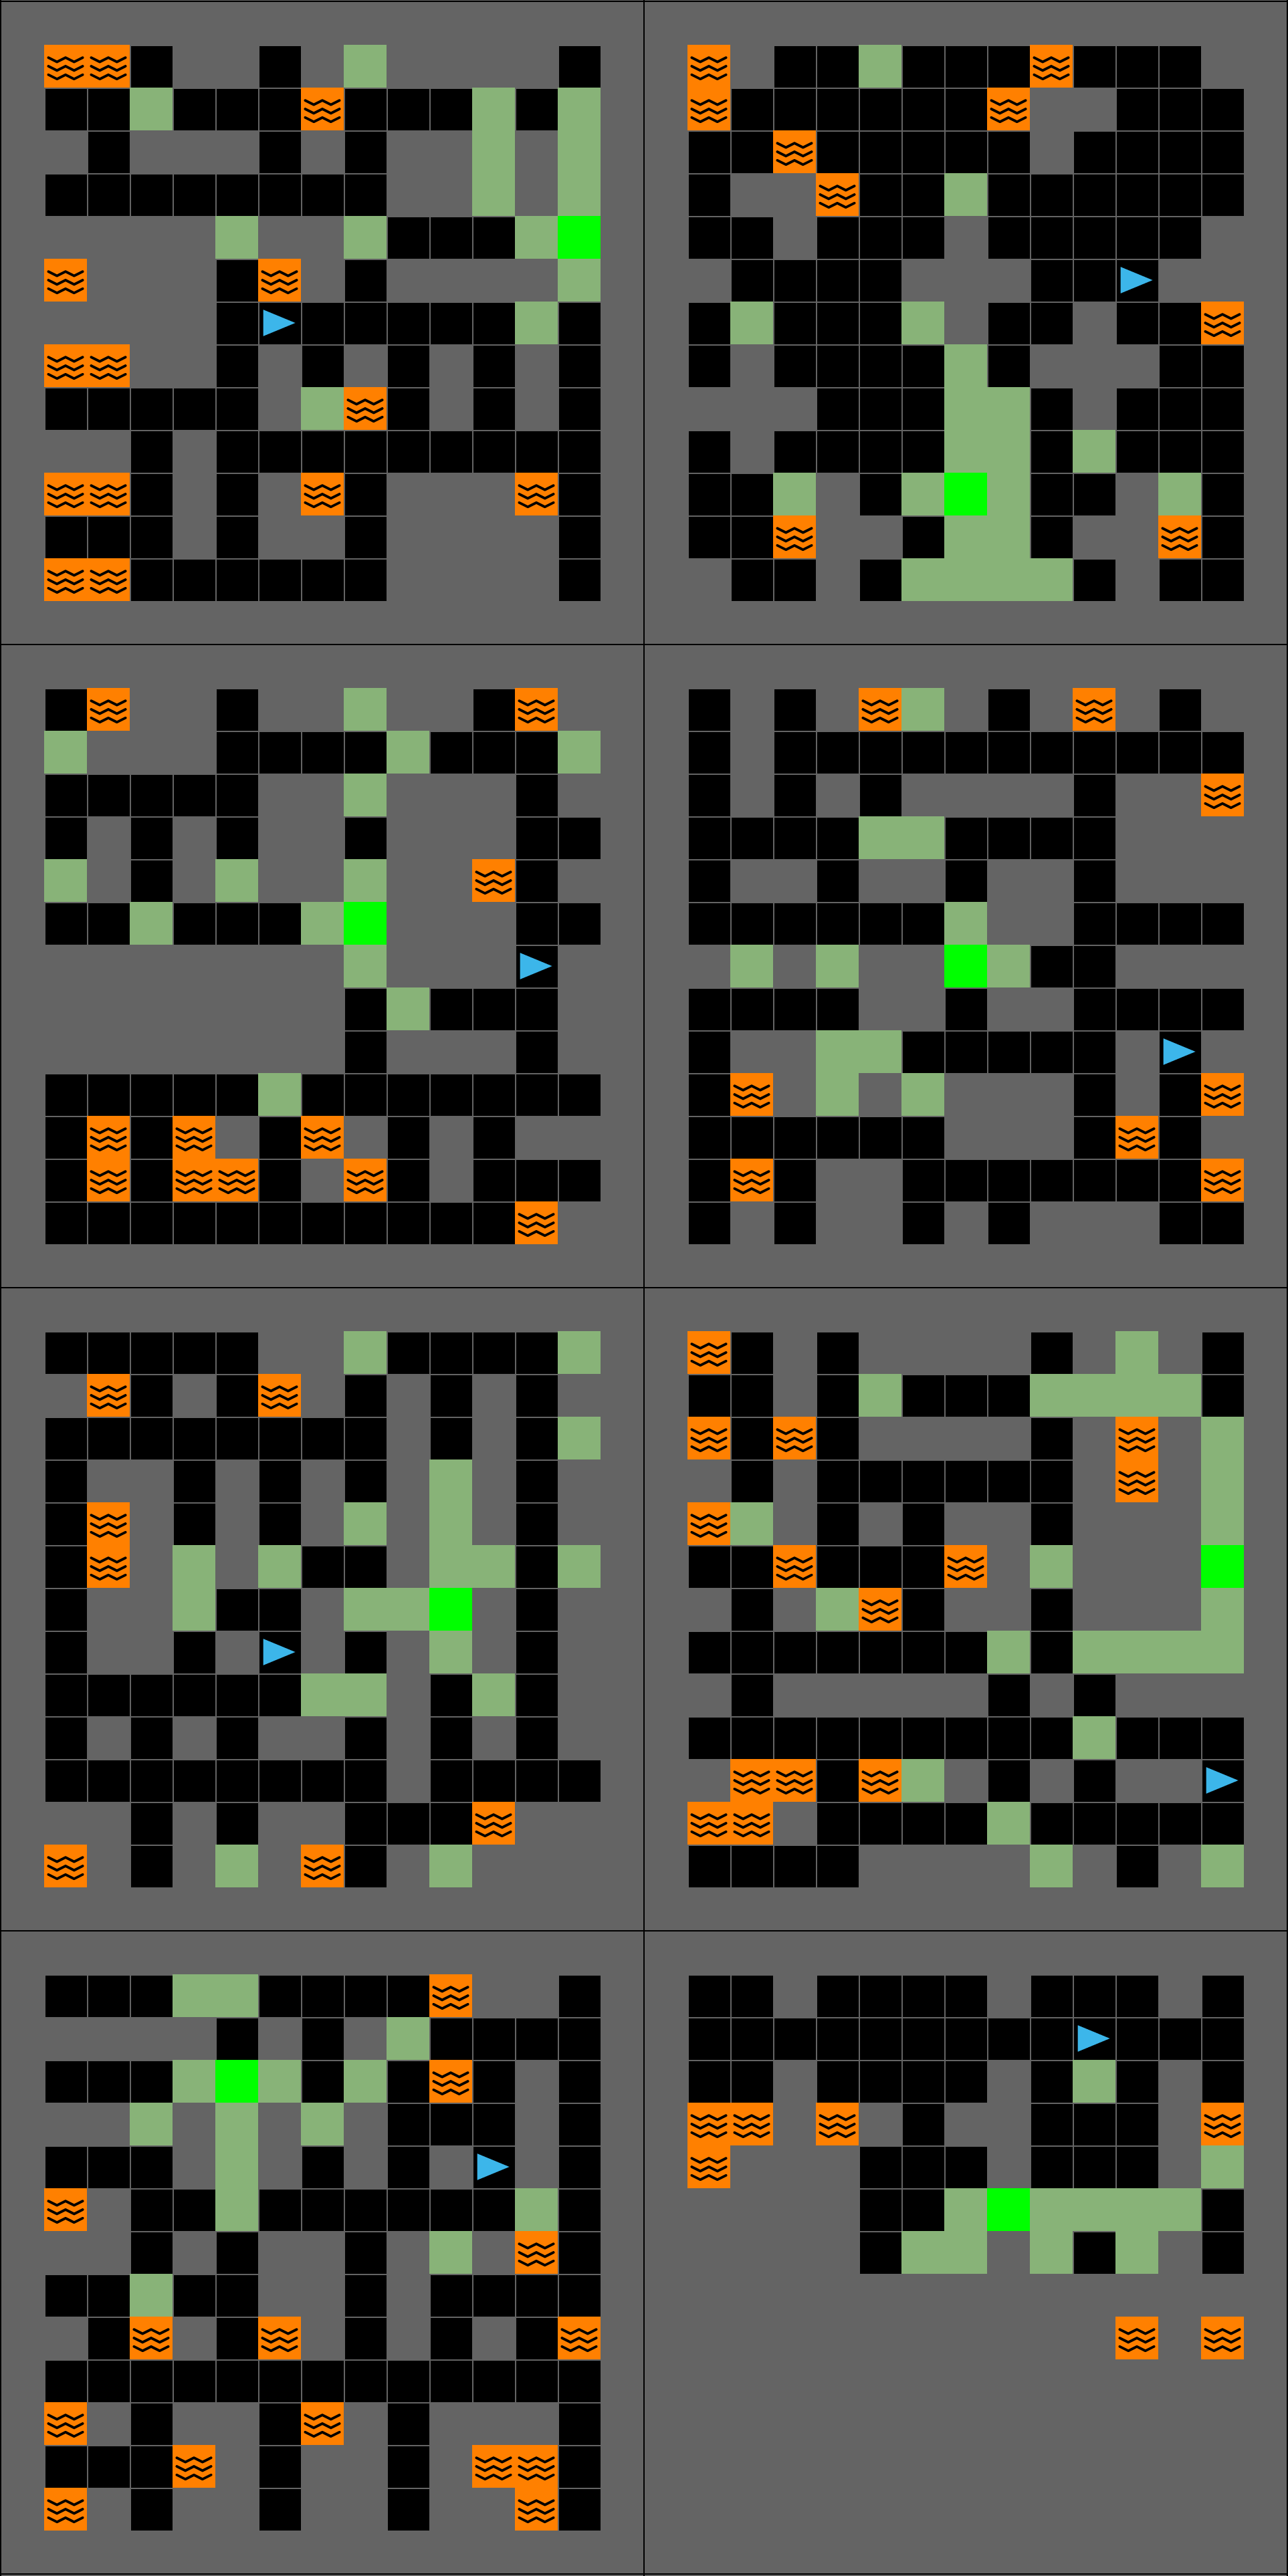
\includegraphics[height=3cm]{app_content/layouts/base_levels_crop.png}%
    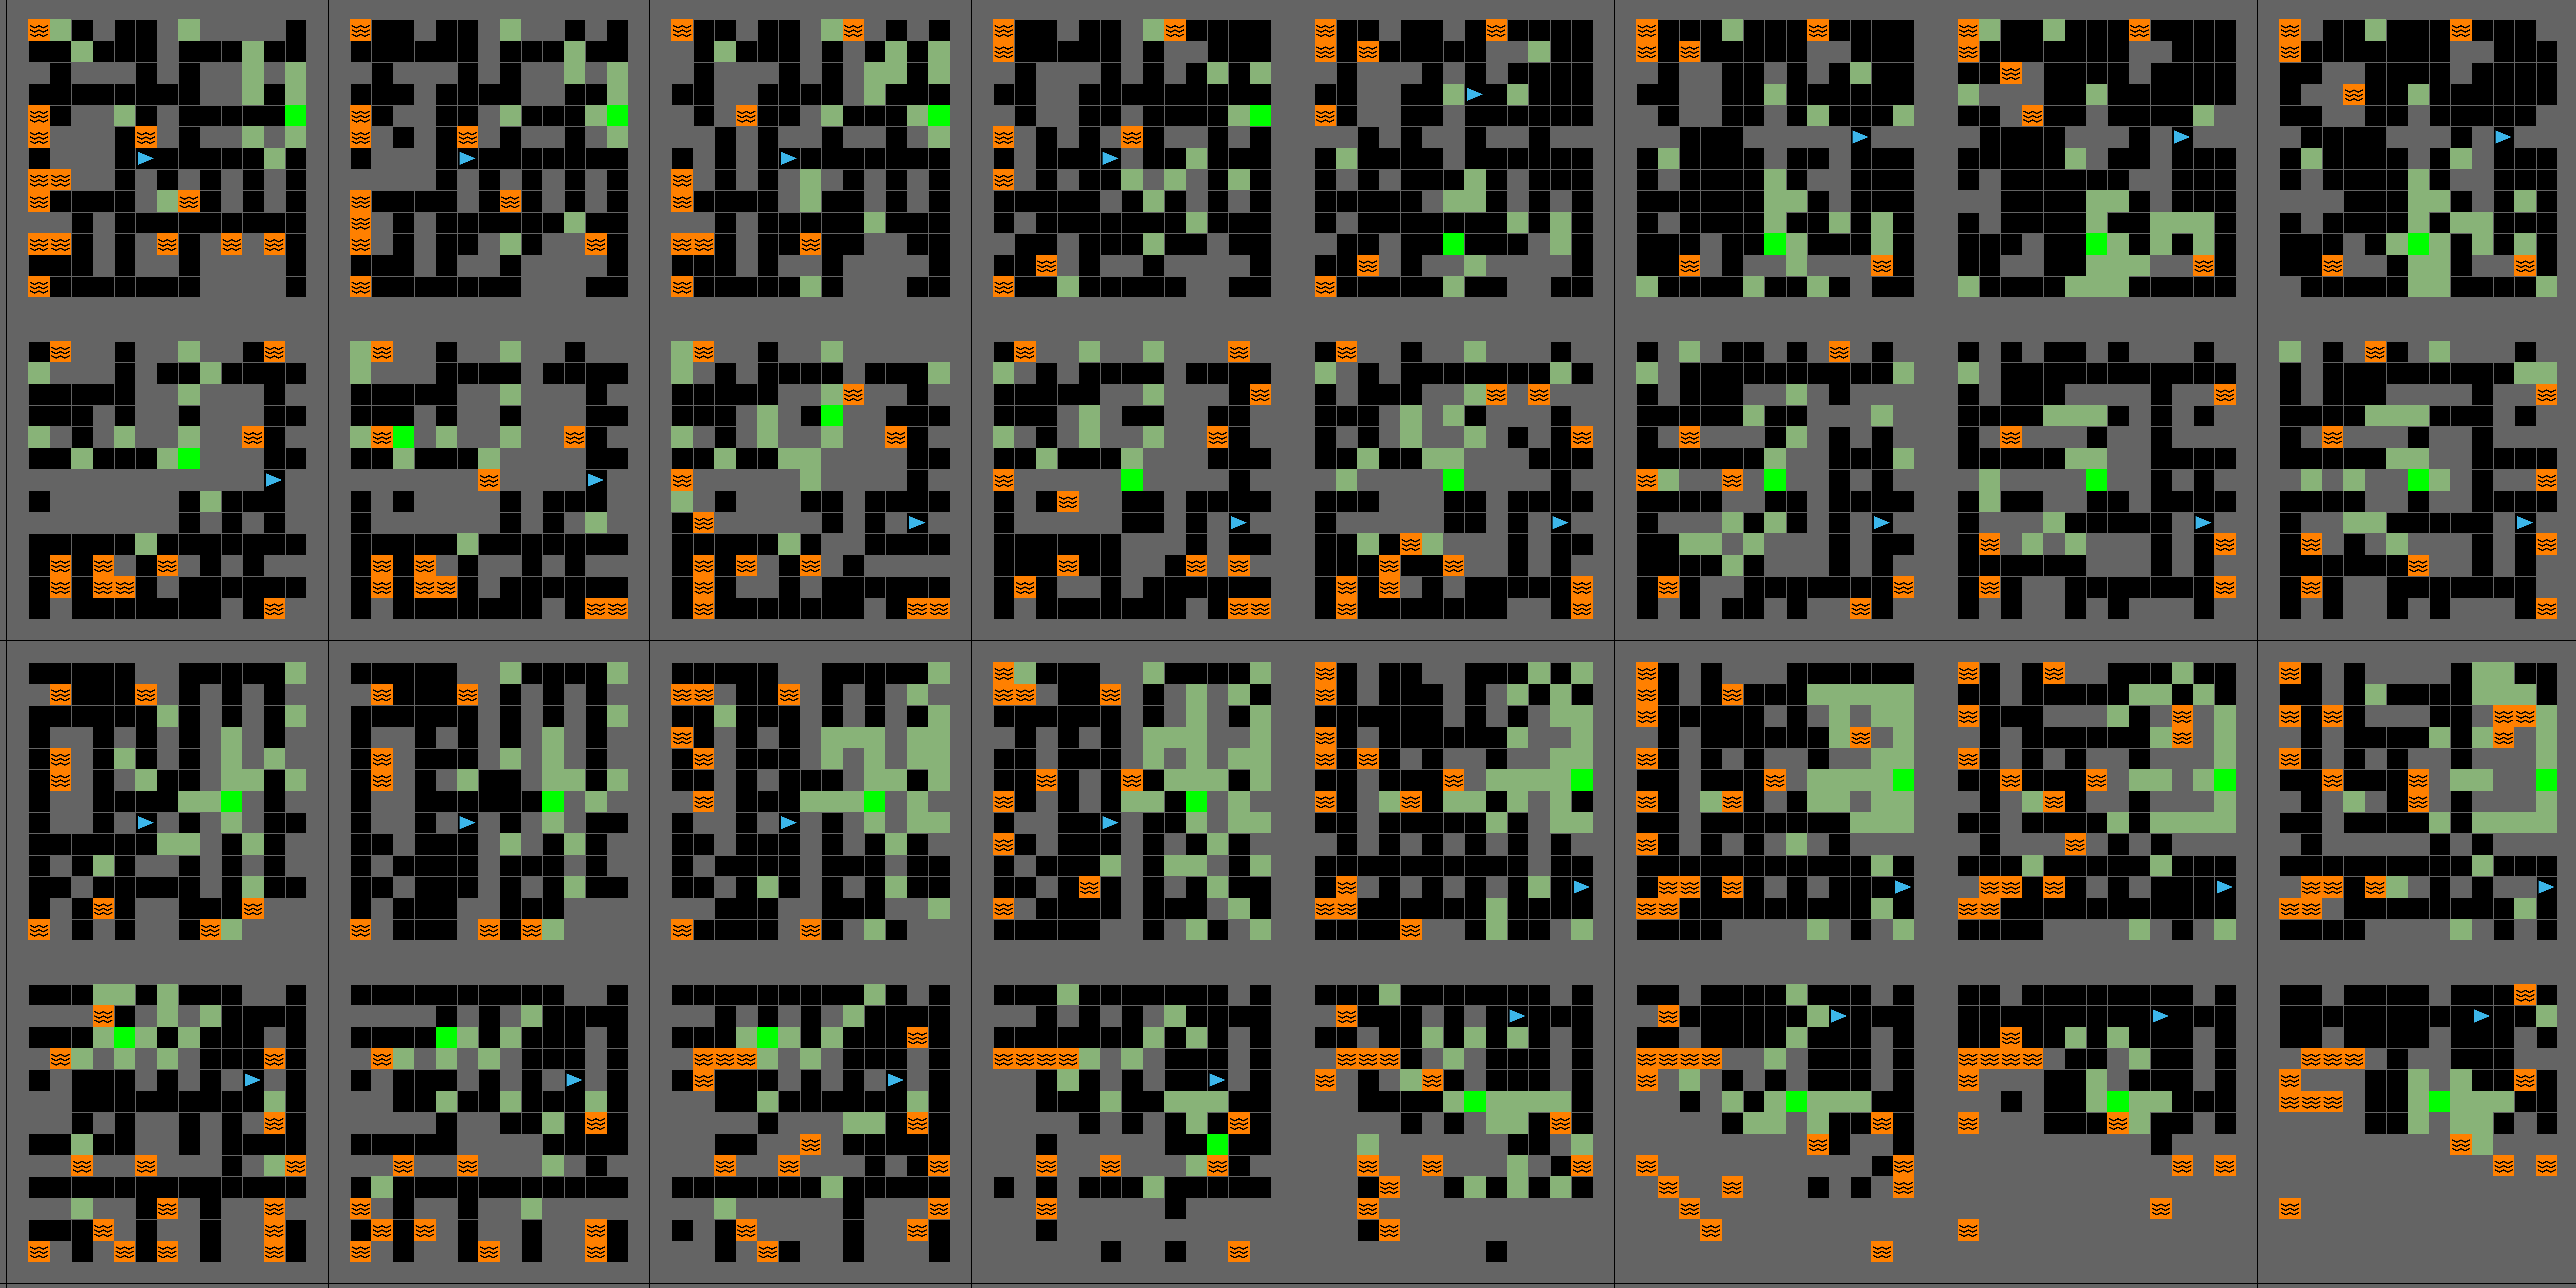
\includegraphics[height=3cm]{app_content/layouts/interp_levels_crop.png}%
  }%
}
\setlength{\twosubht}{\ht\twosubbox}

% typeset

\centering

\subcaptionbox{Parent levels sampled from $X_\text{train}$}{%
  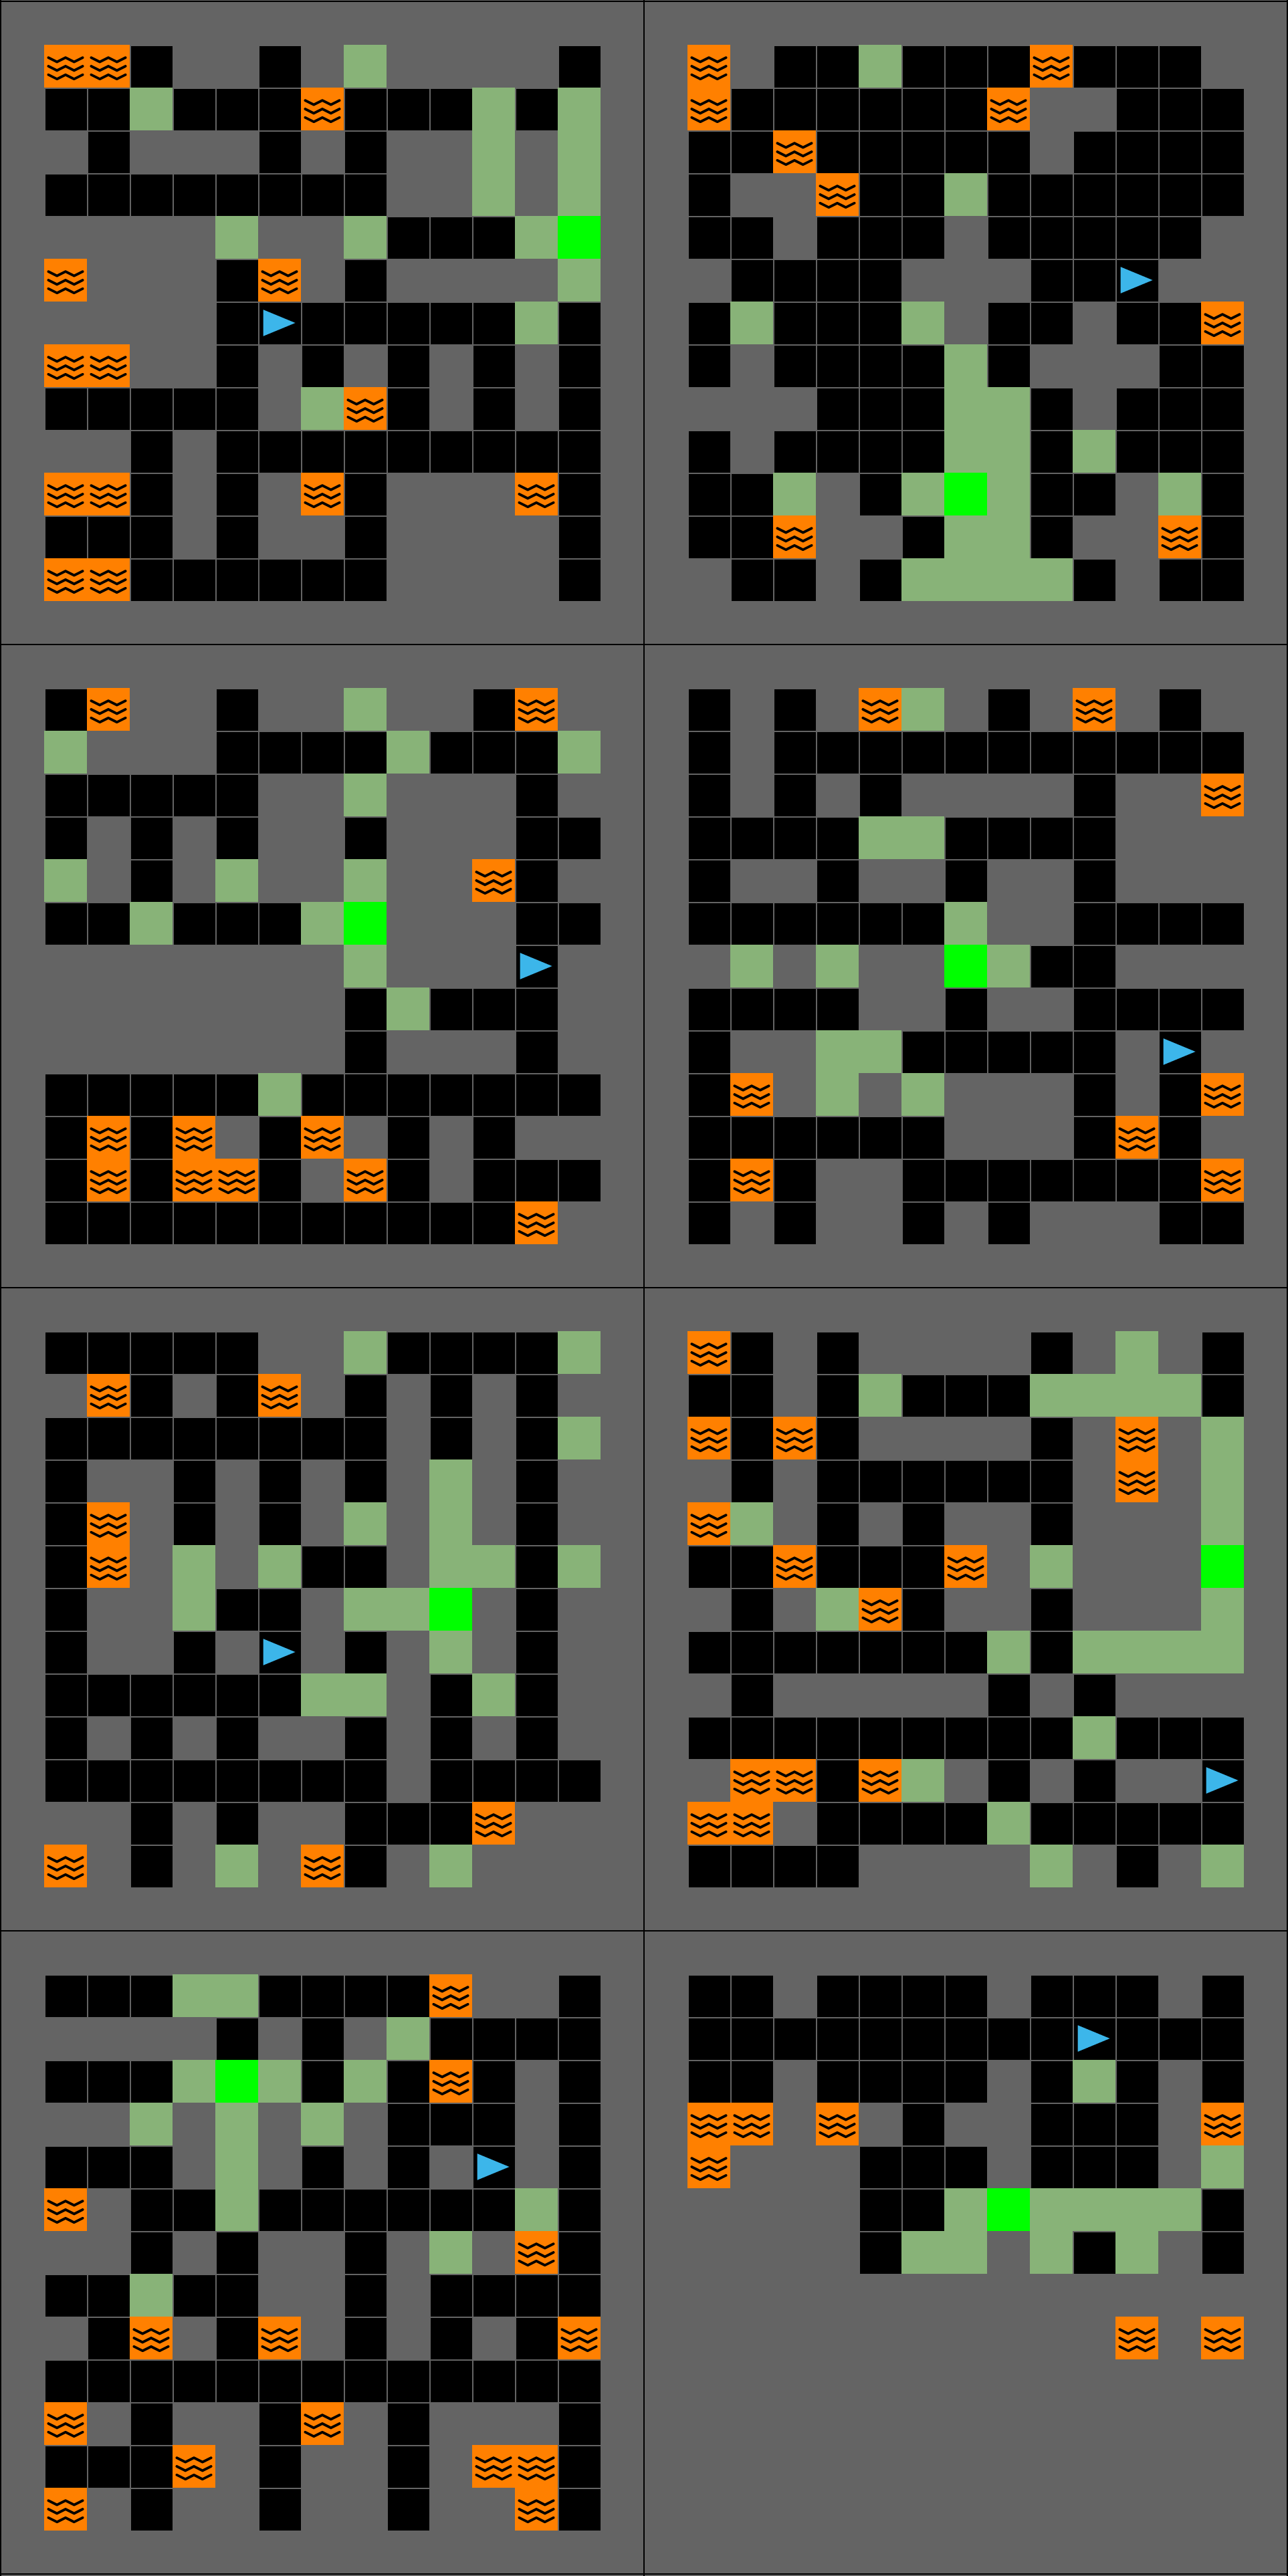
\includegraphics[height=\twosubht]{app_content/layouts/base_levels_crop.png}%
}\quad
\subcaptionbox{Levels generated by the VAE}{%
  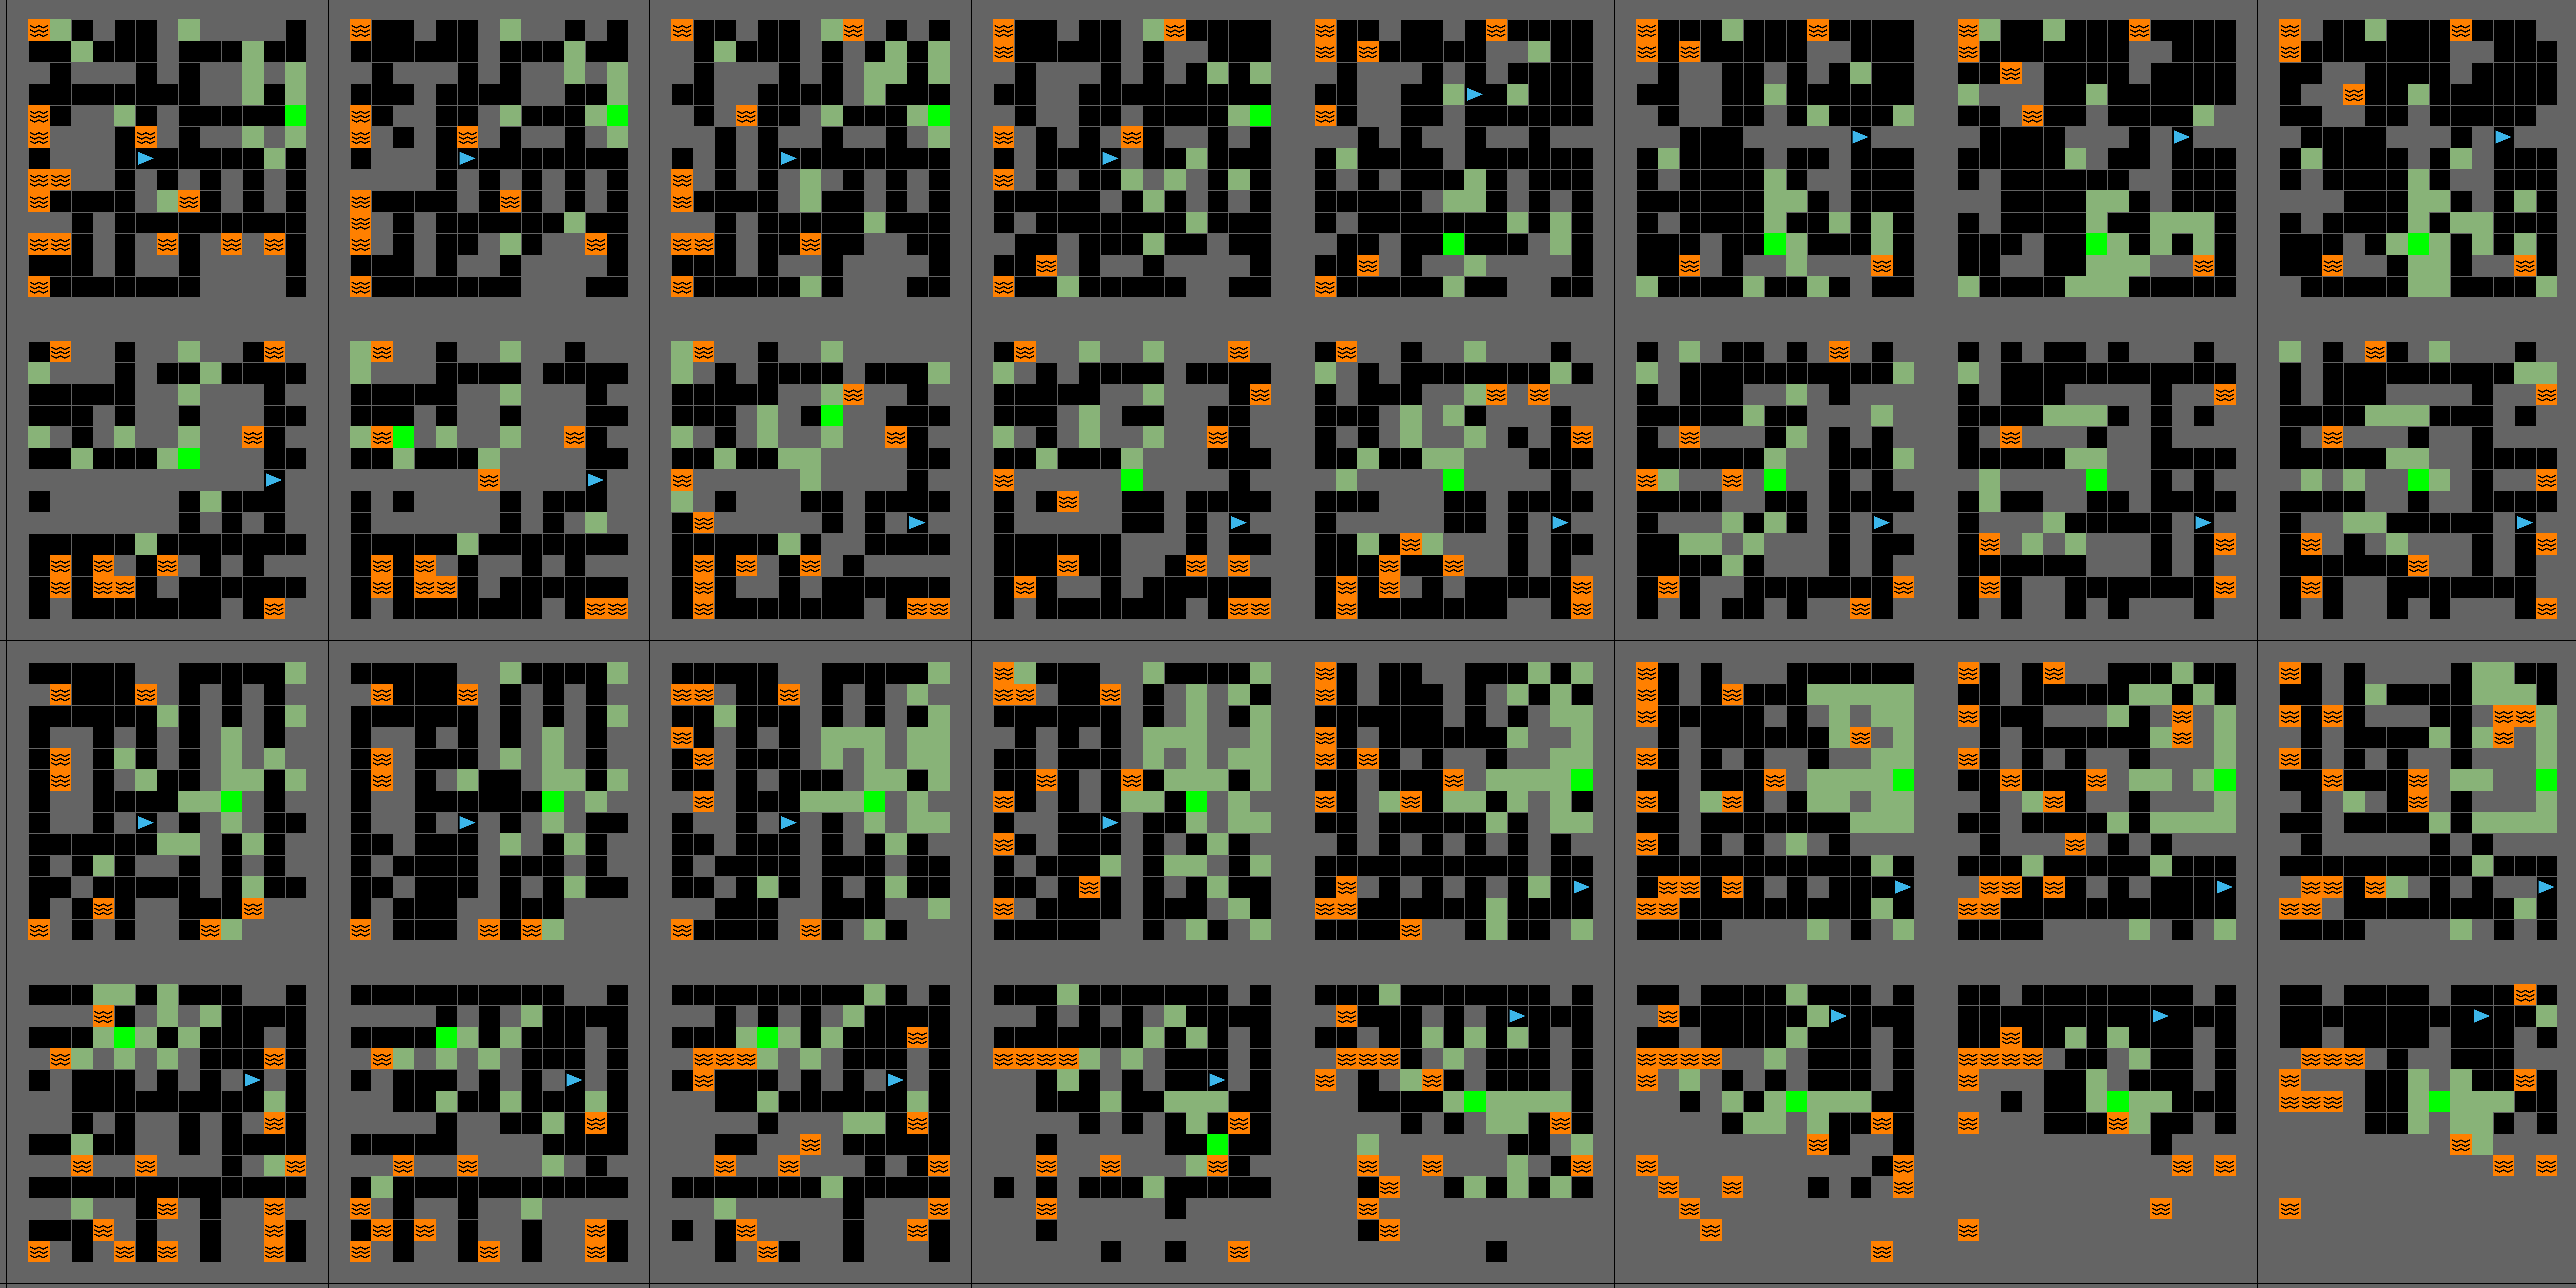
\includegraphics[height=\twosubht]{app_content/layouts/interp_levels_crop.png}%
}

\caption{Sample of levels generated by interpolating within the latent space of the VAE. On the right, each row represents an interpolation between the latent embeddings of a pair of base levels (on the left). The layouts generated are not always solvable, but, when they are solvable, they tend to retain semantics consistent with the CMDP.}\label{fig:interpolated_levels}

\end{figure}


 % $\gG_\vx$ is given as input to a Graph Convolutional Network (GCN), a generalisation of the Convolutional Neural Network \citep{CNNimagenet} to non Euclidian spaces. We select the GIN architecture \citep{GIN} for the GCN due to its higher expressivity compared to other GCN variants. We train our model by minimising \ref{eq:ELBO}, successively encoding and reconstructing $\gG_\vx$.

\begin{table}[!htb]
\caption{Hyperparameters used for Minigrid experiments. Hyperparameters shared between methods are only reported if they change from the method above.}
\label{table:hyperparams}
\begin{center}
\scalebox{0.88}{
\begin{tabular}{lcccc}
\toprule
\textbf{Parameter} & Procgen & MiniGrid\\
\midrule
\emph{PPO} & \\
$\gamma$ &0.999 & 0.995 \\
$\lambda_{\text{GAE}}$ & 0.95 & 0.95  \\
PPO rollout length & 256 & 256 \\
PPO epochs & 3 & 5 \\
PPO minibatches per epoch & 8 & 1 \\
PPO clip range & 0.2 & 0.2 \\
PPO number of workers & 64 & 32 \\
Adam learning rate & 5e-6 & 1e-4 \\
Adam $\epsilon$ & 1e-5 & 1e-5  \\
PPO max gradient norm & 0.5  & 0.5  \\
PPO value clipping & yes  & yes \\
return normalisation & yes & no \\
value loss coefficient & 0.5 & 0.5 \\

\addlinespace[10pt]
\emph{PLR} & & & \\
Scoring function & $\ell_1$-value loss  & $\ell_1$-value loss \\
Replay rate, $p$ & 1.0 & 1.0 \\
Buffer size, $K$ & 200 & 512 \\
Prioritisation, & rank & rank \\
Temperature, & 0.1  & 0.1 \\
Staleness coefficient, $\rho$ & 0.1  & 0.3 \\

\addlinespace[10pt]
\emph{RPLR} & & & \\
Scoring function, & & positive value loss \\
Replay rate, $p$ &  & 0.5 \\
Buffer size, $K$ &  & 4000 \\

\addlinespace[10pt]
\emph{ACCEL} & & \\
Edit rate, $q$ & & 1.0 \\
Replay rate, $p$ & & 0.8 \\
Buffer size, $K$ & & 4000 \\
Edit method, & & random  \\
Levels edited, & & easy \\

\addlinespace[10pt]
\emph{VAE-DRED} & & & \\
Replay rate, $p$ & & 1.0 \\
Scoring function support, & & dataset \\
Staleness support, &  & dataset \\
Secondary Scoring function, & & $\ell_1$-value loss \\
Secondary Scoring function support, & & buffer \\
Secondary Temperature, & & 1.0 \\
Mixing coefficient, $\eta$ & & linearly increased from 0 to 1 \\

\bottomrule 
\end{tabular}
}
\end{center}
\end{table}

\begin{table}[!htb]
\caption{Hyperparameters used for pre-training the VAE.}
\label{table:hyperparams_vae}
\begin{center}
\scalebox{0.88}{
\begin{tabular}{lccc}
\toprule
\textbf{Parameter} & \\
\midrule
\emph{VAE} & \\
$\beta$ & 0.0448 \\
layout head reconstruction coefficient & 0.04 \\
start and goal heads reconstruction coefficients & 0.013 \\
number of variational samples & 1 \\
Adam learning rate & 4e-4 \\
Latent space dimension & 1024 \\
number of encoder GCN layers & 4 \\
encoder GCN layer dimension & 12 \\
number of encoder MLP layers (including bottleneck layer) & 2 \\
encoder MLP layers dimension & 2048 \\
encoder bottleneck layer dimension & 256 \\
number of decoder layers & 3 \\
decoder layers dimension & 256 \\


\bottomrule 
\end{tabular}
}
\end{center}
\end{table}

\begin{figure}[!htb]
    \centering
            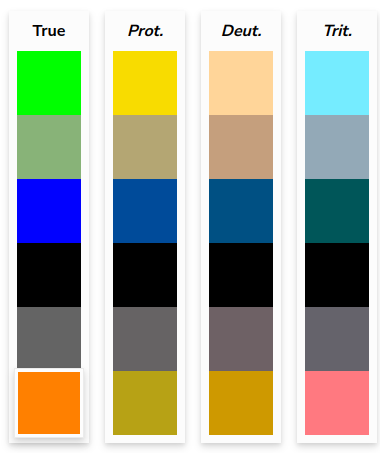
\includegraphics[width=.4\linewidth]{app_content/misc/Color_palette_color_blindness.png}
    \caption{Color palette used for rendering minigrid layouts in this paper and their equivalent for Protanopia (Prot.), Deuteranopia (Deut.) and Tritanopia (Trit.) color blindness. We refer to each row in the main text as, in order: green (goal tiles), pale green (moss tiles), blue (agent), black (empty/floor tiles), grey (wall tiles) and orange (lava tiles).
    }
    \label{fig:color_palette}
\end{figure}